\documentclass[11pt]{article}
\usepackage[T1]{fontenc}
\usepackage{lmodern}
\usepackage[margin=1.05in]{geometry}
\usepackage{amsmath,amssymb,amsthm,mathtools,booktabs,array,longtable}
\usepackage{microtype}
\usepackage{tikz}
\usetikzlibrary{arrows.meta,positioning}
\usepackage{xcolor}
\definecolor{linkblue}{RGB}{20,69,103}
\usepackage[colorlinks=true,linkcolor=linkblue,citecolor=linkblue,urlcolor=linkblue]{hyperref}
\hypersetup{pdftitle={From partial permutation information to Fourier bounds},pdfauthor={OpenAI},bookmarksnumbered=true}
\newtheorem{theorem}{Theorem}[section]
\newtheorem{lemma}[theorem]{Lemma}
\newtheorem{proposition}[theorem]{Proposition}
\newtheorem{corollary}[theorem]{Corollary}
\theoremstyle{definition}\newtheorem{definition}[theorem]{Definition}
\theoremstyle{remark}\newtheorem{remark}[theorem]{Remark}
\newcommand{\E}{\mathbb E}
\newcommand{\TV}{\mathrm{TV}}
\newcommand{\op}{\mathrm{op}}
\newcommand{\HS}{\mathrm{HS}}
\newcommand{\id}{\mathrm{id}}
\newcommand{\one}{\mathbf1}
\newcommand{\F}{\mathbb F_2}
\newcommand{\Unif}{\operatorname{Unif}}
\newcommand{\norm}[1]{\left\lVert#1\right\rVert}
\DeclareMathOperator{\tr}{tr}
\DeclareMathOperator{\Sym}{Sym}
\DeclareMathOperator{\Span}{span}
\DeclareMathOperator{\sgn}{sgn}
\DeclareMathOperator{\Irr}{Irr}
\numberwithin{equation}{section}
\title{From partial permutation information to Fourier bounds}
\author{OpenAI}
\date{September 26, 2026}
\begin{document}
\maketitle
\begin{abstract}
We show how information about partial permutations controls full permutation laws. Let $n$ tend to infinity through multiples of eight. If the images of a uniformly chosen $7n/8$ labels approach the uniform injection law in average total variation, and the sign mean tends to zero, then the product of two independent permutations with the given law converges to uniform on $S_n$.
\end{abstract}
\section{What partial observations can determine}
\label{l:introduction}

A permutation can look uniform on many labels while retaining information about the whole deck. Parity gives the simplest example: the uniform law on the alternating group has uniform images on any set of at most $n-2$ labels. Thus partial observations require an additional argument before they can establish convergence on $S_n$. This paper develops that argument. Its input is quantitative information about partial permutations; its output is a bound on every nontrivial Fourier matrix, with the sign representation treated separately.

Let $X$ be a set of $n$ labels and $G=\Sym(X)$. We regard $g\in G$ as the map from initial labels to final positions. For $M\subseteq X$, let $H_M=\Sym(M)$ fix $X\setminus M$ pointwise. Two permutations have the same images on $X\setminus M$ precisely when they lie in the same left coset $gH_M$. Consequently an upper bound on the distribution of those images is exactly an upper bound on the masses of these cosets. The elements of $gH_M$ are obtained by multiplication on the right; this convention matters when image observations are compared with inverse-image observations.

For a nonnegative measure $f$ on $G$ and an irreducible unitary representation $\rho:G\to U(V_\rho)$, write
\[
 \widehat f(\rho)=\sum_{g\in G}f(g)\rho(g),\qquad D_\rho=\dim V_\rho.
\]
Our Hilbert--Schmidt norm is unnormalized: $\|A\|_{\HS}^2=\tr(A^*A)$. Let $D_\lambda$ denote the degree of the irreducible of $S_m$ indexed by a partition $\lambda\vdash m$, and set
\[
 C_u=\sup_{m\ge1}\sum_{\lambda\vdash m}D_\lambda^{-u}\quad(u>0).
\]
These constants are finite, and the sums with the row and column partitions removed tend to zero. A short proof is given in Lemma~\ref{l:degree-basic}; Section~\ref{l:degrees} retains the distinct counting proofs that give more detailed information.

\begin{theorem}[Complementary cosets control Fourier matrices]
\label{l:main}
Partition $X$ into $b$ nonempty sets $M_1,\ldots,M_b$. Put $H_i=H_{M_i}$. Suppose $f$ is a nonnegative measure on $G$ of mass at most one and, for every $g\in G$ and $i$,
\begin{equation}\label{l:main-cap}
 f(gH_i)\le \frac{B}{[G:H_i]}.
\end{equation}
For every $u>0$ and every irreducible $\rho$ of degree $D$,
\begin{equation}\label{l:main-hs}
 \|\widehat f(\rho)\|_{\HS}^2
 \le bBC_uD^{-1+(u+2)/b}.
\end{equation}
There is also an independent orbit-span proof of the bound
\begin{equation}\label{l:main-orbit}
 \|\widehat f(\rho)\|_{\op}^2
 \le bBC_uD^{-1+(u+2)/b}.
\end{equation}
No restriction is imposed on block sizes or on the multiplicities in $\rho|_{H_1\times\cdots\times H_b}$.
\end{theorem}

The Hilbert--Schmidt conclusion implies the operator-norm conclusion, but the two proofs use different information. The orbit proof follows one vector and controls the dimension of its orbit under a small subgroup type. The isotypic proof instead bounds the entire Fourier matrix by cosetwise Plancherel. We give the orbit proof first because it isolates the multiplicity issue in a concrete linear map, and then prove the stronger norm conclusion independently.

The principal consequence is a transfer from observations of $7n/8$ labels to the product of just two independent permutations. Suppose $8$ divides $n$, the average total-variation error of these observations tends to zero, and the sign mean is $o(1)$. One can choose eight complementary blocks whose errors sum to $o(1)$, then retain a common subprobability of mass $1-o(1)$ with coset cap one. With $b=8$ and $u=1$, Theorem~\ref{l:main} gives squared Hilbert--Schmidt norm at most $8C_1D^{-5/8}$. Two convolutions have nonsign Plancherel contribution at most $(8C_1)^2\sum D^{-1/4}$, which tends to zero. The discarded mass and sign coefficient also vanish. Corollary~\ref{l:isotypic-completion} gives the precise conclusion. The orbit proof alone gives four convolutions, as recorded in Corollary~\ref{l:orbit-completion}. The distinction is the dimension factor saved by controlling the whole matrix, not a change in the observed marginals.

\subsection{The first proof and its extensions}

Restriction to $H_1\times\cdots\times H_b$ decomposes an irreducible space into tensor-product types, each tensored with its multiplicity space. The product of the factor degrees is at most $D$. Hence some factor has degree at most $D^{1/b}$. Assign the whole type to one such factor. This produces an orthogonal decomposition of any test vector into $b$ pieces. The orbit of one piece under its assigned subgroup has dimension at most the sum of the squares of the small factor degrees. Multiplicity causes no extra factor: on all copies of one type the group acts by the same matrix tensored with identity. The bound $C_u$ now controls that sum. Averaging the projections onto translates of the orbit span, Schur's lemma turns its dimension into a factor $1/D$. This proves \eqref{l:main-orbit}.

The next proof retains more of the Fourier matrix. The central idempotent of a subgroup type projects onto all its copies. Cosetwise convolution bounds the squared Hilbert--Schmidt norm of the projected transform, summed over every ambient irreducible. The small subgroup types cover the original representation; taking a trace against a positive operator completes \eqref{l:main-hs}. This also explains why one must count types once rather than count their multiplicities.

The complete fixed-coset route is proved in Sections~\ref{l:foundations}--\ref{l:core-section}. Sections~\ref{l:comparisons-section} and~\ref{l:random-partition-section} compare alternative coefficient arguments and retained measures for the same marginal information. Section~\ref{l:degrees} develops the shape-sensitive degree estimates needed later, and Section~\ref{l:characters-section} constructs one-dimensional characters in subgroups of controlled index. Supplementary tableau and hook proofs are grouped in Appendix~\ref{l:degree-supplement}. Appendix~\ref{l:transfer-supplement} retains the projection-averaging and longest-line peeling methods, together with explicit parameter substitutions. These independent routes remain available without interrupting the main transfers.

The remaining results distinguish three kinds of additional information. First, image and inverse-image caps control opposite sides of a Fourier matrix. Section~\ref{l:two-sided-section} places those sides together in a product of two laws. Section~\ref{l:equivariant-section} instead works with transition kernels: the sign contribution is then an operator on a multiplicity space, not merely the scalar sign mean of a group law.

Second, the quantifiers on an information bound determine which changes of law it permits. Section~\ref{l:domains-section} constructs retained laws by selecting good omitted sets separately for each permutation, under the same averaged marginal hypothesis as the fixed-partition route. Section~\ref{l:tilts-section} assumes an entropy comparison for every law on one common event; it can therefore condition on a rare representation-coefficient event. Section~\ref{l:palettes} obtains analogous rare-event control from a pointwise bound on accumulated reveal errors. In contrast, the single-law entropy bounds of Section~\ref{l:replica-section} give a growing coset cap by clipping. They control only sufficiently large dimensions; Section~\ref{l:forests} supplies a precise hybrid conclusion when a separate law handles the remaining diagrams by long-row decay and exact vanishing on diagrams with more than $n/2$ rows.

Finally, Section~\ref{l:sec:tabloid} uses a conditional product structure: after fixing an environment, the two half-permutations are independent. A signed tabloid basis turns their image caps into matrix bounds, while a preceding law's inverse-image caps average positive operators. Appendix~\ref{l:tabloid-supplement} gives an independent arm--leg construction of the signed representation used there. These different hypotheses are kept explicit; no mixing conclusion is inferred by substituting one kind of partial information for another.

\subsection{Relation to earlier methods}

Fourier analysis of random walks on finite groups converts distributional convergence into estimates of matrix transforms. Diaconis and Shahshahani's analysis of random transpositions is a fundamental example \cite{diaconis-shahshahani}; the Plancherel and total-variation steps used here belong to that framework. We keep matrix norms throughout because the laws considered here need not be central and their transforms need not be normal.

The representation-theoretic ingredients are classical. Specht modules, Young branching, induced representations from Young subgroups, and the Littlewood--Richardson rule supply the restriction and signed-tabloid constructions; see James \cite{James1978} and Sagan \cite{sagan}. The hook formula of Frame, Robinson, and Thrall \cite{frame-robinson-thrall} and elementary standard-tableau constructions supply degree lower bounds. The reciprocal-degree limits are part of the symmetric-group Witten-zeta theory; see Liebeck and Shalev \cite[Proposition~2.5 and Theorem~2.6]{liebeck-shalev2004}. We give elementary proofs suited to the different transfer arguments and retain their more detailed tableau bounds. The orbit-span and coset estimates are proved explicitly. Relative entropy enters through its chain rule and its variational behavior under conditioning; the rare-event arguments specify the changed law explicitly.

One motivation is the Thorp shuffle, introduced in \cite{Thorp1973}.
Entropy methods yielded an $O((\log n)^4)$ mixing bound for even decks
and an $O((\log n)^3)$ bound for power-of-two decks
\cite{Morris2009,Morris2013}. These bounds count elementary
cut-and-interleave shuffles; on $n=2^d$ cards, a complete coordinate
sweep consists of $d$ such steps. The entropy arguments reveal and
compare card trajectories, providing a methodological antecedent to
the partial-information hypotheses considered here.

More directly, Czumaj and V\"ocking studied the joint randomization
of a fixed fraction of labeled cards under the Thorp shuffle
\cite{CzumajVocking2014}. Czumaj subsequently obtained full-permutation
sampling by recursively applying partial-permutation randomizers on
successively smaller sets \cite{Czumaj2015}. The present transfer has
a different form: complementary quotient estimates for a single law
control its noncentral Fourier matrices and, with separate sign
control, imply mixing after a fixed number of independent compositions
of that same law. No shuffle construction or physical-time bound is
assumed in the abstract proofs.

Three companion papers construct inputs for the later transfers.
The coordinate-frame paper proves the all-tilt entropy estimate in
Lemma~12.13 and establishes the quotient and retained sign-multiplicity
estimates within the proof of Theorem~14.2 \cite{companion-frames}.
The conditional-information paper supplies the fixed-list estimate in
Proposition~3.3; the palette estimate and common-event construction in
Proposition~13.2 and equations~(13.2)--(13.3); the random-domain
estimate in Theorem~12.2; the weak-entropy and sparse-Fourier inputs in
Propositions~15.1 and~15.4; and the entropy assertion~(16.1) of
Theorem~16.1 \cite{companion-information}.
The conditional-permutation paper constructs the two-half environment
and its independent internal permutations in the proof of Theorem~7.1
and Lemma~7.2 \cite{companion-kernels}.
These estimates are established before the cited papers apply the
transfer results here. Their full-deck mixing conclusions are
applications, not hypotheses of the present proofs; their discarded-mass,
parity, and physical-time checks remain part of those applications.

\section{Degree sums, common trimming, and normalization}
\label{l:foundations}

We first supply the three ingredients needed to complete a transfer: a uniform count of small representation degrees, one measure satisfying all coset bounds at once, and the precise Fourier conversion to total variation. For a finite set, $U$ denotes uniform probability. For a subgroup $H\le G$, the pushforward of $\mu$ to $G/H$ is denoted by $\mu_H$, so $\mu_H(gH)=\mu(gH)$. Our convention is $\|\mu-\nu\|_{\TV}=\frac12\sum_x|\mu(x)-\nu(x)|$ for probabilities.

\begin{lemma}[A short reciprocal-degree proof]\label{l:degree-basic}
For every $u>0$, $C_u<\infty$ and
\[
 Z_u(n):=\sum_{\lambda\vdash n,\ \lambda\notin\{(n),(1^n)\}}D_\lambda^{-u}\longrightarrow0.
\]
The excluded partitions form a set, so the unique partition of one is removed only once.
\end{lemma}
\begin{proof}
We use the classical tableau dimension and hook formulas: $D_\lambda$ is the number of fillings of the diagram of $\lambda$ by $1,\ldots,n$ increasing along each row and column, and
\[D_\lambda=\frac{n!}{\prod_{x\in\lambda}h(x)},\]
where $h(x)$ counts the box $x$ and the boxes strictly right of it or strictly below it \cite{frame-robinson-thrall,James1978}. Write $p(k)$ for the number of partitions of $k$, with $p(0)=1$. Euler's product at $x=e^{-1/\sqrt{k}}$ gives, for $k\ge1$,
\[
 \log p(k)\le\sqrt{k}+\sum_{j\ge1}\frac1{j(e^{j/\sqrt{k}}-1)}
 \le\sqrt{k}\left(1+\sum_{j\ge1}j^{-2}\right)\le3\sqrt{k}.
\]
If a Young diagram has a top row of length $a$ and $j\le a$ lower boxes, its number of standard tableaux is at least $\binom aj$. Put the first $j$ labels in the first $j$ top-row positions, choose the $j$ lower labels from the remaining $a$ labels, and fill the lower diagram in one fixed standard relative order. Its width is at most $j$, so every top-row predecessor is smaller. Fill the rest of the row increasingly. A tableau of any Young subdiagram extends to the full diagram by adding larger labels in an order respecting row and column predecessors.

Orient a longest row or column as the first row and let its length be $n-j$. When $1\le j\le n/3$, at most $2p(j)$ diagrams have this value and
\[
 D_\lambda\ge\binom{n-j}{j}\ge2^j.
\]
For each fixed $j>0$ the binomial coefficient diverges, and $2p(j)2^{-uj}$ is summable. Dominated convergence handles this range.

In the remaining range put $a=\max(\lambda_1,\lambda'_1)<2n/3$. If $a\ge n/10$, retain the first row and a lower Young order ideal of $\lfloor a/2\rfloor$ boxes; there are enough lower boxes. Extension and the preceding construction give $D_\lambda\ge2^a/(a+1)$, exponential in $n$. If $a<n/10$, every hook has length at most $2a$, and the hook formula gives $D_\lambda\ge n!/(2a)^n\ge(5/e)^n$. Both bounds beat $p(n)\le e^{3\sqrt n}$. Thus $Z_u(n)\to0$. Adding the row and column shows that the full sum tends to two; finitely many smaller values are finite.
\end{proof}

\begin{lemma}[Selecting one partition]\label{l:partition-selection}
If $n$ is divisible by $b$ and a law $\mu$ on $S_n$ satisfies
\[
 \E_{|M|=n/b}\|\mu_{H_M}-U_{G/H_M}\|_{\TV}\le\delta,
\]
there is a partition into $b$ equal blocks for which the sum of the complementary coset errors is at most $b\delta$.
\end{lemma}
\begin{proof}
Every block of a uniformly chosen ordered equal partition is itself a uniform $n/b$-subset. The expected sum of the errors is at most $b\delta$, so one partition has sum no larger than that expectation.
\end{proof}

\begin{lemma}[Two common trimming operations]\label{l:trim}
Let $H_1,\ldots,H_b$ be subgroups of a finite group $G$, let $\mu$ be a probability, and put $\delta_i=\|\mu_{H_i}-U_{G/H_i}\|_{\TV}$ and $\delta=\sum_i\delta_i$.
There is a subprobability $f\le\mu$ with
\[
 f(G)\ge1-\delta,\qquad f(gH_i)\le[G:H_i]^{-1}\quad(g\in G,i\le b).
\]
For any $c>1$, deleting the union of all cosets with original density greater than $c$ loses mass at most $c\delta/(c-1)$. If that loss is $\eta<1$, the conditional law $\nu$ has
\[
 \|\nu-\mu\|_{\TV}=\eta,\qquad \nu(gH_i)\le\frac{c}{1-\eta}[G:H_i]^{-1}.
\]
In particular $c=2$ loses at most $2\delta$.
\end{lemma}
\begin{proof}
Process the subgroup coset systems successively. Within each coset whose current mass exceeds its uniform mass, multiply all current point masses by the ratio of the cap to the current mass. The loss at stage $i$ is at most the original positive excess on the $i$th quotient, namely $\delta_i$, because all current masses are below $\mu$. Later decreases preserve earlier caps.

There is also a simultaneous construction with the same guarantee. For each $i$, trim $\mu$ separately to a measure $f_i$, and set $f(g)=\min_i f_i(g)$. Then $f\le f_i$ ensures every cap, while $\mu-f\le\sum_i(\mu-f_i)$ bounds the loss by $\delta$. Thus these two constructions need not produce the same measure, but prove exactly the same assertion.

If a coset $Q$ has $\mu(Q)>cU(Q)$, then $\mu(Q)\le c(\mu(Q)-U(Q))/(c-1)$. Summing over its heavy cosets and then over subgroup systems bounds the removed mass. A surviving coset has original mass at most $cU(Q)$; division by $1-\eta$ gives the displayed cap. Conditioning deletes mass $\eta$ and adds that same mass on the retained set, proving the variation equality.
\end{proof}

\begin{lemma}[Plancherel with a mass deficit]\label{l:plancherel}
For every complex mass function $a$ on a finite group $G$,
\[
 |G|\sum_g|a(g)|^2=\sum_{\rho\in\Irr(G)}D_\rho\|\widehat a(\rho)\|_{\HS}^2.
\]
If $f\ge0$ has mass $z\le1$, then
\begin{align}
 |G|\sum_g|f(g)-zU(g)|^2&=\sum_{\rho\ne\one}D_\rho\|\widehat f(\rho)\|_{\HS}^2,\label{l:centered-plancherel}\\
 \left(\sum_g|f(g)-U(g)|\right)^2&\le(1-z)^2+\sum_{\rho\ne\one}D_\rho\|\widehat f(\rho)\|_{\HS}^2.\label{l:deficit-plancherel}
\end{align}
If $f\le\mu$ for a probability $\mu$, its normalization, when $z>0$, is at variation distance at most $1-z$ from $\mu$.
\end{lemma}
\begin{proof}
Expand the squared Hilbert--Schmidt norms. The regular-character identity
\[\sum_\rho D_\rho\chi_\rho(h^{-1}g)=|G|\one_{g=h}\]
proves Plancherel. Apply it to $f-zU$, whose trivial coefficient is zero, and to $f-U$, whose trivial coefficient is $z-1$. Cauchy--Schwarz gives \eqref{l:deficit-plancherel}. Finally, $\sum|f/z-f|=1-z=\sum|\mu-f|$, so the triangle inequality proves the normalization claim.
\end{proof}

With convolution $(f*k)(g)=\sum_xf(x)k(x^{-1}g)$, transforms multiply in the displayed order. If $f\le\mu$, positivity implies $f^{*r}\le\mu^{*r}$ and the missing mass is $1-z^r\le r(1-z)$. If $\mu$ has sign mean $s$, then $|\widehat f(\sgn)|\le |s|+1-z$. For nearby probabilities, the corresponding sign perturbation is at most twice their total-variation distance.

\begin{proposition}[Fourier amplification]\label{l:amplification}
Let $\mu_n$ be probabilities on $S_n$ with $\widehat\mu_n(\sgn)=o(1)$. Suppose either $f_n$ is a nonnegative subprobability with $f_n\le\mu_n$ and mass tending to one, or $f_n$ is a probability with $\|f_n-\mu_n\|_{\TV}=o(1)$. If, uniformly for every irreducible of degree $D>1$,
\[
 \|\widehat f_n\|_{\op}\le A D^{-\beta},
\]
where $A,\beta>0$ are fixed, then $\|\mu_n^{*r}-U\|_{\TV}\to0$ for every fixed integer $r$ with $2-2r\beta<0$.
If instead $\|\widehat f_n\|_{\HS}^2\le A D^{-\gamma}$, the sufficient condition is $1-r\gamma<0$.
\end{proposition}
\begin{proof}
The sign term tends to zero by the preceding mass bounds. In the operator case,
\[
 D\|\widehat f_n^{\,r}\|_{\HS}^2\le D^2\|\widehat f_n\|_{\op}^{2r}\le A^{2r}D^{2-2r\beta}.
\]
In the Hilbert--Schmidt case submultiplicativity gives $D\|\widehat f_n^{\,r}\|_{\HS}^2\le A^rD^{1-r\gamma}$. The sums tend to zero by Lemma~\ref{l:degree-basic}. The trivial coefficient tends to one. Lemma~\ref{l:plancherel} gives convergence for $f_n^{*r}$; the missing mass or a telescoping replacement of the $r$ probability factors gives convergence for $\mu_n^{*r}$. No normality or diagonalization is used.
\end{proof}

\section{The complete transfer from disjoint coset systems}
\label{l:core-section}

The coset bounds are now available on one common measure. We first turn them into an operator estimate by following the orbit of one vector. For eight complementary coset systems, this gives convergence after four convolutions. Central projections then retain the whole Fourier matrix and reduce that count to two. Both arguments keep every restriction multiplicity; they differ in what they average.

\begin{lemma}[The orbit of a single vector]\label{l:single-orbit}
Let $H$ act unitarily on $V$, and suppose a vector $v$ has components only in $H$-types belonging to a set $\Lambda\subseteq\Irr(H)$. Then
\[
 \dim\Span\{\rho(h)v:h\in H\}\le\sum_{\tau\in\Lambda}(\dim\tau)^2.
\]
All copies of a type are included in this estimate.
\end{lemma}
\begin{proof}
Regroup the entire $\tau$-isotypic space as $V_\tau\otimes\mathcal A_\tau$, where $H$ acts as $\tau\otimes I$. If $v_\tau$ is the component of $v$ there, its orbit lies in the image of
\[
 \operatorname{End}(V_\tau)\longrightarrow V_\tau\otimes\mathcal A_\tau,
 \qquad Q\longmapsto(Q\otimes I)v_\tau.
\]
The image has dimension at most $(\dim\tau)^2$, independently of $\dim\mathcal A_\tau$. Equivalently, writing $v_\tau=\sum_{j=1}^{\dim\tau}e_j\otimes a_j$, the orbit lies in $V_\tau\otimes\Span(a_j)$. Sum over inequivalent types.
\end{proof}

Write $a=\dim\tau$, $W_\tau=\Span\{\rho(h)v_\tau:h\in H\}$, and $T(Q)=(Q\otimes I)v_\tau$. The key point is the map in Figure~\ref{l:orbit-figure}: multiplicity enlarges the ambient space, but not the matrix space that moves a fixed vector.

\begin{figure}[ht]
\centering
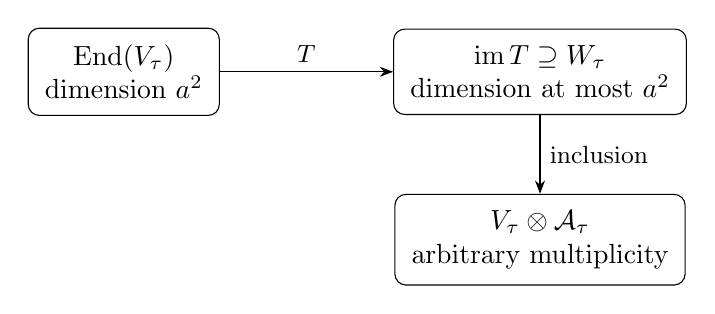
\begin{tikzpicture}[node distance=15mm,>=Stealth,
 box/.style={draw,rounded corners,align=center,inner sep=6pt}]
 \node[box] (mat) {$\operatorname{End}(V_\tau)$\\dimension $a^2$};
 \node[box,right=22mm of mat] (orbit) {$\operatorname{im}T\supseteq W_\tau$\\dimension at most $a^2$};
 \node[box,below=10mm of orbit] (ambient) {$V_\tau\otimes\mathcal A_\tau$\\arbitrary multiplicity};
 \draw[->] (mat)--node[above,font=\small] {$T$} (orbit);
 \draw[->] (orbit)--node[right,font=\small] {inclusion} (ambient);
\end{tikzpicture}
\caption{The orbit of one vector in all copies of a subgroup type of degree $a$. The restriction of the group action factors through a matrix space of dimension $a^2$.}
\label{l:orbit-figure}
\end{figure}

\begin{proposition}[Orbit-span transfer]\label{l:orbit-span}
Under the assumptions of Theorem~\ref{l:main}, for every $u>0$,
\[
 \|\widehat f(\rho)\|_{\op}\le\sqrt{bBC_u}\,D^{-1/2+(u+2)/(2b)}.
\]
\end{proposition}
\begin{proof}
The disjoint subgroups form a direct product $H=H_1\times\cdots\times H_b$. Its isotypic decomposition in $V_\rho$ is an orthogonal sum of spaces
\[
 (V_{\tau_1}\otimes\cdots\otimes V_{\tau_b})\otimes\mathcal A_{\boldsymbol\tau}.
\]
Every occurring tensor product has dimension $\prod_i\dim\tau_i\le D$. Assign its whole isotypic space to the least index $i$ for which $\dim\tau_i\le D^{1/b}$. Group the assigned spaces to obtain $V_\rho=E_1\oplus\cdots\oplus E_b$. Equivalently, let $P_i$ select the small $H_i$-types. These projections commute and $\prod_i(I-P_i)=0$. The projections $Q_i=P_i\prod_{j<i}(I-P_j)$ are orthogonal and sum to identity: on each product type $Q_i$ is identity exactly when $i$ is its first small factor. Thus the explicit splitting $v_i=Q_iv$ is precisely the least-index assignment above.

Fix $v_i\in E_i$ and put $W_i=\Span\rho(H_i)v_i$. Lemma~\ref{l:single-orbit} and the definition of $C_u$ give
\begin{equation}\label{l:orbit-dimension}
 \dim W_i\le\sum_{\tau\in\Irr(H_i):\,\dim\tau\le D^{1/b}}(\dim\tau)^2
 \le C_uD^{(u+2)/b}.
\end{equation}
The second inequality follows term by term from $(\dim\tau)^2\le D^{(u+2)/b}(\dim\tau)^{-u}$. It is uniform in the block size.

The remaining task is to use this dimension bound on a coefficient. Let $\Pi_i$ be the orthogonal projection onto $W_i$. Since $W_i$ is $H_i$-invariant, the projection onto $\rho(g)W_i$ depends only on $gH_i$. The coset cap therefore gives, for every $w$,
\begin{align*}
 \sum_g f(g)\|\Pi_{\rho(g)W_i}w\|^2
 &\le B\E_{g\sim U_G}\|\Pi_{\rho(g)W_i}w\|^2\\
 &=B\frac{\dim W_i}{D}\|w\|^2.
\end{align*}
Indeed $\E_U\rho(g)\Pi_i\rho(g)^*$ commutes with $\rho(G)$ and has trace $\dim W_i$, so Schur's lemma identifies it as $(\dim W_i/D)I$.

Since $\rho(g)v_i\in\rho(g)W_i$ and $f$ has mass at most one, Cauchy--Schwarz yields
\[
 |\langle w,\widehat f(\rho)v_i\rangle|
 \le\|v_i\|\left(\sum_gf(g)\|\Pi_{\rho(g)W_i}w\|^2\right)^{1/2}
 \le\sqrt{BC_u}D^{-1/2+(u+2)/(2b)}\|w\|\|v_i\|.
\]
For $v=\sum_i v_i$, orthogonality gives $\sum_i\|v_i\|\le\sqrt b\|v\|$. Summing proves the claim. In particular no dimension of a multiplicity space has been discarded.
\end{proof}

\begin{corollary}[Four convolutions by the orbit argument]\label{l:orbit-completion}\label{l:eight-convolutions}
Let $n\to\infty$ through multiples of eight. Suppose probabilities $\mu_n$ on $S_n$ have sign mean $o(1)$ and
\[
 \E_{|M|=n/8}\|\mu_{n,H_M}-U_{G/H_M}\|_{\TV}=o(1).
\]
Then $\|\mu_n^{*4}-U_G\|_{\TV}\to0$.
\end{corollary}
\begin{proof}
Lemma~\ref{l:partition-selection} selects an eight-block partition with summed marginal error $o(1)$. Lemma~\ref{l:trim} supplies a common subprobability $f_n\le\mu_n$ of mass $1-o(1)$ and coset cap one. Proposition~\ref{l:orbit-span} at $u=1$ gives $\|\widehat f_n(\rho)\|_{\op}\le\sqrt{8C_1}D^{-5/16}$. The nonsign Plancherel contribution after four factors is at most $(8C_1)^4 Z_{1/2}(n)$, because $2-8(5/16)=-1/2$. Sign and missing mass tend to zero by Proposition~\ref{l:amplification}. This completes a route from averaged observations to the full law.
\end{proof}

\subsection{Central projections retain the whole Fourier matrix}

The orbit argument controls one vector at a time. To estimate the
Hilbert--Schmidt norm without paying an extra ambient dimension, we
instead convolve with a central idempotent of the subgroup. Its
cosetwise squared norm controls all Fourier matrix entries at once.

For an irreducible $H$-type $\tau$ of degree $a$, define the mass function
\[
 e_{H,\tau}(h)=\frac{a}{|H|}\overline{\chi_\tau(h)}\quad(h\in H),\qquad e_{H,\tau}=0\text{ off }H.
\]
Character orthogonality shows that $\widehat e_{H,\tau}(\rho)$ is the orthogonal projection $P_{\rho,H,\tau}$ onto the full $\tau$-isotypic subspace in $\rho|_H$. Thus every copy is included.

\begin{lemma}[Cosetwise isotypic estimate]\label{l:central-isotypic}
Let $H\le G$ and let $f\ge0$ have mass $z\le1$ and satisfy $f(gH)\le B/[G:H]$. For an irreducible $H$-type $\tau$ of degree $a$,
\begin{equation}\label{l:central-global}
 \sum_{\rho\in\Irr(G)}D_\rho\|\widehat f(\rho)P_{\rho,H,\tau}\|_{\HS}^2\le Bza^2.
\end{equation}
\end{lemma}
\begin{proof}
Convolution with $e=e_{H,\tau}$ acts separately in each left coset $Q=xH$. Since $\sum_{h\in H}|e(h)|^2=a^2/|H|$, the triangle inequality for a positive weighted sum of translates gives
\[
 \sum_{h\in H}|(f*e)(xh)|^2\le f(Q)^2\frac{a^2}{|H|}.
\]
One may equivalently normalize the weights by $f(Q)$ and use Jensen; the zero-mass coset contributes zero. Also $\sum_Q f(Q)^2\le Bz/[G:H]$. Plancherel on $G$ proves \eqref{l:central-global}.

There is a second exact expression for the same calculation. Let $f_Q(h)=f(xh)$ and $\widehat f_Q(\tau)=\sum_hf_Q(h)\tau(h)$. Subgroup Plancherel yields
\[
 \sum_\rho D_\rho\|\widehat f(\rho)P_{\rho,H,\tau}\|_{\HS}^2
 =[G:H]\sum_Q a\|\widehat f_Q(\tau)\|_{\HS}^2.
\]
Unitarity gives $\|\widehat f_Q(\tau)\|_{\HS}\le\sqrt a\,f(Q)$ and recovers the same bound. This identity makes the normalization of the Hilbert--Schmidt norm explicit.

There is also a positive-projection proof of the same bound.
Right convolution by $e$ is an orthogonal projection, since $e*e=e$ and $e^*(h)=\overline{e(h^{-1})}=e(h)$. With the counting inner product,
\begin{align}
 |G|\|f*e\|_2^2
 &=|G|\langle f,f*e\rangle\notag\\
 &\le a^2|G|\langle f,f*U_H\rangle
 \le Bza^2.\label{l:isotypic-positive-projection}
\end{align}
Indeed $|e(h)|\le a^2U_H(h)$, so positivity of $f$ bounds the absolute convolution pointwise; and $(f*U_H)(g)=f(gH)/|H|\le B/|G|$. This proves the estimate from idempotence and positivity, independently of the cosetwise norm calculation.
\end{proof}

\begin{proposition}[Isotypic transfer]\label{l:isotypic}
Under the assumptions of Theorem~\ref{l:main},
\[
 \|\widehat f(\rho)\|_{\HS}^2\le bBC_uD^{-1+(u+2)/b}.
\]
In fact the right side can be multiplied by $f(G)$.
\end{proposition}
\begin{proof}
For each $i$, take all $H_i$-isotypic projections with degree at most $D^{1/b}$. On every product type in the restriction to $\prod_iH_i$, at least one such projection is identity. The projections commute and include all multiplicities, so
\begin{equation}\label{l:projection-cover}
 I\preceq\sum_{i=1}^b\sum_{\tau:\dim\tau\le D^{1/b}}P_{\rho,H_i,\tau}.
\end{equation}
Trace this inequality against the positive operator $\widehat f(\rho)^*\widehat f(\rho)$, apply Lemma~\ref{l:central-isotypic} after discarding other ambient irreducibles, and use \eqref{l:orbit-dimension}. The resulting inequality is $D\|\widehat f(\rho)\|_{\HS}^2\le Bf(G)bC_uD^{(u+2)/b}$.
\end{proof}

This proves Theorem~\ref{l:main}. The improvement from operator to Hilbert--Schmidt norm changes the convolution count because the regular-representation weight is then $D$, rather than the $D^2$ obtained by bounding $\|A\|_{\HS}^2$ by $D\|A\|_{\op}^2$.

\begin{corollary}[Two convolutions from eight complements]\label{l:isotypic-completion}\label{l:four-convolutions}
Under the hypotheses of Corollary~\ref{l:orbit-completion}, $\|\mu_n^{*2}-U_G\|_{\TV}\to0$.
\end{corollary}
\begin{proof}
Use the same partition and subprobability as in that corollary. Proposition~\ref{l:isotypic} with $u=1$ gives HS squared at most $8C_1D^{-5/8}$. Two powers have nonsign contribution at most $(8C_1)^2 Z_{1/4}(n)$, since $1-2(5/8)=-1/4$. Proposition~\ref{l:amplification} handles sign and mass.
\end{proof}

The last corollary is an abstract consequence of the stated marginal hypotheses. A shuffle application must supply those hypotheses at its own time and preserve its own time convention; a numerical mixing statement is not part of this abstract deduction.

\section{Coefficient spaces and finer fixed-partition estimates}
\label{l:comparisons-section}

The central-isotypic estimate already controls the whole Fourier matrix. This section compares three features of alternative fixed-coset arguments: evaluation in a coefficient space, pointwise character control, and the number of restriction types allowed by the ambient diagram. The first two give weaker bounds but require different intermediate estimates; the branching refinement retains information that the uniform constant $C_u$ suppresses. Throughout this section $X=M_1\sqcup\cdots\sqcup M_b$, $H_i=\Sym(M_i)$ fixes the complement, and $f\ge0$ has mass at most one and satisfies $f(gH_i)\le B/[G:H_i]$. The constants $C_u$ have the meaning fixed in the introduction.

\subsection{Comparison of the information and the conclusions}

The first three rows of Table~\ref{l:comparison-table} compare methods under the same fixed-coset hypothesis; the remaining rows locate transfers with different orientations, quantifiers, or conditional structure. A fixed family of coset bounds controls one common measure. An estimate averaged over omitted sets first needs a choice of partition or a permutation-dependent modification. An entropy inequality valid for every change of law can be applied to a rare coefficient event; an entropy estimate for the reference law alone cannot justify that step. For kernels, small quotient error must be supplemented by control of the full sign multiplicity operators.

\begin{table}[ht]
\centering\small
\renewcommand{\arraystretch}{1.12}
\begin{tabular}{>{\raggedright\arraybackslash}p{.23\textwidth}>{\raggedright\arraybackslash}p{.22\textwidth}>{\raggedright\arraybackslash}p{.22\textwidth}>{\raggedright\arraybackslash}p{.22\textwidth}}
\toprule
Input or method & Orientation and quantifier & Mass treatment & Fourier conclusion\\
\midrule
Central isotypic projection & $gH_i$, every coset of one law & Subprobability allowed & HS squared $bBC_uD^{-1+(u+2)/b}$\\
Coefficient-space projection & Same fixed cosets & Same retained law & HS squared $bB^2C_uD^{-1+(u+2)/b}$\\
Pointwise character bound & Same fixed cosets & Same retained law & HS squared $bB^2C_uD^{-1+(u+4)/b}$\\
Two-sided observations & Image and inverse-image cosets & Two retained factors & Joint-type bound, Section~\ref{l:two-sided-section}\\
Uniform random omitted set & Average marginal TV error & Nearby conditional law & Alternative retained laws; Sections~\ref{l:random-partition-section} and~\ref{l:domains-section}\\
Entropy on a common event & Every law supported on that event & Condition on the event & Tail $CD^{-1/256}$; Theorem~\ref{l:tilted-entropy}\\
Equivariant quotient kernels & Mean rows, or both rows and columns & Subkernels with explicit loss & Product-type HS bounds; Theorems~\ref{l:equivariant-sixteen} and~\ref{l:three-group}\\
Conditional half-products & Inverse-image cap followed by conditional image caps & Product subprobabilities & Operator $\sqrt{22}D^{-1/40}$; Theorem~\ref{l:tabloid-product}\\
\bottomrule
\end{tabular}
\caption{Inputs that lead to different Fourier transfers. The dimension is that of the ambient irreducible except in the kernel product-type estimates. All Hilbert--Schmidt norms are unnormalized.}
\label{l:comparison-table}
\end{table}

\subsection{Evaluation of coefficient functions}

\begin{lemma}[Evaluation in a coefficient space]\label{l:coefficient-evaluation}
Let $H$ be a finite group and let $\Lambda\subseteq\Irr(H)$. If $F$ is a linear combination of matrix coefficients of the types in $\Lambda$, then
\[
 \max_{h\in H}|F(h)|^2\le\left(\sum_{\tau\in\Lambda}(\dim\tau)^2\right)\E_{h\sim U_H}|F(h)|^2.
\]
\end{lemma}
\begin{proof}
Schur orthogonality makes the functions $\sqrt{\dim\tau}\,\tau(h)_{jk}$ an orthonormal basis of this coefficient space. At every $h$, the sum of their squared absolute values is $\sum_{\tau\in\Lambda}(\dim\tau)^2$, because each $\tau(h)$ is unitary. Cauchy--Schwarz for expansion in this basis proves the assertion. Multiple copies of a representation give the same coefficient functions and do not enlarge the space.
\end{proof}

\begin{proposition}[Coefficient-evaluation transfer]\label{l:coefficient-operator}
For every $u>0$ and irreducible $\rho$ of degree $D$,
\[
 \|\widehat f(\rho)\|_{\op}\le\sqrt{bBC_u}\,D^{-1/2+(u+2)/(2b)}.
\]
\end{proposition}
\begin{proof}
Let $P_i$ project onto all $H_i$-types of degree at most $D^{1/b}$. The $P_i$ commute, and $\prod_i(I-P_i)=0$ by the product-degree bound. Thus $Q_i=P_i\prod_{j<i}(I-P_j)$ are pairwise orthogonal projections summing to identity. Write $v_i=Q_iv$.

For fixed $g,w$, the function $h\mapsto\langle w,\rho(gh)v_i\rangle$ on $H_i$ uses only the selected types. Lemma~\ref{l:coefficient-evaluation} gives
\[
 |\langle w,\rho(g)v_i\rangle|^2
 \le C_uD^{(u+2)/b}\E_{h\sim U_{H_i}}|\langle w,\rho(gh)v_i\rangle|^2.
\]
Average over $g$ with mass $f(g)$. Right averaging replaces $f$ by $f*U_{H_i}$, whose density relative to $U_G$ is at most $B$. Schur orthogonality on $G$ gives
\[
 \sum_gf(g)|\langle w,\rho(g)v_i\rangle|^2
 \le BC_uD^{-1+(u+2)/b}\|w\|^2\|v_i\|^2.
\]
Jensen for a measure of mass at most one and $\sum_i\|v_i\|\le\sqrt b\|v\|$ finish the proof. This argument proves the same numerical inequality as Proposition~\ref{l:orbit-span}, using evaluation of functions instead of dimensions of orbit subspaces.
\end{proof}

\subsection{Two more isotypic estimates}

\begin{lemma}[Coefficient and pointwise character estimates]\label{l:isotypic-alternatives}
Let $H\le G$, let $f\ge0$ have mass at most one and coset cap $B/[G:H]$, and let $\tau\in\Irr(H)$ have degree $a$. For every $\rho\in\Irr(G)$,
\begin{align}
 D_\rho\|\widehat f(\rho)P_{\rho,H,\tau}\|_{\HS}^2&\le B^2a^2,\label{l:coefficient-isotypic}\\
 D_\rho\|\widehat f(\rho)P_{\rho,H,\tau}\|_{\HS}^2&\le B^2a^4.\label{l:pointwise-isotypic}
\end{align}
The first bound comes from coefficient projection on each coset; the second comes from a pointwise bound on the character idempotent.
\end{lemma}
\begin{proof}
Put $F=|G|f$. On $xH$, project $h\mapsto F(xh)$ onto the conjugates of the matrix coefficients of $\tau$. Its uniform squared norm is
\[
 a\left\|\E_{h\in H}F(xh)\tau(h)\right\|_{\HS}^2\le B^2a^2,
\]
because the matrix in the norm has operator norm at most the nonnegative function's mean, which is at most $B$. The entries of $\rho(xh)P_{\rho,H,\tau}$ belong to the $\tau$ coefficient space. Replacing $F$ by this projection therefore preserves the tested Fourier matrix. Averaging the bound over cosets and applying full-group Plancherel proves \eqref{l:coefficient-isotypic}.

For the second proof, the character bound $|\chi_\tau(h)|\le a$ gives
\[
 |(f*e_{H,\tau})(g)|\le\frac{a^2}{|H|}f(gH)\le\frac{Ba^2}{|G|}.
\]
The density of this convolution has squared $L^2(U_G)$ norm at most $B^2a^4$. Plancherel gives \eqref{l:pointwise-isotypic}. No bound on the conditional law inside a coset was required in either proof.
\end{proof}

\begin{proposition}[Coefficient and character Hilbert--Schmidt transfers]
\label{l:coefficient-lift}\label{l:coarse-character-lift}
For the disjoint-block data of this section and every $u>0$,
\begin{align}
 \|\widehat f(\rho)\|_{\HS}^2&\le B^2bC_uD^{-1+(u+2)/b},\label{l:coefficient-hs}\\
 \|\widehat f(\rho)\|_{\HS}^2&\le B^2bC_uD^{-1+(u+4)/b}.\label{l:coarse-hs}
\end{align}
\end{proposition}
\begin{proof}
Trace the covering inequality \eqref{l:projection-cover} against $\widehat f^*\widehat f$. Sum the corresponding estimate of Lemma~\ref{l:isotypic-alternatives} over all selected subgroup types. For $j=2,4$,
\[
 \sum_{\dim\tau\le D^{1/b}}(\dim\tau)^j
 \le C_uD^{(u+j)/b}.
\]
This proves both bounds, including every multiplicity.
\end{proof}

Although \eqref{l:central-global} gives a stronger bound, \eqref{l:coarse-hs} records the method that uses only pointwise character control. For $u=2$, large block size makes the complete subgroup reciprocal sum at most three, so cap $B=4$ gives the concrete bound $48bD^{-1+6/b}$.

\begin{proposition}[Low-type central-projector estimates]\label{l:central-projector-operator}
Let $\eta$ be a probability satisfying the coset caps of this section. Let $P_i$ select its $H_i$-types of degree at most $D^{1/b}$ and put $R_i=\sum_{\dim\tau\le D^{1/b}}(\dim\tau)^2$. Then
\[
 \|\widehat\eta(\rho)P_i\|_{\op}\le BD^{-1/2}R_i,
 \qquad D\|\widehat\eta(\rho)P_i\|_{\HS}^2\le B^2R_i.
\]
Consequently
\begin{align*}
 \|\widehat\eta(\rho)\|_{\op}&\le BC_u\sqrt b\,D^{-1/2+(u+2)/b},\\
 \|\widehat\eta(\rho)\|_{\op}&\le B\sqrt{bC_u}\,D^{-1/2+(u+2)/(2b)}.
\end{align*}
\end{proposition}
\begin{proof}
On $H_i$ take the central projector density $k_i(h)=\sum_{\dim\tau\le D^{1/b}}(\dim\tau)\overline{\chi_\tau(h)}$, relative to uniform subgroup measure. Its transform is $P_i$. Pointwise $|k_i|\le R_i$, so convolution of the density $|G|\eta$ with $k_i$ is bounded in absolute value by $BR_i$. Plancherel yields the first displayed bound. Alternatively project onto all selected coefficient spaces on each coset. They are orthogonal; their squared mean sums to at most $B^2R_i$ by the first proof of Lemma~\ref{l:isotypic-alternatives}. This gives the second bound.

Use the orthogonal $Q_i=P_i\prod_{j<i}(I-P_j)$, apply either bound to $Q_iv$, and sum their norms. The inequalities $\sum_i\|Q_iv\|\le\sqrt b\|v\|$ and $R_i\le C_uD^{(u+2)/b}$ give the conclusions.
\end{proof}

\subsection{Counting only types allowed by branching}

Let $p(j)$ again denote the partition number, and define $M(k)=\sum_{j=0}^kp(j)$. For $\lambda\vdash n$ put $k_\lambda=n-\max(\lambda_1,\lambda'_1)$.

\begin{proposition}[Branching refinement]\label{l:branching-hs}
For an irreducible $\rho_\lambda$ of degree $D$, the disjoint-block caps give
\[
 \|\widehat f(\rho_\lambda)\|_{\HS}^2\le BbM(k_\lambda)D^{-1+2/b}.
\]
The blocks may have unequal sizes.
\end{proposition}
\begin{proof}
Young branching says that each diagram $\tau$ occurring under restriction to a block symmetric group is contained in $\lambda$; conjugating a block to the standard subgroup does not change the set of occurring types \cite[Theorem~9.2]{James1978}. Orient a longest row or column of $\lambda$ horizontally, transposing the restricted diagrams too if necessary. Each $\tau$ then has at most $k_\lambda$ boxes below its first row. Given those lower boxes and the block size, its first row is determined. Thus at most $M(k_\lambda)$ types occur, regardless of multiplicity. Apply \eqref{l:central-global} to each selected small type and bound its squared degree by $D^{2/b}$ in \eqref{l:projection-cover}.
\end{proof}

Appendix~\ref{l:transfer-supplement} develops two averages of low-type
projections, a four-factor coefficient decomposition, and explicit
parameter substitutions. Those alternative estimates retain their
proofs, while the tools above suffice for the transfers that follow.

\section{Keeping the partition random}
\label{l:random-partition-section}

Selecting one partition and imposing common coset caps already handles the
averaged marginal hypothesis. Here we construct a different retained law:
each retained permutation is good for many partitions, without choosing one
partition on which the law must satisfy every cap. The partition therefore
varies inside the coefficient estimate. Its event of simultaneous goodness
must be inserted before decomposing a test vector.

\begin{proposition}[Random-partition lift]\label{l:random-partition}
Let $n$ tend to infinity through multiples of a fixed integer $q>3$,
and let $\mu$ be probability laws on $S_n$.  For a uniform
$n/q$-subset $C$, put $H_C=\Sym(C)$, fixing its complement pointwise.
Suppose
\[
 \mathbb E_C\|\mu_{H_C}-(U_G)_{H_C}\|_{\TV}=o(1),
 \qquad \widehat\mu(\sgn)=0.
\]
There is a conditional probability law $\nu$ with
$\|\nu-\mu\|_{\TV}=o(1)$ such that, for every irreducible $\rho$
of degree $D$,
\begin{equation}\label{l:random-op}
 \|\widehat\nu(\rho)\|_{\op}
 \le \frac2M\sqrt{2qC_1}\,D^{-(1-3/q)/2},
\end{equation}
where $M=1-o(1)$ is the retained mass and $C_1$ is from
Lemma~\ref{l:degree-basic}.  In particular for $q=8$,
$\|\mu^{*8}-U_G\|_{\TV}=o(1)$.
\end{proposition}
\begin{proof}
Put $h_0=|H_C|/|G|$.  Say $g$ is good for $C$ if
$\mu(gH_C)\le2h_0$.  The total $\mu$-mass of bad cosets is at most
twice their marginal total-variation distance.  Thus the set
\[
 R=\{g:\mathbb P_C(g\text{ is bad for }C)\le1/(2q)\}
\]
has mass $M=1-o(1)$ by Markov's inequality.  For every $g\in R$ a
uniform ordered equal partition $(C_1',\ldots,C_q')$ has probability
at least $1/2$ that $g$ is good for all blocks.  Define
$\nu=\mu(\cdot\mid R)$.

We use Lemma~\ref{l:coefficient-evaluation}: if a function $F$ on
a finite group is in the span of matrix coefficients of a collection
$\Lambda$ of irreducibles, then
\begin{equation}\label{l:random-evaluation}
 \max|F|^2\le
 \left(\sum_{\tau\in\Lambda}(\dim\tau)^2\right)
                     \mathbb E_U|F|^2.
\end{equation}
The sum counts distinct types, since equivalent copies have the same
space of coefficient functions.

Fix a partition and restrict $\rho$ to its direct product of block
subgroups.  Decompose orthogonally into tensor-product constituents,
including all multiplicity spaces.  Every constituent has product
of factor degrees at most $D$.  Assign it to one factor with degree
at most $D^{1/q}$.  This splits a vector $v=\sum_i v_i$
orthogonally, with $v_i$ using only $H_{C_i'}$-types of degrees at
most $D^{1/q}$.  Fix a test vector $w$ and set
$F_i(g)=\langle w,\rho(g)v_i\rangle$.  On a coset $gH_{C_i'}$
it belongs to the coefficient space in
\eqref{l:random-evaluation}, whose dimension is at most
\[
 \sum_{b\le D^{1/q}}b^2\le C_1D^{3/q}.
\]
The sum counts each irreducible type once; multiplicities do not
increase the function space of matrix coefficients.  Summing the
coset maximum bound only over good cosets, and using Schur
orthogonality on $G$, yields
\begin{equation}\label{l:good-coset-square}
 \sum_{g\text{ good for }C_i'}\mu(g)|F_i(g)|^2
 \le2C_1D^{3/q-1}\|w\|^2\|v_i\|^2.
\end{equation}
Only a bound on total coset mass was used here.

For $g\in R$ insert the all-good partition event, whose probability
is at least $1/2$, before splitting the coefficient.  It follows that
\[
 |\langle w,\widehat\nu(\rho)v\rangle|
 \le\frac2M\mathbb E_{(C_i')}
      \sum_i\sum_{g\text{ good for }C_i'}\mu(g)|F_i(g)|.
\]
Cauchy--Schwarz and \eqref{l:good-coset-square}, followed by
$\sum_i\|v_i\|\le\sqrt q\|v\|$, prove
\eqref{l:random-op}.  The dependence of $v_i$ on the partition
is harmless because the estimate holds for each fixed partition.

The sign coefficient obeys
$|\widehat\nu(\sgn)|\le(1-M)/M=o(1)$, since the original sign
coefficient is zero. The same argument works when that coefficient is $o(1)$.  Fourier Plancherel in the normalization of
Lemma~\ref{l:plancherel} gives
\[
 4\|\nu^{*r}-U_G\|_{\TV}^2
 \le\sum_{\rho\ne\mathbf1}D_\rho
                    \|\widehat\nu(\rho)^r\|_{\HS}^2.
\]
For $q=r=8$, the nonsign sum is at most an absolute constant times
\[
 \sum_{\rho\ne\mathbf1,\sgn}
           D_\rho^{2-r(1-3/q)}
 =\sum_{\rho\ne\mathbf1,\sgn}D_\rho^{-3}=o(1)
\]
by Lemma~\ref{l:degree-basic}.  The sign term also vanishes, and
$\|\mu^{*8}-\nu^{*8}\|_{\TV}\le8(1-M)=o(1)$.
\end{proof}

\section{Symmetric-group degrees: the quantitative toolkit}
\label{l:degrees}\label{l:degrees-section}

The lifting estimates involve sums of negative powers of dimensions.
The short proof in Lemma~\ref{l:degree-basic} already supplies every
positive inverse power. Here we develop the quantitative estimates used
by the later transfers: tableau and hook constructions, exponential
growth in the deficit from a longest line, and sharper bounds near a
row or column.

Theorem~\ref{l:degree-all-powers} combines summability with the uniform
deficit bound. Lemmas~\ref{l:degree-inverse-first}
and~\ref{l:degree-type-absorption} then control near-row dimensions and
the number of restriction types. Appendix~\ref{l:degree-supplement}
retains the independent fixed-power proofs, including routes that use
only coarse partition counts or avoid the hook formula.

For a partition $\lambda\vdash n$, write $D_\lambda=f^\lambda$ for
the dimension of its complex irreducible representation and
$\lambda'$ for its transpose.  We use the classical standard-tableau
dimension theorem and hook-length formula \cite{sagan,etingof}:
\[
 D_\lambda=\#\{\text{standard tableaux of shape }\lambda\}
 =\frac{n!}{\prod_{x\in\lambda}h(x)}.
\]
We set $D_{\varnothing}=1$ and $\binom a{-1}=0$.
A standard tableau increases along rows and columns; $h(x)$ is one
plus the number of boxes strictly to the right of or below $x$.
Transposition preserves dimension.  Put
\[
 L(\lambda)=\max(\lambda_1,\lambda'_1),\qquad
 k(\lambda)=n-L(\lambda),\qquad
 Z_u(n)=\sum_{\lambda\vdash n,\ \lambda\notin\{(n),(1^n)\}}
                     D_\lambda^{-u}.
\]
The excluded diagrams are a set, so coincide when $n=1$.  They are
exactly the one-dimensional types: transpositions are conjugate and
generate $S_n$, so a one-dimensional character takes the same value
$1$ or $-1$ on all transpositions.

\subsection{Counting constructions}

Let $p(j)$ be the number of partitions of $j$, with $p(0)=1$.
We will use each of the elementary bounds
\begin{equation}\label{l:partition-counts}
 p(j)\le2^{j-1}\le2^j,\qquad
 p(j)\le(j+1)^{2\lceil\sqrt j\rceil},\qquad
 p(j)\le e^{3\sqrt j}\quad(j\ge1).
\end{equation}
The first follows by counting compositions.  For the second, record
the multiplicities of parts at most $\lceil\sqrt j\rceil$ and a
zero-padded list of the at most $\sqrt j$ larger parts.  Each entry
has at most $j+1$ possibilities.  For the third, evaluate the partition
generating product at $x=e^{-1/\sqrt j}$.  Its logarithm is
\[
 \sum_{r\ge1}\frac1{r(e^{r/\sqrt j}-1)}
 \le\sqrt j\sum_{r\ge1}r^{-2}\le2\sqrt j,
\]
and extracting the coefficient of $x^j$ costs $e^{\sqrt j}$.
At a fixed positive value of $k(\lambda)$ there are at most $2p(k)$
shapes, since deleting a longest row or column leaves a partition of
$k$.  Also $L(\lambda)\ge\sqrt n$, because the diagram is contained
in a square of side $L(\lambda)$.

\begin{lemma}[Tableau constructions]\label{l:tableau-constructions}
Suppose a diagram has first row of length $a$, lower diagram $\gamma$
of size $k$, and second row of length $c$ (put $c=0$ if $k=0$).
\begin{enumerate}
\item Every tableau on a Young subdiagram extends to the whole diagram.
For $0\le b\le\min(a,k)$,
\begin{equation}\label{l:tableau-interleave}
 D_\lambda\ge\binom ab,
 \qquad D_\lambda\ge\binom{a+k-c}{k}.
\end{equation}
\item If $k\le a$, ballot interleavings give
\begin{equation}\label{l:tableau-ballot}
 D_\lambda\ge\binom{a+k}{k}-\binom{a+k}{k-1}
 =\binom{a+k}{k}\frac{a-k+1}{a+1}
 \ge\frac1{k+1}\binom{2k}{k}.
\end{equation}
In particular a two-row rectangle of width $b$ has
$\binom{2b}{b}/(b+1)$ tableaux.
\item If the nonempty diagonals of constant row-plus-column index
have sizes $t_1,\ldots,t_q$, then
\begin{equation}\label{l:tableau-diagonal}
 D_\lambda\ge\prod_{j=1}^q t_j!
 \ge2^{n-q},\qquad
 D_\lambda\ge\left(\frac n{qe}\right)^n.
\end{equation}
Thus width and height at most $r$ give $q\le2r-1$ and
$D_\lambda\ge2^{n-2r+1}$.
\end{enumerate}
\end{lemma}
\begin{proof}
A Young subdiagram is closed under moving up and left.  Add its
remaining boxes in row-major order with successive larger labels;
every predecessor is already present.  To prove the first bound,
retain the whole first row and a Young subdiagram of $b$ lower boxes.
Such a subdiagram is obtained by removing lower corners.  Fill the
first $b$ top boxes with $1,\ldots,b$; choose the $b$ lower labels
from the remaining $a$ labels and fill them in the relative order of
one fixed standard tableau.  All lower boxes lie in the first $b$
columns, so filling the rest of the top row increasingly is valid.
For the second bound, reserve only the first $c$ top labels and
choose all $k$ lower labels from the remaining $a+k-c$ labels.

For the ballot bound, fix a standard order of the lower boxes and
interleave their additions with those of the top row.  Require each
prefix to have at least as many top-row additions as lower additions.
The $j$th lower box lies in a column at most $j$, so its top predecessor
has been inserted.  Reflection at the first violating prefix counts
the valid words by the displayed binomial difference.  A valid
balanced word with $k$ additions of each kind, followed by $a-k$
top additions, gives the last bound.  For an actual two-row rectangle
the word condition is also necessary, proving the exact count.

Finally, put successive batches of labels on increasing diagonals,
in arbitrary order within each diagonal.  Every row or column
predecessor lies on an earlier diagonal.  This gives the product of
factorials.  The first estimate uses $t!\ge2^{t-1}$; the second uses
$t!\ge(t/e)^t$ and convexity of $t\log t$ to obtain
$\sum_jt_j\log t_j\ge n\log(n/q)$.
\end{proof}

\begin{lemma}[Separating the first-row hooks]\label{l:degree-hook-ratio}
With the notation of Lemma~\ref{l:tableau-constructions}, let $b_j$
be the number of lower boxes in column $j$.  Then
\begin{align}
 D_\lambda
 &=\binom{a+k}{k}D_\gamma
       \prod_{j=1}^a\left(1+\frac{b_j}{a-j+1}\right)^{-1}
       \label{l:hook-exact}\\
 &\ge\binom{a+k}{k}D_\gamma
       \exp\left(-\frac{k(1+\log a)}a\right).
       \label{l:hook-rearrangement}
\end{align}
If $k\le a$, a second lower bound is
\begin{equation}\label{l:hook-short-tail}
 D_\lambda\ge\binom{a+k}{k}D_\gamma
                \exp\left(-\frac{k}{a-k+1}\right).
\end{equation}
\end{lemma}
\begin{proof}
The lower hooks are unchanged, and the top hooks are $a-j+1+b_j$,
which proves the identity.  The sequence $b_j$ decreases while
$(a-j+1)^{-1}$ increases.  The opposite-order rearrangement inequality
therefore gives
\[
 \sum_{j=1}^a\frac{b_j}{a-j+1}
 \le\frac{k}{a}\sum_{j=1}^a\frac1j
 \le\frac{k(1+\log a)}a.
\]
For completeness, the rearrangement inequality follows by expanding
$\sum_{i,j}(b_i-b_j)(c_i-c_j)\le0$ for oppositely ordered
sequences $b_i,c_i$.  Apply $\log(1+x)\le x$ to the product.
For the last estimate, $b_j=0$ for $j>k$, so every relevant
denominator is at least $a-k+1$, and $\sum_jb_j=k$.
\end{proof}

\subsection{All positive powers and the first-row deficit}

\begin{theorem}[Every positive inverse power]\label{l:degree-all-powers}
For every fixed real $u>0$,
\begin{equation}\label{l:degree-all-powers-equation}
 C_u:=\sup_{n\ge1}\sum_{\lambda\vdash n}D_\lambda^{-u}<\infty,
 \qquad Z_u(n)\longrightarrow0.
\end{equation}
Moreover there are absolute constants $c_1,c_2>0$ such that, for all
sufficiently large $n$ and every $\lambda\vdash n$,
\begin{equation}\label{l:degree-tail-exponential}
 D_\lambda\ge c_1e^{c_2k(\lambda)}.
\end{equation}
For each fixed positive $k$, these dimensions tend uniformly to infinity
among shapes with $k(\lambda)=k$.
\end{theorem}
\begin{proof}
Put $L=L(\lambda)$ and $k=n-L$.  If $L\le n/16$, every hook is at
most $2L$, so
$D_\lambda\ge(n/(2eL))^n\ge2^n$.
Otherwise orient the diagram with first row $L$, and for $k\ge1$
retain $b=\min(k,\lfloor L/3\rfloor)$ lower boxes.  For sufficiently
large $n$, $b\ge1$, and Lemma~\ref{l:tableau-constructions} gives
\[
 D_\lambda\ge\binom Lb\ge(L/b)^b\ge3^b,
 \qquad b\ge k/48-1.
\]
Indeed $L>n/16$ implies $\lfloor L/3\rfloor>n/48-1\ge k/48-1$.
Thus one may take $c_1=1/3$ and $c_2=(\log3)/48$ after enlarging
the size threshold.  For a fixed positive $k$, eventually $b=k$,
and $D_\lambda\ge\binom{n-k}{k}\to\infty$ uniformly.

There are at most $2p(k)$ shapes at deficit $k$.  By
\eqref{l:partition-counts} and \eqref{l:degree-tail-exponential}, their
total inverse $u$th powers are bounded by a constant depending on $u$
times $e^{3\sqrt k-uc_2k}$.  This is summable in $k$, and each fixed
positive-$k$ contribution tends to zero.  Dominated convergence proves
$Z_u(n)\to0$.  The full sum tends to two; its finitely many initial
values are finite, including the value one at $n=1$.
\end{proof}

There are two other ways to obtain the full positive-power range.
The next proof uses ballot words; the short proof from
Lemma~\ref{l:degree-basic} uses a central-binomial subdiagram.

\begin{proof}[A ballot proof of the summability assertions]
For $k\ge1$ and $L=n-k\ge n/2$, \eqref{l:tableau-ballot} gives
\[
 D_\lambda\ge\binom nk\frac{n-2k+1}{n-k+1}
       \ge\frac{2^k}{k+1}.
\]
For the second inequality, the ballot fraction is at least $1/(k+1)$
and $\binom nk\ge(n/k)^k\ge2^k$.
The majorant $2p(k)(k+1)^u2^{-uk}$ is summable, and the first
binomial expression diverges for each fixed $k\ge1$.
If $L<n/2$ but $L\ge n/10$, retain a row of length $L$ and $L$
lower boxes.  The ballot count $\binom{2L}L/(L+1)$ is exponential
in $n$.  If $L<n/10$, the hook formula gives $(5/e)^n$.
The subexponential bound for $p(n)$ handles both remaining ranges.
Adding the one-dimensional terms proves the uniform bound.
\end{proof}

The third all-positive-power route is the one already proved in
Lemma~\ref{l:degree-basic}.  Its three ranges are $1\le k\le n/3$,
$k>n/3$ with $L\ge n/10$, and $L<n/10$.  The respective bounds are
$\binom{n-k}k\ge2^k$, $2^L/(L+1)$, and $(5/e)^n$.
Thus it uses the same initial-row construction with a central-binomial
subdiagram, rather than the deficit-exponential or ballot estimates.


\begin{lemma}[Near-row dimensions and inverse-first summability]
\label{l:degree-inverse-first}
For $1\le k=k(\lambda)\le n/4$, with $\gamma$ the lower diagram
after orienting a longest line as the first row,
\begin{equation}\label{l:degree-first-row-bound}
 D_\lambda\ge e^{-1/2}\binom nkD_\gamma
                  \ge\tfrac12\binom nk.
\end{equation}
For $k>n/4$ and all sufficiently large $n$,
$D_\lambda\ge e^{n/100}$.  These estimates independently give
$Z_1(n)\to0$ and $C_1<\infty$.
\end{lemma}
\begin{proof}
Equation~\eqref{l:hook-short-tail} has exponent
$k/(n-2k+1)\le1/2$, proving \eqref{l:degree-first-row-bound}.
If $k>n/4$ and $L\ge n/8$, keep the first row and
$b=\lfloor n/32\rfloor$ lower boxes.  For large $n$, $1\le b\le L/4$.
The same hook bound gives dimension at least
$\frac12\binom{L+b}b\ge4^b/2$.
If $L<n/8$, every hook is shorter than $n/4$, giving $(4/e)^n$.
Both exceed $e^{n/100}$ for sufficiently large $n$.
The near-row inverse sum is bounded by
$4\sum_{1\le k\le n/4}p(k)/\binom nk$.
Each term vanishes at fixed $k$ and is bounded by $4p(k)4^{-k}$;
the remaining contribution is at most $p(n)e^{-n/100}=o(1)$.
This proves both assertions about inverse-first sums.
\end{proof}

\begin{lemma}[Absorbing the number of tail types]\label{l:degree-type-absorption}
Let $M(k)=\sum_{j=0}^kp(j)$.  For every fixed $B\ge1$ and all
sufficiently large $n$, uniformly over $\lambda\vdash n$ with
$k(\lambda)\ge1$,
\begin{equation}\label{l:degree-type-absorption-equation}
 4B M(k(\lambda))\le D_\lambda^{1/4}.
\end{equation}
\end{lemma}
\begin{proof}
The partition bounds give $\log M(k)=O(\sqrt k\log(k+1))=o(k)$.
For $k>n/4$, Lemma~\ref{l:degree-inverse-first} gives
$\log D_\lambda\ge n/100$, whereas $\log M(k)=o(n)$ uniformly
for $k\le n$.  For $k\le n/4$, use
$D_\lambda\ge\frac12\binom nk\ge\frac12 4^k$ once $k$ exceeds
a fixed sufficiently large cutoff.  The finitely many positive $k$
below that cutoff are handled by the uniform divergence of
$\binom nk$.  One size threshold works for all shapes.
\end{proof}

\section{One-dimensional characters in subgroups of controlled index}
\label{l:characters-section}

A coset cap also controls a Fourier projection obtained from a
one-dimensional subgroup character.  This gives a different route to
the full isotypic estimates: first find one nonzero character space,
then average it over conjugates. The construction here assigns boxes
to rows or columns. Appendix~\ref{l:transfer-supplement} gives an
independent construction by successively removing longest lines,
together with its reciprocal-degree proof and transfer.

\begin{lemma}[A character from a row--column assignment]
\label{l:small-index-character}
For every irreducible complex representation of $S_n$, of degree $D$,
there are a subgroup $J\le S_n$ and a character
$\chi:J\to\{1,-1\}$ occurring in its restriction such that
\[
 [S_n:J]\le D^{1024}.
\]
\end{lemma}
\begin{proof}
We use the polytabloid realization of the Specht module of shape
$\lambda$; see \cite{sagan,etingof}.  Fix a labeling of its boxes. A row tabloid remembers which labels lie in each row while forgetting their order within that row; its polytabloid is the signed sum of its translates under the column stabilizer.
Assign every box either to its row or to its column.  Let $R$ permute
the assigned set in each row and let $C$ permute the assigned set in
each column.  These sets are disjoint, so $J=R\times C$.  Give $R$
the trivial character and each factor of $C$ the sign character.

Let $e$ be the polytabloid of the labeled diagram.  It transforms by
sign under the full column stabilizer, hence under $C$.  The average
$v=|R|^{-1}\sum_{r\in R}re$ is fixed by $R$ and still transforms by
sign under $C$.  It is nonzero.  Indeed the original row tabloid has
coefficient one in $e$, since the full row and column stabilizers
intersect trivially.  Every element of $R$ fixes that tabloid, so its
coefficient is also one in $v$.  This proves character occurrence for
every assignment.

It remains to choose the assignment with controlled index.  The arm
and leg of a box count boxes strictly to its right and strictly below
it.  Assign a box to its row when its arm is at least its leg, and to
its column otherwise.  Its hook length is at most twice the length
$l$ of the line receiving it.  If that line receives $a$ boxes, then
$a!\ge(a/e)^a$; we give a line with $a=0$ zero contribution below.
Consequently
\[
 \log\frac{\prod_{x\in\lambda}h(x)}
                  {\prod_{\text{assigned lines}}a!}
 \le n\log2+\sum_{\text{lines}}\{a+a\log(l/a)\}
 \le(\log2+1+2/e)n\le3n.
\]
Here $a\log(l/a)\le l/e$ and the total length of all rows and
columns is $2n$.  The hook-length formula therefore gives an assignment
with index
\begin{equation}\label{l:assignment-rough-index}
 I=[S_n:J]\le D e^{3n}.
\end{equation}

We convert the exponential factor into a power of $D$.  Put
$L=\max(\lambda_1,\lambda'_1)$.  Suppose first that $n\ge64$ and
$L\le3n/4$.  If $L\le n/8$, all hooks are at most $2L$, and
$D\ge(n/(2eL))^n\ge(4/e)^n\ge e^{n/64}$.
Otherwise transpose so that the first row has length $L$, and retain
a Young order ideal of $s=\lfloor L/4\rfloor$ boxes below it.
Such an ideal exists because $n-L\ge L/3$; moreover $s\ge n/64$.
For the retained diagram, let $c_j$ count its lower boxes in column
$j$.  Dividing its hook formula by the lower diagram's formula gives
\[
 D\ge\binom{L+s}s
       \prod_{j=1}^L\left(1+\frac{c_j}{L-j+1}\right)^{-1}
 \ge\binom{L+s}s\exp\left(-\frac{s}{L-s+1}\right).
\]
The first inequality also uses extension of tableaux from a subdiagram.
For the second, $c_j=0$ for $j>s$ and $\sum_jc_j=s$.
Since $s\le L/4$, the logarithm of the last expression is at least
$s\log5-s/(L-s+1)\ge s$.  Thus $\log D\ge n/64$ throughout
this case.  Equation~\eqref{l:assignment-rough-index} now gives
$I\le D^{193}$.

Suppose instead that $L>3n/4$.  Orient a longest line as the top row,
of length $L$, and write $\zeta$ for the lower diagram of size
$s=n-L$.  Assign the entire top row to its row and use the preceding
arm--leg assignment on $\zeta$.  Hook comparison and
\eqref{l:assignment-rough-index} applied to the tail give
\[
 I\le\binom nsD_\zeta e^{3s},\qquad
 D\ge\binom nsD_\zeta
              \exp\left(-\frac{s}{L-s+1}\right).
\]
If $s\ge1$, then $\binom ns\ge(n/s)^s\ge4^s$ and
$L-s+1\ge2$.  Hence
\[
 \log D\ge s(\log4-1/2),\qquad
 \log(I/D)\le\tfrac72s.
\]
These bounds imply $I\le D^{1024}$.  Transposing the assignment
back preserves the subgroup index and interchanges trivial and sign
factors.  If $s=0$, take the full group and its trivial or sign
character.  Finally, for $n<64$ and $D>1$, the trivial subgroup has
index $n!\le64^{64}<2^{1024}\le D^{1024}$.  Degree-one
representations again use the full group.  This covers every case.
\end{proof}

\subsection{From a character space to an isotypic space}

The index bound is useful because a subgroup character gives an
orthogonal projection through a signed average.  Positivity of the
original mass function controls that signed average.  The next lemma
also explains why repeated copies of a subgroup representation cause
no loss.

\begin{lemma}[Averaging character projections]
\label{l:subcharacter-isotypic}
Let $G$ be a finite group, $H\le G$, and let $f\ge0$ have mass
$z\le1$ and satisfy
$f(gH)\le B/[G:H]$ for every $g\in G$.  Let $\tau\in\Irr(H)$
have degree $d_\tau$.  Suppose $J\le H$ has a one-dimensional
unitary character $\chi$ occurring in $\tau|_J$, and put $I=[H:J]$.
For $\rho\in\Irr(G)$ of degree $D$, let $Q_\tau$ be the full
$\tau$-isotypic projection in $\rho|_H$.  Then
\begin{equation}\label{l:subcharacter-isotypic-bound}
 D\|\widehat f(\rho)Q_\tau\|_{\HS}^2
 \le BzI d_\tau.
\end{equation}
All copies of $\tau$ are included in $Q_\tau$.
\end{lemma}
\begin{proof}
Define the complex mass function $e_{J,\chi}$ to be
$\overline{\chi(j)}/|J|$ on $J$ and zero elsewhere.  Its Fourier
transform is the orthogonal projection $P$ onto vectors satisfying
$\rho(j)v=\chi(j)v$ for all $j\in J$.  With $U_H,U_J$ denoting
uniform probability masses on the subgroups, positivity gives
\[
 |f*e_{J,\chi}|\le f*U_J\le I(f*U_H)\le\frac{IB}{|G|},
 \qquad \sum_g|(f*e_{J,\chi})(g)|\le z.
\]
Plancherel therefore implies
$D\|\widehat f(\rho)P\|_{\HS}^2\le IBz$.
Every conjugate of $(J,\chi)$ inside $H$ satisfies the same bound.

Average the corresponding projections, writing
$\overline P=|H|^{-1}\sum_{h\in H}\rho(h)P\rho(h)^*$.
On the full $H$-isotypic space $V_\eta\otimes\mathcal A_\eta$,
a group-algebra element acts on $V_\eta$ tensored with the identity
on the multiplicity space $\mathcal A_\eta$.  Schur's lemma thus
gives
\[
 \overline P|_{V_\eta\otimes\mathcal A_\eta}
   =\frac{\operatorname{rank}(P|_{V_\eta})}{d_\eta}I.
\]
These scalars are nonnegative and the scalar for $\eta=\tau$ is
at least $1/d_\tau$.  Hence $\overline P\ge d_\tau^{-1}Q_\tau$.
Test this positive-operator inequality against
$\widehat f(\rho)^*\widehat f(\rho)$, and average the preceding
Plancherel bounds.  The result is
\eqref{l:subcharacter-isotypic-bound}.
\end{proof}

\begin{theorem}[Character-projection transfer]
\label{l:character-lift}
Let $H_i=\Sym(M_i)\le S_n$, $1\le i\le b$, for disjoint nonempty
sets $M_i$.  Let $f\ge0$ have mass $z\le1$ and suppose
\[
 f(gH_i)\le\frac B{[S_n:H_i]}
       \quad(g\in S_n,\ 1\le i\le b).
\]
For every irreducible $\rho$ of degree $D$,
\begin{equation}\label{l:character-lift-bound}
 \|\widehat f(\rho)\|_{\HS}^2
 \le BzbC_1D^{-1+1026/b},
\end{equation}
where $C_1=\sup_{m\ge1}\sum_{\tau\in\Irr(S_m)}d_\tau^{-1}$.
More generally, if $a\ge0$ and every type of every $H_i$ has a one-dimensional
subcharacter of index at most $d_\tau^a$, the exponent $1026/b$
in \eqref{l:character-lift-bound} may be replaced by $(a+2)/b$.
\end{theorem}
\begin{proof}
For each type $\tau$ of $H_i$, Lemma~\ref{l:subcharacter-isotypic}
and the assumed subcharacter give
\[
 D\|\widehat f(\rho)Q_{i,\tau}\|_{\HS}^2
       \le Bz d_\tau^{a+1}.
\]
Restrict $\rho$ to the product of the $H_i$.  In any occurring
joint type, the product of the factor dimensions is at most $D$,
including when that type has multiplicity greater than one.
Some factor therefore has dimension at most $R=D^{1/b}$.  The sum
of the commuting projections $Q_{i,\tau}$ with $d_\tau\le R$
dominates the identity.  Taking its trace against
$\widehat f(\rho)^*\widehat f(\rho)$ gives
\[
 D\|\widehat f(\rho)\|_{\HS}^2
 \le Bz\sum_{i=1}^b\sum_{d_\tau\le R}d_\tau^{a+1}
 \le BzbC_1R^{a+2}.
\]
The last inequality uses
$d_\tau^{a+1}\le R^{a+2}d_\tau^{-1}$.
Lemma~\ref{l:small-index-character} supplies $a=1024$.
\end{proof}

For example, take $b=8192$ and $B=2$.  If $f_n\le\mu_n$ has
mass tending to one and $\widehat\mu_n(\sgn)=o(1)$, then
\eqref{l:character-lift-bound} and Proposition~\ref{l:amplification}
give $\|\mu_n^{*4}-U_{S_n}\|_{\TV}\to0$.
Indeed $\varepsilon=1026/8192<1/4$, and the nonlinear Plancherel
sum for four factors is bounded by
$(2bC_1)^4\sum_{D_\lambda>1}D_\lambda^{1-4(1-\varepsilon)}$,
which tends to zero even using only the inverse-first-degree sum.
This statement requires only the displayed caps, mass and sign input.

\section{Joint restriction types and multiplication on two sides}
\label{l:two-sided-section}

For a fixed collection of disjoint block subgroups, we can retain the
number of distinct joint restriction types rather than summing all
small factor degrees.  This gives an operator estimate by orbit spans.
It also gives a product estimate when one measure is capped on left
cosets and another is capped on right cosets.  These two conclusions
use the same type count, but different Fourier estimates.

Let $M_1,\ldots,M_b$ be disjoint nonempty subsets of $\{1,\ldots,n\}$,
and put $H_i=\Sym(M_i)$, acting trivially on the complement.  On an
irreducible $V_\lambda$ of $S_n$, restriction to
$H=H_1\times\cdots\times H_b$ has the form
\begin{equation}\label{l:joint-decomposition}
 V_\lambda|_H
   =\bigoplus_{\boldsymbol\tau}
       (V_{\tau_1}\otimes\cdots\otimes V_{\tau_b})
                       \otimes\mathcal A_{\boldsymbol\tau}.
\end{equation}
The sum ranges over distinct occurring joint types; the nonzero
space $\mathcal A_{\boldsymbol\tau}$ records their arbitrary
multiplicities.  Write $K_\lambda$ for the number of terms in this
sum and $Q_{\boldsymbol\tau}$ for their orthogonal projections.

\begin{lemma}[Counting joint types]
\label{l:joint-types}
Put $k=n-\max(\lambda_1,\lambda'_1)$ and
$M(k)=\sum_{j=0}^kp(j)$, where $p(0)=1$ and $p(j)$ is the
partition number.  Then
\begin{equation}\label{l:joint-types-bound}
 K_\lambda\le M(k)^b.
\end{equation}
For every fixed $b$ and every fixed $\eta>0$,
\begin{equation}\label{l:joint-types-summability}
 \sum_{\lambda\vdash n:\,D_\lambda>1}
         K_\lambda^2D_\lambda^{-\eta}\longrightarrow0.
\end{equation}
The statement is uniform over the disjoint sets $M_i$ and does not
require them to have equal sizes.
\end{lemma}
\begin{proof}
By branching, a type of $H_i$ has shape $\nu\subseteq\lambda$
and size $|M_i|$.  Orient $\lambda$ so that a longest line is a
row.  Every such $\nu$ has at most $k$ boxes below its first row.
For a fixed lower size $j$, the lower partition determines the first
row because $|\nu|=|M_i|$ is fixed.  There are therefore at most
$M(k)$ possibilities for each factor.  If the longest line was a
column, transpose all diagrams.  This proves
\eqref{l:joint-types-bound}; absent tuples only reduce the count.

There are at most $2p(k)$ ambient diagrams with this deficit.  The
partition bound $p(j)\le e^{3\sqrt j}$ gives, for a constant $C_b$,
\[
 2p(k)M(k)^{2b}\le e^{C_b\sqrt k}\qquad(k\ge1).
\]
By Theorem~\ref{l:degree-all-powers},
$D_\lambda\ge c_1e^{c_2k}$ and, at each fixed positive $k$,
the dimensions tend uniformly to infinity.  Thus the contribution
at deficit $k$ is bounded by
$c_1^{-\eta}e^{C_b\sqrt k-\eta c_2k}$, a summable sequence,
and tends to zero for fixed $k$.  Dominated convergence proves
\eqref{l:joint-types-summability}.  Multiplicities do not affect
either counting step.
\end{proof}

\subsection{An operator estimate retaining the joint-type count}

\begin{theorem}[Joint-type orbit transfer]
\label{l:joint-type-operator}
Let $f\ge0$ be a mass function on $S_n$, of total mass $z\le1$,
such that $f(gH_i)\le B/[S_n:H_i]$ for every $g,i$.  With
$K_\lambda$ as in \eqref{l:joint-decomposition},
\begin{equation}\label{l:joint-type-operator-bound}
 \|\widehat f(\lambda)\|_{\op}
       \le\sqrt{BzK_\lambda}\,D_\lambda^{-1/2+1/b}.
\end{equation}
\end{theorem}
\begin{proof}
First let $v$ lie in a single $H_i$-isotypic space of type $\tau_i$.
The orbit span
$W=\Span\{\rho_\lambda(h)v:h\in H_i\}$ has dimension at most
$d_{\tau_i}^2$.  To see this in the presence of multiplicity, write
the full $H_i$-isotypic space as $V_{\tau_i}\otimes\mathcal A$;
the orbit lies in the image of the linear map
$A\mapsto(A\otimes I)v$ from $\operatorname{End}(V_{\tau_i})$.

For a test vector $w$,
\[
 |\langle w,\rho_\lambda(g)v\rangle|
    \le\|v\|\,\|P_{\rho_\lambda(g)W}w\|.
\]
The squared projected norm is constant on each $gH_i$, and its
uniform mean is $(\dim W/D_\lambda)\|w\|^2$: the average of
the conjugate projections is scalar by Schur's lemma, and its trace
is $\dim W$.  Cauchy--Schwarz for the mass function $f$, followed
by its coset cap, gives
\[
 |\langle w,\widehat f(\lambda)v\rangle|^2
 \le zB\frac{\dim W}{D_\lambda}\|v\|^2\|w\|^2
 \le\frac{zB d_{\tau_i}^2}{D_\lambda}\|v\|^2\|w\|^2.
\]
Thus this single-type bound holds before any joint decomposition.
In a joint type of \eqref{l:joint-decomposition}, the factor degrees
satisfy $\prod_i d_{\tau_i}\le D_\lambda$, since the entire tensor
representation occurs at least once.  Choose $i$ with
$d_{\tau_i}\le D_\lambda^{1/b}$ and apply the preceding bound.
For an arbitrary $v$, decompose it into its $K_\lambda$ orthogonal
joint components and sum their bounds.  Their norms have sum at
most $\sqrt{K_\lambda}\|v\|$, proving
\eqref{l:joint-type-operator-bound}.
\end{proof}

The following two specializations keep two useful ways of comparing
the joint-type count with the ambient dimension.  The four-block
argument uses a uniform linear lower bound in the broad-diagram
range.  The eight-block argument uses a different cutoff for the
longest line and a direct hook estimate below that cutoff.

\begin{corollary}[Four-block transfer]
\label{l:four-block-reservoir}
Partition $n$ points into four sets of size $n/4$, and let $H_i$
permute those sets.  For all sufficiently large such $n$, every
subprobability $f$ with $f(gH_i)\le2/[S_n:H_i]$ satisfies
\[
 \|\widehat f(\lambda)\|_{\op}\le D_\lambda^{-1/8}
       \qquad(D_\lambda>1).
\]
\end{corollary}
\begin{proof}
Theorem~\ref{l:joint-type-operator} gives
$\|\widehat f(\lambda)\|_{\op}
 \le\sqrt{2K_\lambda}D_\lambda^{-1/4}$, and
Lemma~\ref{l:joint-types} gives $\log(2K_\lambda)=O(\sqrt k)$.
We verify directly that $\log D_\lambda/\sqrt k\to\infty$
uniformly over $k\ge1$.

Orient a longest line as the first row, of length $a=n-k$.
For $1\le k\le n/3$, the tableau construction of
Lemma~\ref{l:tableau-constructions} gives
\[
 D_\lambda\ge\binom{n-k}k\ge((n-k)/k)^k.
\]
For $k$ above a fixed cutoff, divide the logarithm by $\sqrt k$
and use $(n-k)/k\ge2$; for the finitely many smaller positive
$k$, the same expression tends to infinity with $n$.
For $k>n/3$ and $a\le n/10$, the hook formula gives
$D_\lambda\ge(n/(2ea))^n\ge(5/e)^n$.
If instead $a>n/10$, retain the first row and
$r=\lfloor a/2\rfloor$ lower boxes; there are enough lower boxes
because $k>n/3>a/2$.  Their tableaux extend to the full diagram,
and the same construction gives
$D_\lambda\ge\binom ar\ge2^r\ge e^{cn}$ for an absolute
$c>0$ and all large $n$.  This proves the asserted uniform divergence.
Consequently $2K_\lambda\le D_\lambda^{1/4}$ eventually,
which yields the displayed operator bound.
\end{proof}

\begin{corollary}[Eight-block transfer]
\label{l:eight-block-probe}
Partition $n$ points into eight sets of size $n/8$, and let $H_i$
permute those sets.  For all sufficiently large such $n$, every
subprobability $f$ with $f(gH_i)\le2/[S_n:H_i]$ satisfies
\[
 \|\widehat f(\lambda)\|_{\op}\le D_\lambda^{-1/4}
       \qquad(D_\lambda>1).
\]
\end{corollary}
\begin{proof}
Here the joint-type estimate is
$\sqrt{2K_\lambda}D_\lambda^{-3/8}$.
For $k\le n/3$, use $K_\lambda\le M(k)^8$ and
$D_\lambda\ge\binom{n-k}k$ exactly as above to get
$\log(2K_\lambda)/\log D_\lambda\to0$ uniformly.
For $k>n/3$, the equal block sizes give the coarser count
$K_\lambda\le p(n/8)^8$, whose logarithm is $O(\sqrt n)$.
Let $a$ again be the longest line.  If $a\ge n^{3/4}$, retain
that line and $r=\lfloor a/3\rfloor$ lower boxes, possible because
$k>n/3>a/3$.  Tableau extension gives
$D_\lambda\ge\binom ar\ge3^r$, so
$\log D_\lambda\ge c n^{3/4}$.  If $a<n^{3/4}$, all hooks
are at most $2n^{3/4}$, and
\[
 D_\lambda\ge\frac{n!}{(2n^{3/4})^n}
       \ge\left(\frac{n^{1/4}}{2e}\right)^n.
\]
Thus $2K_\lambda\le D_\lambda^{1/4}$ uniformly for all large
$n$, and the result follows.
\end{proof}

These are exact specializations of the joint-type orbit argument,
including its multiplicity treatment.  For reference, the four-block
proof also gives $\sum_{D_\lambda>1}D_\lambda^{-4}=o(1)$ directly:
at $k\le n/3$ use the summable majorant
$2e^{3\sqrt k}2^{-4k}$ and fixed-$k$ divergence; at $k>n/3$
use the linear-in-$n$ logarithmic dimension bound against $p(n)$.
The eight-block proof gives the inverse-third-power statement by
the same summation, with majorant $2e^{3\sqrt k}2^{-3k}$ and its
$n^{3/4}$ lower bound in the remaining range.  With mass and sign
input, these reproduce respectively the 24-factor and 10-factor
Fourier completions through Proposition~\ref{l:amplification}:
the nonlinear Plancherel exponents are respectively $-4$ and $-3$.
Alternatively, a final independent probability law with zero sign
mean removes the sign coefficient exactly.  Its Fourier matrices
have operator norm at most one, so this extra convolution preserves
both nonlinear estimates.  This alternative does not require small
sign mean in the law supplying the coset caps.

\subsection{A product with caps in opposite orientations}

For a mass function $\alpha$, a cap on $H_i g$ controls left
multiplication of its Fourier matrix by an $H_i$-isotypic projector.
A cap on $gH_i$ controls right multiplication.  The product below
places these two controlled sides together.  There is no assertion
that either cap implies the other.

\begin{theorem}[Two-sided Fourier multiplication]
\label{l:two-sided}
Let $H_1,\ldots,H_b$ be the disjoint symmetric block subgroups
above.  Let $\alpha,\beta\ge0$ have masses $a,c\le1$ and satisfy
\begin{equation}\label{l:two-sided-caps}
 \alpha(H_i g)\le\frac{B_L}{[S_n:H_i]},\qquad
 \beta(gH_i)\le\frac{B_R}{[S_n:H_i]}
       \quad(g\in S_n,\ 1\le i\le b).
\end{equation}
Then every irreducible $\lambda\vdash n$ satisfies
\begin{equation}\label{l:two-sided-bound}
 D_\lambda\|\widehat\beta(\lambda)
                     \widehat\alpha(\lambda)\|_{\HS}^2
 \le B_LB_Rac\,K_\lambda^2D_\lambda^{-1+4/b}.
\end{equation}
In particular, for eight blocks and $B_L=B_R=2$, the bound is
$4K_\lambda^2D_\lambda^{-1/2}$.
\end{theorem}
\begin{proof}
Use densities $A=|S_n|\alpha$ and $B=|S_n|\beta$ with respect
to uniform probability on $G=S_n$.  Write $\int_G$ and
$\int_{H_i}$ for normalized counting averages.  The two caps read
\begin{equation}\label{l:two-sided-density-caps}
 \int_{H_i}A(h^{-1}g)\,dh\le B_L,
 \qquad
 \int_{H_i}B(gh^{-1})\,dh\le B_R.
\end{equation}
Indeed these averages are respectively
$[G:H_i]\alpha(H_i g)$ and $[G:H_i]\beta(gH_i)$.
The density transform $\int_G A(g)\rho_\lambda(g)\,dg$ equals
the mass transform $\widehat\alpha(\lambda)$, and similarly for
$B$.  These conventions give
$\widehat{\beta*\alpha}=\widehat\beta\widehat\alpha$.

For a type $\tau$ of $H_i$ of degree $d_\tau$ and character
$\chi_\tau$, its full isotypic projector is
\[
 P_{i,\tau}=d_\tau\int_{H_i}
              \overline{\chi_\tau(h)}\rho_\lambda(h)\,dh.
\]
Centrality makes this scalar on each irreducible carrier, and
character orthogonality identifies the scalar as one on type $\tau$
and zero otherwise.  It acts as the identity on all multiplicity
copies of $\tau$.
Consider the density
\[
 C(g)=d_\tau\int_{H_i}\overline{\chi_\tau(h)}A(h^{-1}g)\,dh.
\]
Weighted Cauchy--Schwarz and nonnegativity give
\[
 |C(g)|^2\le d_\tau^2
  \left(\int_{H_i}A(h^{-1}g)\,dh\right)
  \left(\int_{H_i}|\chi_\tau(h)|^2A(h^{-1}g)\,dh\right).
\]
The first factor is at most $B_L$.  The average over $G$ of the
second factor is $a\int_{H_i}|\chi_\tau|^2=a$.
The Fourier matrix of $C$ is
$P_{i,\tau}\widehat\alpha(\lambda)$.
Plancherel, retaining the $\lambda$ term, therefore yields
\begin{equation}\label{l:two-sided-isotypic}
 D_\lambda\|P_{i,\tau}\widehat\alpha(\lambda)\|_{\HS}^2
       \le B_La d_\tau^2,
 \qquad
 D_\lambda\|\widehat\beta(\lambda)P_{i,\tau}\|_{\HS}^2
       \le B_Rc d_\tau^2.
\end{equation}
For the second inequality use
$d_\tau\int_{H_i}\overline{\chi_\tau(h)}B(gh^{-1})\,dh$,
whose transform is $\widehat\beta(\lambda)P_{i,\tau}$, and the
second cap in \eqref{l:two-sided-density-caps}.

The projectors for the different disjoint factors commute, and
$Q_{\boldsymbol\tau}=\prod_iP_{i,\tau_i}$ are the orthogonal
joint projections in \eqref{l:joint-decomposition}.  On a nonzero
joint space, $\prod_i d_{\tau_i}\le D_\lambda$, so some
$d_{\tau_i}\le D_\lambda^{1/b}$.
Since $Q_{\boldsymbol\tau}\le P_{i,\tau_i}$, the two bounds
in \eqref{l:two-sided-isotypic} imply
\[
 \begin{split}
 \|\widehat\beta Q_{\boldsymbol\tau}\widehat\alpha\|_{\HS}
 &\le\|\widehat\beta Q_{\boldsymbol\tau}\|_{\HS}
             \|Q_{\boldsymbol\tau}\widehat\alpha\|_{\HS}\\
 &\le\sqrt{B_LB_Rac}\,D_\lambda^{-1+2/b}.
 \end{split}
\]
Sum over the $K_\lambda$ joint types before squaring, and then
multiply by $D_\lambda$.  This gives
\eqref{l:two-sided-bound}.  The factor $K_\lambda^2$ is retained;
no multiplicity-free restriction has been assumed.
\end{proof}

\begin{corollary}[Two-factor completion]
\label{l:two-sided-completion}
Fix $b>4$ and finite constants $B_L,B_R$.  Suppose probabilities
$\mu_n,\nu_n$ on $S_n$ dominate subprobabilities
$\alpha_n,\beta_n$, respectively, whose masses tend to one and
which satisfy \eqref{l:two-sided-caps} for $b$ disjoint nonempty
blocks.  If
$\widehat\nu_n(\sgn)\widehat\mu_n(\sgn)\to0$, then
\[
 \|\nu_n*\mu_n-U_{S_n}\|_{\TV}\longrightarrow0.
\]
In particular this applies to a single law with small sign mean
when separate subprobabilities supply its two cap orientations.
\end{corollary}
\begin{proof}
Use Lemma~\ref{l:joint-types} with $\eta=1-4/b>0$ in
Theorem~\ref{l:two-sided}.  It makes the sum of the nonlinear
Plancherel terms for $\beta_n*\alpha_n$ tend to zero.
Its trivial coefficient is the product of the two masses, tending
to one.  Domination bounds the error in each sign coefficient by
the corresponding lost mass, so its sign coefficient also tends
to zero.  Lemma~\ref{l:plancherel} now gives convergence to uniform
in $\ell^1$.  Finally,
$\beta_n*\alpha_n\le\nu_n*\mu_n$ and the difference has mass
one minus the product of the retained masses.  Adding that mass
proves the conclusion.
\end{proof}

\section{Equivariant kernels and their multiplicity spaces}
\label{l:equivariant-section}

Partial-permutation information can be imposed on a transition kernel
without first selecting a starting permutation.  This preserves a group
action on the entire state space.  The resulting Fourier decomposition
has two parts: an irreducible carrier, on which the kernel acts as the
identity, and a multiplicity space, on which it may act nontrivially.
The latter space can be large even when the carrier is one-dimensional.
We prove two amplification results that retain these multiplicities.

Throughout this section kernels act on functions by
\[
 (Af)(x)=\sum_y A(x,y)f(y).
\]
All Hilbert--Schmidt norms use counting measure and the ordinary trace.
For a finite state space $\Omega$, let $U_\Omega$ be the matrix with
every entry $1/|\Omega|$.  Thus $U_\Omega$ is the orthogonal projection
onto the normalized constant vector.  A nonnegative matrix with row and
column sums at most one is a contraction on $\ell^2(\Omega)$: indeed,
\[
 \sum_x\left|\sum_y A(x,y)f(y)\right|^2
 \le \sum_{x,y}A(x,y)|f(y)|^2\le\sum_y|f(y)|^2.
\]
We will use this fact for kernels obtained by deleting entries of a
doubly stochastic kernel.

\subsection{Sixteen separately truncated factors}

Let $A$ and $V$ be two sets of size $n$, and let
$\Omega=\operatorname{Bij}(A,V)$ be the set of bijections from labels
to positions.  Partition $A$ into sixteen blocks $A_1,\ldots,A_{16}$,
of sizes $m_i$, and write
\[
 H_i=S_{A_i},\qquad H=\prod_{i=1}^{16}H_i.
\]
These groups act on $\Omega$ on the right by composition:
$x\cdot h=x\circ h$.  The quotient $X_i=\Omega/H_i$ records the
positions of every label outside $A_i$.  Its size is
$L_i=n!/m_i!$, and each of its fibers has $m_i!$ elements.

If a kernel $K$ obeys $K(xh,yh)=K(x,y)$ for $h\in H$, its quotient
kernel on $X_i$ is well defined by
\[
 q_i(a,b)=\sum_{y:\,\pi_i(y)=b}K(x,y),\qquad \pi_i(x)=a,
\]
where $\pi_i:\Omega\to X_i$ is the quotient map.  Equivariance under
$H_i$ makes the right side independent of the representative $x$.
Fix a number $\varepsilon>0$ and define a retained kernel by
\begin{equation}
 T_i(x,y)=K(x,y)\,
 \mathbf1\left\{q_i(\pi_i(x),\pi_i(y))
                         \le\frac{1+\varepsilon}{L_i}\right\}.
 \label{l:sixteen-cutoff}
\end{equation}
Since $H_i$ is normal in $H$, the quotient has a right $H$-action.
Equivariance of $K$ gives $q_i(ah,bh)=q_i(a,b)$ for $h\in H$.
The cutoff therefore preserves the action of all of $H$.

We specify one further hypothesis on $T_i$.  In the orthogonal
$H_i$-isotypic decomposition
\[
 \ell^2(\Omega)=\bigoplus_{\alpha\in\widehat H_i}
                 V_\alpha\otimes\mathcal M_{i,\alpha},
 \qquad
 T_i=\bigoplus_\alpha I_{V_\alpha}\otimes T_i^\alpha,
\]
$\mathcal M_{i,\alpha}$ is the full multiplicity space, including all
quotient fibers.  In particular $T_i^{\mathrm{sgn}}$ denotes the
operator on the sign multiplicity space, not a single scalar Fourier
coefficient.

\begin{theorem}[Sixteen equivariant subkernels]
\label{l:equivariant-sixteen}
Consider a sequence of the preceding state spaces and partitions with
$\min_i m_i\to\infty$.  Let $K$ be a doubly stochastic,
$H$-equivariant kernel.  Suppose that, for every $i$,
\begin{equation}
 \frac1{L_i}\sum_{a\in X_i}
 \frac12\sum_{b\in X_i}|q_i(a,b)-L_i^{-1}|\le\delta,
 \label{l:sixteen-marginal-input}
\end{equation}
where $\delta\to0$.  Choose $\varepsilon\to0$ with
$\delta/\varepsilon\to0$, form the kernels
\eqref{l:sixteen-cutoff}, and assume also that
\begin{equation}
 \beta_i:=\|T_i^{\mathrm{sgn}}\|_{\mathrm{HS}}^2\longrightarrow0
 \qquad(1\le i\le16).
 \label{l:sixteen-sign-input}
\end{equation}
Then
\[
 \frac1{|\Omega|}\sum_{x\in\Omega}
       \|K^{16}(x,\cdot)-U_\Omega(x,\cdot)\|_{\mathrm{TV}}
 \longrightarrow0.
\]
If $K$ is equivariant under a transitive group of permutations of
$\Omega$, the same conclusion holds for the maximum over starting
states.

More precisely, put $T=T_1\cdots T_{16}$.  For a product type
$\boldsymbol\alpha=(\alpha_1,\ldots,\alpha_{16})$, set
$f_i=\dim\alpha_i$ and $D=\prod_i f_i$.  If
$T_{i,\boldsymbol\alpha}$ is the operator on its full
$H$-multiplicity space, then
\begin{equation}
 \|T_{i,\boldsymbol\alpha}\|_{\mathrm{HS}}^2
       \le(1+\varepsilon)\frac{f_i^2}{D},\qquad
 D\|T_{1,\boldsymbol\alpha}\cdots
             T_{16,\boldsymbol\alpha}\|_{\mathrm{HS}}^2
       \le(1+\varepsilon)^{16}D^{-13}.
 \label{l:sixteen-type-bounds}
\end{equation}
\end{theorem}

\begin{proof}
We first bound the deleted mass, then use each of the sixteen quotient
caps on its corresponding factor.  Write
\[
 \gamma_i=\frac1{|\Omega|}\sum_{x,y}(K(x,y)-T_i(x,y)).
\]
On an atom with $q_i(a,b)>(1+\varepsilon)/L_i$, its positive excess
over uniform is at least
$\varepsilon q_i(a,b)/(1+\varepsilon)$.  Summing over such atoms and
then averaging over $a$ gives
\begin{equation}
 \gamma_i\le\frac{1+\varepsilon}{\varepsilon}\delta=o(1).
 \label{l:sixteen-loss}
\end{equation}
Every $T_i$ is row- and column-substochastic.  A uniform starting
distribution remains dominated by uniform after any product of these
kernels.  The average mass lost in $T$ is consequently at most
$\Gamma=\sum_i\gamma_i$.  Also $0\le T\le K^{16}$ entrywise.
The triangle inequality followed by Cauchy--Schwarz over all
$|\Omega|^2$ entries gives
\begin{equation}
 \frac1{|\Omega|}\sum_x
       \|K^{16}(x,\cdot)-U_\Omega(x,\cdot)\|_{\mathrm{TV}}
 \le \frac\Gamma2+\frac12\|T-U_\Omega\|_{\mathrm{HS}}.
 \label{l:sixteen-average-tv}
\end{equation}

Fix $i$ and first decompose only under $H_i$.  Each quotient fiber
is a regular $H_i$-set.  After choosing one representative per fiber,
the block of $T_i$ between fibers $a,b$ is convolution by nonnegative
weights of total mass
\[
 t_i(a,b)=q_i(a,b)
       \mathbf1\{q_i(a,b)\le(1+\varepsilon)/L_i\}.
\]
On the multiplicity space of a regular-fiber type $\alpha$, of degree
$f_\alpha$, this block is a weighted sum of unitary $f_\alpha$ by
$f_\alpha$ matrices.  Its Hilbert--Schmidt norm is at most
$\sqrt{f_\alpha}\,t_i(a,b)$.  Since each row of $t_i$ has mass at
most one, the cap gives
\begin{equation}
 \|T_i^\alpha\|_{\mathrm{HS}}^2
 \le f_\alpha\sum_{a,b}t_i(a,b)^2
 \le(1+\varepsilon)f_\alpha.
 \label{l:sixteen-single-hs}
\end{equation}

Now decompose under the whole product $H$.  Its
$\boldsymbol\alpha$-isotype is
\[
 \left(\bigotimes_{j=1}^{16}V_{\alpha_j}\right)
                  \otimes\mathcal M_{\boldsymbol\alpha}.
\]
Viewed only as an $H_i$-space, it contributes $D/f_i$ copies of
$\mathcal M_{\boldsymbol\alpha}$ to the multiplicity of $\alpha_i$.
Thus \eqref{l:sixteen-single-hs} implies
\[
 \frac D{f_i}\|T_{i,\boldsymbol\alpha}\|_{\mathrm{HS}}^2
 \le(1+\varepsilon)f_i.
\]
Multiplying these inequalities and using Hilbert--Schmidt
submultiplicativity proves \eqref{l:sixteen-type-bounds}.

For $u>0$, write
$\mathcal Z_u(m)=\sum_{\alpha\in\widehat S_m}(\dim\alpha)^{-u}$.
The degree estimate of Theorem~\ref{l:degree-all-powers} gives
$\mathcal Z_{13}(m)\to2$.  The total squared Hilbert--Schmidt contribution
of all product types with $D>1$ is therefore at most
\begin{equation}
 (1+\varepsilon)^{16}
       \left(\prod_{i=1}^{16}\mathcal Z_{13}(m_i)-2^{16}\right)=o(1).
 \label{l:sixteen-nonscalar-sum}
\end{equation}
The subtracted types are precisely the products of trivial and sign
representations, since eventually every $m_i\ge2$.

It remains to handle these $2^{16}$ scalar carrier types; their
multiplicity spaces have not been discarded.  If a product type has
a sign coordinate $i$, its $T_i$ block has squared Hilbert--Schmidt
norm at most $\beta_i$ by \eqref{l:sixteen-sign-input}.  All the
other factors are operator contractions.  Hence its product block
has squared Hilbert--Schmidt norm at most $\beta_i$.  The sum over
these finitely many types tends to zero.

For the all-trivial type, let $T_{i,0}$ be its multiplicity operator
and let $u=|\Omega|^{-1/2}\mathbf1$ be the constant vector in that
space.  The restriction of $U_\Omega$ is $P_u=uu^*$.
Equation~\eqref{l:sixteen-single-hs} for the trivial $H_i$ type gives
$\|T_{i,0}\|_{\mathrm{HS}}^2\le1+\varepsilon$, whereas
\[
 \langle u,T_{i,0}u\rangle=1-\gamma_i.
\]
Consequently
\begin{equation}
 \|T_{i,0}-P_u\|_{\mathrm{HS}}^2
 =\|T_{i,0}\|_{\mathrm{HS}}^2+1
       -2\langle u,T_{i,0}u\rangle
 \le\varepsilon+2\gamma_i.
 \label{l:sixteen-trivial-rank-one}
\end{equation}
Telescoping the product against $P_u^{16}=P_u$, with operator
contractions on either side of each difference, gives
\[
 \|T_{1,0}\cdots T_{16,0}-P_u\|_{\mathrm{HS}}
 \le\sum_{i=1}^{16}\sqrt{\varepsilon+2\gamma_i}=o(1).
\]
This is a bound on the entire all-trivial multiplicity space.

The three estimates prove $\|T-U_\Omega\|_{\mathrm{HS}}\to0$,
so \eqref{l:sixteen-average-tv} proves average mixing.  Finally,
equivariance under a transitive group makes all row distances of
$K^{16}$ from uniform equal.  That additional symmetry gives the
worst-start conclusion.
\end{proof}

The sign hypothesis concerns the retained factors themselves.  A
probabilistic construction can verify it by cancellation inside each
retained fiber block.  The quotient total-variation estimate alone
supplies the mass loss and the general type bound, but does not
control the sign multiplicity operator.

\subsection{Three groups and two-sided quotient control}

The next result uses only three label groups, at the cost of controlling
every quotient row and column.  All three cutoffs are imposed on one
kernel.  Fourier analysis then gives one matrix for each product type,
and fifteen powers of that matrix supply the summable dimension saving.

Let $\mathcal S$ be a nonempty finite set of size $M$, let
$H_i=S_{m_i}$ for $1\le i\le3$, and put
$H=H_1\times H_2\times H_3$ and $\Omega=\mathcal S\times H$.
The right $H$-action is $(s,g)h=(s,gh)$.  Its equivariant kernels
have the form
\begin{equation}
 K((s,g),(s',g'))=p_{s,s'}(g'g^{-1}).
 \label{l:three-convolution-kernel}
\end{equation}
Indeed simultaneous right multiplication reduces the source group
coordinate to the identity.  We always take the functions
$p_{s,s'}:H\to[0,\infty)$ to satisfy
\begin{equation}
 \sum_{s',h}p_{s,s'}(h)=1\quad(s\in\mathcal S),\qquad
 \sum_{s,h}p_{s,s'}(h)=1\quad(s'\in\mathcal S).
 \label{l:three-bistochastic}
\end{equation}
These are exactly the row and column normalizations of $K$.
For $H_{-i}=\prod_{j\ne i}H_j$, define
\[
 q_i(s,s',h_{-i})=\sum_{h_i\in H_i}p_{s,s'}(h),
 \qquad M_i=M|H_{-i}|.
\]
The associated quotient state consists of $s$ and the two retained
group coordinates.  Its uniform transition probability is $1/M_i$.
Transposition of $K$ replaces the fibers by
$\bar p_{s',s}(h)=p_{s,s'}(h^{-1})$.  Thus a quotient row estimate
for the transpose is exactly the quotient column estimate below,
after inversion of $h_{-i}$.

\begin{theorem}[Three-group two-sided truncation]
\label{l:three-group}
Consider a sequence of kernels \eqref{l:three-convolution-kernel}
satisfying \eqref{l:three-bistochastic}, with
$\min_i m_i\to\infty$.  Suppose $\delta\to0$ and, for every $i$,
\begin{align}
 \sum_{s',h_{-i}}|q_i(s,s',h_{-i})-M_i^{-1}|&\le2\delta
                                      &&(s\in\mathcal S),\label{l:three-row-input}\\
 \sum_{s,h_{-i}}|q_i(s,s',h_{-i})-M_i^{-1}|&\le2\delta
                                      &&(s'\in\mathcal S).\label{l:three-column-input}
\end{align}
Let $\chi(h)=\prod_{i=1}^3\mathrm{sgn}(h_i)$, and assume that the
untrimmed all-sign matrix
\[
 A_\chi(s,s')=\sum_{h\in H}p_{s,s'}(h)\chi(h^{-1})
\]
has absolute row and column sums at most $a$, where $a\to0$.
Then $K^{15}$ mixes in average row total variation:
\[
 \frac1{|\Omega|}\sum_x
       \|K^{15}(x,\cdot)-U_\Omega(x,\cdot)\|_{\mathrm{TV}}
 \longrightarrow0.
\]
The maximum row distance also tends to zero if $K$ is equivariant
under a transitive group of permutations of $\Omega$.

Specifically, retain the fibers
\begin{equation}
 \widetilde p_{s,s'}(h)=p_{s,s'}(h)
     \prod_{i=1}^3\mathbf1\{q_i(s,s',h_{-i})\le2/M_i\},
 \label{l:three-cutoff}
\end{equation}
and let $\widetilde K$ be the corresponding kernel.  At most
$6\delta$ mass is removed from every row and column.  For an
irreducible product type $\rho=\rho_1\otimes\rho_2\otimes\rho_3$,
put $D_i=\dim\rho_i$ and $D=\prod_iD_i$.  Its multiplicity matrix
is the $M$ by $M$ block matrix
\begin{equation}
 B_\rho(s,s')=\sum_{h\in H}\widetilde p_{s,s'}(h)\rho(h^{-1}),
 \label{l:three-fourier-block}
\end{equation}
with blocks of size $D$ by $D$, and it satisfies
\begin{equation}
 \|B_\rho\|_{\mathrm{HS}}^2
       \le4\frac{D_i}{\prod_{j\ne i}D_j}\quad(1\le i\le3),
 \qquad
 D\|B_\rho^{15}\|_{\mathrm{HS}}^2\le2^{30}D^{-4}.
 \label{l:three-type-bounds}
\end{equation}
\end{theorem}

\begin{proof}
For fixed $s$, the entries of each $q_i$ sum to one.  The same is
true for fixed $s'$ by \eqref{l:three-bistochastic}.  Therefore the
positive excess over uniform in either a quotient row or a quotient
column is at most $\delta$.  On an atom exceeding twice uniform,
its mass is at most twice its positive excess.  Each cutoff loses
at most $2\delta$ in every row and column.  Taking the union of the
three deleted sets proves the loss bound $6\delta$.
The retained kernel is row- and column-substochastic, so its blocks
are operator contractions.  Also its $i$th quotient marginal is
everywhere bounded by $2/M_i$: an original atom above that value
has been entirely deleted.

We check the Fourier orientation before estimating the blocks.  The
unitary regular decomposition of the right $H$-action has carrier
$V_\rho$ and multiplicity $D$ on each fiber $s$.  In the
matrix-coefficient basis $\rho(g^{-1})_{ab}$, left multiplication
$g\mapsto hg$ replaces
\[
 \rho(g^{-1})\quad\hbox{by}\quad
 \rho(g^{-1}h^{-1})=\rho(g^{-1})\rho(h^{-1}).
\]
For each fixed carrier index $a$, the index $b$, together with $s$,
is therefore acted on by \eqref{l:three-fourier-block}.  Each such
matrix occurs $D$ times.  In particular composition of the deck
kernels gives powers of $B_\rho$, with no adjoint or reversal of
the factors.

Fix $s,s'$ and an index $i$.  First sum over its group coordinate:
\[
 F(h_{-i})=\sum_{h_i}\widetilde p_{s,s'}(h)\rho_i(h_i^{-1}).
\]
The quotient cap and unitarity give
$\|F(h_{-i})\|_{\mathrm{HS}}\le2\sqrt{D_i}/M_i$.
Applying Plancherel entry by entry on $H_{-i}$ yields
\begin{align*}
 &\sum_{\sigma\in\widehat H_{-i}}(\dim\sigma)
 \left\|\sum_{h_{-i}}\sigma(h_{-i}^{-1})\otimes
                       F(h_{-i})\right\|_{\mathrm{HS}}^2\\
 &\hspace{25mm}=|H_{-i}|\sum_{h_{-i}}\|F(h_{-i})\|_{\mathrm{HS}}^2
 \le\frac{4D_i}{M^2}.
\end{align*}
Keep the term $\sigma=\bigotimes_{j\ne i}\rho_j$ and sum over the
$M^2$ pairs $(s,s')$.  A unitary permutation of tensor factors
identifies the resulting matrix with $B_\rho$, proving the first
bound in \eqref{l:three-type-bounds}.  Choose an index with
$D_i\le D^{1/3}$.  Then
\[
 \|B_\rho\|_{\mathrm{HS}}^2\le4D^{-1/3},\qquad
 D\|B_\rho^{15}\|_{\mathrm{HS}}^2
 \le D(4D^{-1/3})^{15}=2^{30}D^{-4}.
\]
Hilbert--Schmidt submultiplicativity suffices here; no normality is
assumed.  By Theorem~\ref{l:degree-all-powers}, the sum over $D>1$
is at most
\[
 2^{30}\left(\prod_{i=1}^3 \mathcal Z_4(m_i)-8\right)=o(1).
\]

We have controlled every carrier of dimension greater than one.
The eight scalar carriers remain: one is all-trivial, six contain
both a trivial and a sign factor, and one is all-sign.  In every
case the corresponding $M$ by $M$ matrix has Hilbert--Schmidt norm
at most two, by \eqref{l:three-type-bounds}.

Consider first one of the six mixed types.  Choose an index $i$
where $\rho_i$ is trivial, so that its matrix entries are the signed
sums of the retained marginal $\widetilde q_i$.  Replacing that
marginal by $1/M_i$ gives zero, since at least one of the other two
factors is sign and its group sum vanishes.  In each row and column,
\[
 \sum|\widetilde q_i-M_i^{-1}|
 \le\sum|q_i-M_i^{-1}|+\sum(q_i-\widetilde q_i)
 \le8\delta.
\]
Thus $B_\rho$ has absolute row and column sums at most $8\delta$,
and the same Cauchy--Schwarz argument used for nonnegative kernels,
applied to absolute entries, gives
$\|B_\rho\|_{\mathrm{op}}\le8\delta$.  Hence
\[
 \|B_\rho^{15}\|_{\mathrm{HS}}
       \le2(8\delta)^{14}=o(1).
\]

For the all-trivial type, uniform replacement instead gives the
matrix $J$ with every entry $1/M$.  Write $B_0=J+E$.
The preceding row and column estimate gives
$\|E\|_{\mathrm{op}}\le8\delta$, while
$\|E\|_{\mathrm{HS}}\le\|B_0\|_{\mathrm{HS}}+\|J\|_{\mathrm{HS}}
\le3$.  Expand $(J+E)^{15}$ into ordered words.  The word containing
only $J$ equals $J$, because $J$ is an orthogonal projection.  Every
word containing both letters has a factor $J$ of Hilbert--Schmidt
norm one and at least one factor $E$ of operator norm at most
$8\delta$, so its Hilbert--Schmidt norm tends to zero.  The word
$E^{15}$ has norm at most $3(8\delta)^{14}$.  There are only $2^{15}$
words.  This proves
\[
 \|B_0^{15}-J\|_{\mathrm{HS}}=o(1)
\]
without bounding the size $M$ of the trivial multiplicity space.

Finally consider the all-sign type.  Its untrimmed matrix is
$A_\chi$.  Deleting at most $6\delta$ mass from each row and column
changes each corresponding absolute sum by at most $6\delta$.
Consequently
\[
 \|B_\chi\|_{\mathrm{op}}\le a+6\delta,
 \qquad
 \|B_\chi^{15}\|_{\mathrm{HS}}
       \le2(a+6\delta)^{14}=o(1).
\]
This is precisely where the separate all-sign hypothesis is used.

The uniform kernel has only the all-trivial block $J$.  Summing all
blocks with their carrier multiplicities $D$ now gives
$\|\widetilde K^{15}-U_\Omega\|_{\mathrm{HS}}=o(1)$.
For all sufficiently large members of the sequence $6\delta<1$.
Every row of $\widetilde K^{15}$ has mass at least
$(1-6\delta)^{15}$ and is dominated by the corresponding row of
$K^{15}$.  Thus, as in \eqref{l:sixteen-average-tv},
\[
 \frac1{|\Omega|}\sum_x
       \|K^{15}(x,\cdot)-U_\Omega(x,\cdot)\|_{\mathrm{TV}}
 \le45\delta+\frac12\|\widetilde K^{15}-U_\Omega\|_{\mathrm{HS}}
 =o(1).
\]
The final transitive-equivariance assertion follows because the
untrimmed kernel then has the same row distance at every state.
\end{proof}

The two-sided assumptions have distinct roles.  Quotient rows bound
the forward mass removed; quotient columns bound the reverse mass
removed and the operator norms of the scalar error matrices.  The
all-sign estimate is additional data.  In applications where it is
proved by cancellation at the end of a time block, the distribution
just before that canceling step must also be controlled in both
orientations.

\section{Selecting coefficient tests and omitted sets}
\label{l:domains-section}

The common coset truncation of Section~\ref{l:core-section} already
applies to the marginal hypotheses considered here. This section gives
two different constructions of a retained measure. With a fixed
partition, we delete points detected by large coefficient tests and
control the union of all those tests. With an average over omitted sets,
we instead retain permutations for which most restrictions have bounded
density. The good omitted sets then depend on the permutation; we do not
select a fixed partition on which the retained law has all its coset
caps. Recovering a vector from their subgroup projections is the new
step, because projections for overlapping sets need not commute.

Write $[n]=\{1,\ldots,n\}$ and let $U_n$ be uniform on $S_n$.
For $R\subseteq[n]$, put $H_R=\Sym(R)$, acting trivially outside $R$,
and write $g_{-R}=g|_{[n]\setminus R}$. Its fibers are the left cosets
$gH_R$: two permutations have the same restriction precisely when
they differ by right composition with an element of $H_R$.
For a probability $\mu$ on $S_n$, let $\mu_{-R}$ and $U_{-R}$ be
the restriction laws under $\mu$ and $U_n$, respectively.
Every average over $R$ below is uniform over subsets of its stated size.

\subsection{Pruning coefficient tests for a fixed partition}

The first argument uses each marginal estimate once, on a union of
tests chosen during a finite deletion procedure. Applying the marginal
estimate separately at each deletion would multiply its error by the
number of tests and lose the conclusion.

\begin{theorem}[Spectral pruning]
\label{l:spectral-pruning}
Let $n\to\infty$ through multiples of $16$. For each $n$, partition
$[n]$ into $b=16$ equal blocks $R_i$, and let $\mu_n$ be a probability
on $S_n$ satisfying
\[
 \|(\mu_n)_{-R_i}-U_{-R_i}\|_{\TV}\le\delta_n
 \quad(1\le i\le16),\qquad \delta_n\longrightarrow0.
\]
There is a nonnegative measure $0\le\nu_n\le\mu_n$ of mass
$1-\gamma_n$, with $\gamma_n\to0$, such that
\[
 \|\widehat\nu_n(\rho)\|_{\op}\le D^{-1/8}
 \quad\text{for every irreducible $\rho$ of degree $D>1$}.
\]
The operator bound has constant one, and $\nu_n$ is not normalized.
\end{theorem}

\begin{proof}
Put $a=1/8$ and $K_i=H_{R_i}$. Fix an irreducible $\rho$ of degree
$D>1$. Every tensor type in its restriction to $\prod_iK_i$ has
product of factor degrees at most $D$. Assign each entire isotypic
space to one factor whose degree is at most $D^{1/b}$. This yields
an orthogonal decomposition of any unit vector $v$ as
$v=\sum_i v_i$, where $v_i$ contains only these small $K_i$-types.
For $W_i=\operatorname{span}\rho(K_i)v_i$,
Lemma~\ref{l:single-orbit} counts each type once, including all its
multiplicities. Together with Lemma~\ref{l:degree-inverse-first}, it gives
\[
 \dim W_i\le C_1D^{3/b},\qquad
 C_1=\sup_{m\ge1}\sum_{\tau\in\widehat{S_m}}(\dim\tau)^{-1}.
\]
For fixed unit $u,v$, the score
\[
 H_{\rho,u,v,i}(g)=\|\operatorname{Proj}_{\rho(g)W_i}u\|
\]
depends only on $g_{-R_i}$. Its uniform second moment is
$\dim W_i/D$ by Schur averaging
\cite[Proposition~3.14]{etingof}. Consequently
\begin{equation}
 U_n\{H_{\rho,u,v,i}>D^{-a}/(2b)\}
 \le4b^2C_1D^{-1+2a+3/b}.
 \label{l:pruning-test-bound}
\end{equation}
If $|\langle u,\rho(g)v\rangle|>D^{-a}/2$, at least one score
exceeds $D^{-a}/(2b)$, because $\|v_i\|\le1$ and
$|\langle u,\rho(g)v_i\rangle|\le H_{\rho,u,v,i}(g)$.

Start with the measure $\nu=\mu_n$. Whenever its claimed operator
bound fails, choose $\rho,u,v$ with
$|\langle u,\widehat\nu(\rho)v\rangle|>D^{-a}$, record this
test, and delete all remaining mass on
\[
 \{g:|\langle u,\rho(g)v\rangle|>D^{-a}/2\}.
\]
The mass deleted is greater than $D^{-a}/2$: outside this event the
coefficient has absolute value at most $D^{-a}/2$, everywhere it has
absolute value at most one, and the current measure has mass at most
one. Since all deleted pieces are disjoint, any one representation of
degree $D$ can be selected at most $2D^a$ times. There are finitely many
irreducibles, so the procedure terminates with all the required bounds.
The choices are made from deterministic current measures; thus the
eventual finite list of tests is fixed, not selected anew for a sampled
permutation.

For each $i$, let $E_i$ be the union of its score events in
\eqref{l:pruning-test-bound} over the complete list of recorded tests.
It is a single event determined by $g_{-R_i}$. Counting tests for each
representation gives
\[
 U_n(E_i)\le8b^2C_1\sum_{\rho:\dim\rho>1}
             D^{-1+3a+3/b}
 =8b^2C_1\sum_{\rho:\dim\rho>1}D^{-7/16}=o(1),
\]
by Theorem~\ref{l:degree-all-powers}. Apply the marginal hypothesis to
this entire union to get $\mu_n(E_i)\le U_n(E_i)+\delta_n$.
Every deleted point belongs to some $E_i$, so the total mass loss is
at most $\sum_i\mu_n(E_i)=o(1)$. This proves the theorem.
\end{proof}

\subsection{A common truncation and its low-dimensional types}

We first give the truncation and the projection estimates with a variable
number of omitted blocks. This identifies exactly which part of the two
transfers below is shared.

\begin{lemma}[Good domains and averaged projections]
\label{l:adaptive-domain-preparation}
Let $q\ge2$ divide $n$, put $r=n/q$, and let $\mu$ be a probability
on $S_n$. Define
\[
 \delta=\E_{|R|=r}\|\mu_{-R}-U_{-R}\|_{\TV},\qquad
 e_R(g)=\mathbf1\{\mu(gH_R)\le2/[S_n:H_R]\},
\]
and
\[
 E=\{g:\E_R e_R(g)\ge7/8\}.
\]
Then $\mu(E)\ge1-16\delta$. If $\mu(E)\ge1/2$, the probability
$\nu=\mu(\,\cdot\mid E)$ satisfies
$\|\nu-\mu\|_{\TV}=1-\mu(E)\le16\delta$.

Fix an irreducible unitary representation $\rho$ of $S_n$ on $V$,
with $D=\dim V>1$, and fix $\xi>0$. Let $P_R$ project onto the sum
of the $H_R$-isotypic spaces whose irreducible type has degree at most
$D^\xi$. Then
\begin{equation}
 \E_R P_R=cI,\qquad c\ge1-\frac1{q\xi}.
 \label{l:adaptive-scalar-projection}
\end{equation}
For $z\in V$ with $\|z\|\le1$, put
$W_R(z)=\operatorname{span}\{\rho(h)P_Rz:h\in H_R\}$.
With the absolute constant
\[
 C_2=\sup_{m\ge1}\sum_{\tau\in\widehat{S_m}}(\dim\tau)^{-2}
\]
from Lemma~\ref{l:degree-inverse-square}, one has
\begin{equation}
 \dim W_R(z)\le C_2D^{4\xi}.
 \label{l:adaptive-small-orbit}
\end{equation}
If $\mu(E)\ge1/2$, then for every unit $u\in V$,
\begin{equation}
 \E_{g\sim\nu} e_R(g)
       |\langle u,\rho(g)P_Rz\rangle|
 \le 2\sqrt{C_2}\,D^{-1/2+2\xi}.
 \label{l:adaptive-good-coefficient}
\end{equation}
\end{lemma}

\begin{proof}
For any probability $a$ and uniform probability $b$ on a finite set,
\[
 \sum_{x:a(x)>2b(x)}a(x)
 \le2\sum_{x:a(x)>b(x)}(a(x)-b(x))
 =2\|a-b\|_{\TV}.
\]
Apply this to each restriction law. Under $g\sim\mu$, the expected
fraction of sets with $e_R(g)=0$ is at most $2\delta$. Markov's
inequality gives $\mu(E^c)\le16\delta$. Conditioning on $E$ changes
the law in total variation by exactly $\mu(E^c)$.

Conjugating $H_R$ by $a\in S_n$ replaces it by $H_{aR}$ and conjugates
$P_R$ by $\rho(a)$. Hence the average projection commutes with
$\rho(S_n)$ and is scalar. To estimate its trace, choose one partition
$(R_1,\ldots,R_q)$ into equal blocks. The restriction of $V$ to
$\prod_iH_{R_i}$ is an orthogonal sum of tensor types, with arbitrary
multiplicities. If a type has factor degrees $d_1,\ldots,d_q$, then
$\prod_i d_i\le D$, since at least one copy of that type occurs in $V$.
Consequently at most $1/\xi$ factors have degree greater than $D^\xi$.
On this tensor type, $I-P_{R_i}$ is either the identity or zero according
to that inequality. Summing traces, including multiplicities, gives
\[
 \sum_{i=1}^q\operatorname{rank}(I-P_{R_i})\le D/\xi.
\]
All these ranks agree by conjugacy. This proves
\eqref{l:adaptive-scalar-projection}. Commutation was used only for
the disjoint subgroups in this rank calculation.

For the orbit bound, Lemma~\ref{l:single-orbit} gives, with all
multiplicities included,
\[
 \dim W_R(z)\le\sum_{\dim\tau\le D^\xi}(\dim\tau)^2
 \le D^{4\xi}\sum_\tau(\dim\tau)^{-2},
\]
which is \eqref{l:adaptive-small-orbit}.

It remains to turn the orbit estimate into a coefficient estimate.
The space $W=W_R(z)$ is $H_R$-invariant, so $\rho(g)W$ depends only
on $gH_R$. For unit $u$, Schur averaging and the trace give
\[
 \E_{g\sim U_n}\|\operatorname{Proj}_{\rho(g)W}u\|^2
 =\frac{\dim W}{D}.
\]
On a coset with $e_R=1$, the $\nu$-mass is at most four times its
uniform mass: the original cap is two and normalization costs at most
two. Since
$|\langle u,\rho(g)P_Rz\rangle|\le
\|\operatorname{Proj}_{\rho(g)W}u\|$, Cauchy--Schwarz gives
\[
 \E_\nu e_R(g)|\langle u,\rho(g)P_Rz\rangle|
 \le\left(4\frac{\dim W}{D}\right)^{1/2}.
\]
This proves \eqref{l:adaptive-good-coefficient}.
\end{proof}

\subsection{A normalized expansion for 1024 omitted blocks}

Both transfers below use the event $E$ and conditional law $\nu$
constructed in the preceding lemma, with their respective values of $q$.
The first uses the small lost rank in
\eqref{l:adaptive-scalar-projection} to normalize the average of the
retained projections. Its complement is then the average of only the
discarded projections. This gives a rapidly decreasing remainder.

\begin{theorem}[Omitted-set transfer]
\label{l:omitted-set-transfer}
Let $n\to\infty$ through multiples of $1024$, and let $\mu_n$ be
probabilities on $S_n$ such that
\[
 \delta_n=\E_{|R|=n/1024}
       \|(\mu_n)_{-R}-U_{-R}\|_{\TV}\longrightarrow0.
\]
For all sufficiently large $n$, condition $\mu_n$ on the event $E$
of Lemma~\ref{l:adaptive-domain-preparation}, obtaining $\nu_n$.
Then $\|\nu_n-\mu_n\|_{\TV}\le16\delta_n$, and there is an absolute
$C$ such that every irreducible representation $\rho$ of degree $D>1$
satisfies
\[
 \|\widehat\nu_n(\rho)\|_{\op}\le CD^{-1/4}.
\]
If in addition $\E_{\mu_n}\sgn(g)=o(1)$, then
$\|\mu_n^{*8}-U_n\|_{\TV}\to0$.
\end{theorem}

\begin{proof}
Suppress $n$, fix $\rho$, and use Lemma~\ref{l:adaptive-domain-preparation}
with $q=1024$ and $\xi=1/16$. Thus $c\ge63/64$, and the
right side of \eqref{l:adaptive-good-coefficient} is
$A D^{-3/8}$, where $A=2\sqrt{C_2}$. For $g\in E$ define
\[
 Q_g=\E_R e_R(g)P_R,\qquad
 F_g=I-Q_g/c=c^{-1}\E_R(1-e_R(g))P_R.
\]
The equality for $F_g$ uses the scalar identity $\E_RP_R=cI$;
it does not require the individual projections to commute.
These are positive operators, and
$\|F_g\|_{\op}\le1/(8c)$. Put $s=\lceil\log D\rceil$, with
natural logarithms. The finite identity
\begin{equation}
 I=\sum_{j=0}^{s-1}(Q_g/c)F_g^j+F_g^s
 \label{l:omitted-finite-expansion}
\end{equation}
holds because $Q_g/c=I-F_g$.

We now bound the expected coefficient of each term while preserving its
projection order. For fixed unit vectors $u,w$, the $j$th summand in
\eqref{l:omitted-finite-expansion} expands as an average over independently
chosen $R_0,\ldots,R_j$, with scalar factor $c^{-(j+1)}$, indicator
\[
 e_{R_0}(g)\prod_{i=1}^j(1-e_{R_i}(g)),
\]
and vector $P_{R_0}P_{R_1}\cdots P_{R_j}w$. Fix the sets before
integrating over $g$. The vector $z=P_{R_1}\cdots P_{R_j}w$ is then
deterministic with norm at most one. Take absolute values and discard
the failure indicators for $i\ge1$. Equation~\eqref{l:adaptive-good-coefficient}
now bounds the expected coefficient by
$c^{-(j+1)}AD^{-3/8}$. In particular the argument never exchanges two
projections.

The remainder has norm at most $(8c)^{-s}$. Summing gives
\[
 \E_\nu|\langle u,\rho(g)w\rangle|
 \le As c^{-s}D^{-3/8}+(8c)^{-s}
 \le CD^{-1/4}.
\]
For the last inequality, $c^{-s}\le c^{-1}D^{\log(1/c)}$ and
$\log(1/c)\le\log(64/63)<1/32$; the remaining logarithmic factor is
absorbed by $D^{3/32}$. Also $\log(8c)>1/4$. Taking the supremum
over the unit vectors proves the operator bound.

To obtain the convolution conclusion, the sign coefficient of $\nu_n$
is $o(1)$, since the original sign coefficient is $o(1)$ and
$\|\nu_n-\mu_n\|_{\TV}=o(1)$. Plancherel and
$\|B\|_{\HS}\le\sqrt D\|B\|_{\op}$ yield
\[
 4\|\nu_n^{*8}-U_n\|_{\TV}^2
 \le o(1)+C^{16}\sum_{\rho:\dim\rho>1}D^{2-16/4}
 =o(1)+C^{16}\sum_{\rho:\dim\rho>1}D^{-2}\longrightarrow0
\]
by Lemma~\ref{l:degree-inverse-square}. Replacing the eight independent
factors $\nu_n$ by $\mu_n$ costs at most
$8\|\nu_n-\mu_n\|_{\TV}=o(1)$.
\end{proof}

\subsection{A power expansion for 256 omitted blocks}

The second transfer uses the unnormalized average of good projections.
The preceding lemma supplies its input with $q=256$ and the same
threshold $D^{1/16}$. Here a lower operator bound on that average
controls the remainder, while expanding its complement costs the sum
of the absolute polynomial coefficients. This gives the stated, weaker
exponent without the scalar normalization used above.

For probabilities $p,q$ on a finite set, write
$D(p\Vert q)=\sum_xp(x)\log(p(x)/q(x))$ for relative entropy,
using natural logarithms, $0\log(0/q)=0$, and value $+\infty$
if $p$ gives positive mass where $q$ vanishes.

\begin{theorem}[Random-domain transfer]
\label{l:domain-transfer}
Let $n\to\infty$ through multiples of $256$, and let $\mu_n$ be
probabilities on $S_n$ satisfying
\[
 \delta_n=\E_{|R|=n/256}
       \|(\mu_n)_{-R}-U_{-R}\|_{\TV}\longrightarrow0.
\]
Condition on the event that at least $7/8$ of the sets $R$ satisfy
$\mu_n(gH_R)\le2/[S_n:H_R]$, and call the resulting law $\nu_n$.
For all sufficiently large $n$ it is defined, satisfies
$\|\nu_n-\mu_n\|_{\TV}\le16\delta_n$, and obeys
\[
 \|\widehat\nu_n(\rho)\|_{\op}\le CD^{-1/8}
 \qquad(D=\dim\rho>1)
\]
with an absolute $C$. If $\E_{\mu_n}\sgn(g)=o(1)$, then
$\|\mu_n^{*32}-U_n\|_{\TV}\to0$.
The averaged relative-entropy hypothesis
\[
 \E_{|R|=n/256}D((\mu_n)_{-R}\|U_{-R})=o(1)
\]
is sufficient for these conclusions.
\end{theorem}

\begin{proof}
Use Lemma~\ref{l:adaptive-domain-preparation} with $q=256$ and
$\xi=1/16$. In particular $c\ge15/16$. For a retained permutation put
\[
 M_g=\E_R e_R(g)P_R.
\]
Removing at most $1/8$ of the projections from their scalar average
gives
\begin{equation}
 \tfrac12 I\le\tfrac{13}{16}I\le M_g\le I.
 \label{l:domain-positive-average}
\end{equation}
For fixed unit vectors $u,v$ and every integer $p\ge1$,
\begin{equation}
 \E_\nu|\langle u,\rho(g)M_g^p v\rangle|
 \le AD^{-3/8},\qquad A=2\sqrt{C_2}.
 \label{l:domain-power-coefficient}
\end{equation}
Indeed, expand $M_g^p$ over $R_1,\ldots,R_p$ in that order.
After taking absolute values, retain only the indicator $e_{R_1}(g)$.
For the fixed sets, apply \eqref{l:adaptive-good-coefficient} to the
deterministic vector $z=P_{R_2}\cdots P_{R_p}v$, of norm at most one.
This proves \eqref{l:domain-power-coefficient}, even when the omitted
sets overlap.

The estimates for positive powers must now recover the original vector.
Put $L=\lfloor(\log_2D)/8\rfloor$. The identity
\[
 v=\sum_{j=0}^{L-1}M_g(I-M_g)^jv+(I-M_g)^Lv
\]
holds also when $L=0$, with an empty sum. Its remainder has norm at
most $2^{-L}$ by \eqref{l:domain-positive-average}. Expand each
$M_g(I-M_g)^j$ as a polynomial in $M_g$. The absolute values of its
coefficients sum to $2^j$, so \eqref{l:domain-power-coefficient} gives
\[
 \E_\nu|\langle u,\rho(g)v\rangle|
 \le2^{-L}+A\sum_{j=0}^{L-1}2^jD^{-3/8}
 \le2^{-L}+A2^LD^{-3/8}
 \le CD^{-1/8}.
\]
Here $2^{-L}\le2D^{-1/8}$ and $2^L\le D^{1/8}$, including $L=0$.
This proves the asserted operator bound.

The sign coefficient is again $o(1)$. For $32$ factors the remaining
Plancherel sum is at most
\[
 C^{64}\sum_{\rho:\dim\rho>1}D^{2-64/8}
 =C^{64}\sum_{\rho:\dim\rho>1}D^{-6}\longrightarrow0,
\]
because $D^{-6}\le D^{-2}$ and Lemma~\ref{l:degree-inverse-square}
applies. The total-variation cost of replacing the $32$ factors is
at most $32\|\nu_n-\mu_n\|_{\TV}=o(1)$.
Finally Pinsker's inequality and Jensen's inequality give
\[
 \delta_n\le
 \left(\tfrac12\E_R D((\mu_n)_{-R}\|U_{-R})\right)^{1/2},
\]
which proves the entropy version. In this normalization Pinsker's
inequality reads $\|p-u\|_{\TV}^2\le D(p\|u)/2$. To check the
factor, take $A=\{p\ge u\}$, set $a=p(A)$ and $b=u(A)$, and group
the entropy sum over $A$ and its complement. The log-sum inequality
gives $D(p\|u)\ge D(\operatorname{Ber}(a)\|
\operatorname{Ber}(b))$. As a function of $a$, the binary relative
entropy on the right vanishes with zero derivative at $a=b$ and has second
derivative $1/[a(1-a)]\ge4$. It is therefore at least
$2(a-b)^2=2\|p-u\|_{\TV}^2$, with boundary cases obtained by limits.
\end{proof}

\section{Entropy comparisons for every change of measure}
\label{l:tilts-section}

The domain transfers use marginal information about one fixed law.
Here the hypothesis instead compares entropy under every change of
measure supported on one common event. We condition on a large
representation coefficient and show that the resulting law puts mass
on complementary-restriction events that are rare under uniform
measure. The entropy comparison then bounds the probability of that
coefficient event. The common event must be chosen before the
representation and its two test vectors; an estimate only for the
original law would not suffice after this conditioning.

Let $(\Omega,\mathcal F,\mathbb P)$ be a probability space, and let
$g:\Omega\to S_n$ be a measurable endpoint map. For a law $\sigma$
on this space and $X\subseteq[n]$, denote the law of $g|_X$ by
$\sigma_X$ and its uniform injection reference by $U_X$.
Relative entropy uses natural logarithms:
\[
 D(\sigma\|\mathbb P)=
 \int\log\!\left(\frac{d\sigma}{d\mathbb P}\right)d\sigma
\]
when $\sigma\ll\mathbb P$, and is $+\infty$ otherwise.

\begin{theorem}[Arbitrary-tilt entropy transfer]
\label{l:tilted-entropy}
Let $128$ divide $n$, let $\mathcal G\in\mathcal F$, and suppose
$a=\mathbb P(\mathcal G)>0$. Assume that \emph{every} probability
law $\sigma$ on $(\Omega,\mathcal F)$ supported on $\mathcal G$
($\sigma(\mathcal G)=1$)
satisfies
\begin{equation}
 D(\sigma\|\mathbb P)\ge
 \E_{X:\,|X|=n-n/128}D(\sigma_X\|U_X)-n^{-2}.
 \label{l:all-tilts-entropy-input}
\end{equation}
There is an absolute $C$ such that, for every irreducible unitary
representation $\rho$ of $S_n$ of degree $D$ and all unit vectors $u,z$,
\begin{equation}
 \mathbb P\{\mathcal G,
       |\langle z,\rho(g)u\rangle|\ge D^{-1/8}\}
 \le CD^{-1/256}.
 \label{l:tilted-coefficient-tail}
\end{equation}
If $\eta$ is the endpoint law conditioned on $\mathcal G$, then
\begin{equation}
 \|\widehat\eta(\rho)\|_{\op}
 \le D^{-1/8}+\frac C aD^{-1/256}.
 \label{l:tilted-operator-bound}
\end{equation}
In particular, when $a\ge1/2$, this is at most $C'D^{-1/256}$
for an absolute $C'$. The statement therefore applies uniformly to a
sequence with $\mathbb P(\mathcal G)=1-o(1)$.
\end{theorem}

\begin{proof}
Put $b=128$. The claim for $D=1$ follows by increasing $C$, so assume
$D>1$. Fix $u,z$ and let $A$ be the event on the left side of
\eqref{l:tilted-coefficient-tail}. There is nothing to prove if
$\mathbb P(A)=0$. Otherwise set $\sigma=\mathbb P(\,\cdot\mid A)$.
Then $\sigma$ is supported on the same $\mathcal G$ as in the hypothesis,
and
\begin{equation}
 D(\sigma\|\mathbb P)=\log\frac1{\mathbb P(A)}.
 \label{l:tilted-conditioning-entropy}
\end{equation}
The reference law here remains $\mathbb P$, not
$\mathbb P(\,\cdot\mid\mathcal G)$. Thus this identity controls
the unconditioned probability of $A$; the factor $a^{-1}$ enters
only when we pass to the endpoint law $\eta$ at the end.
Our goal is to lower-bound this entropy by a positive multiple of
$\log D$. We do so using tests visible from complementary restrictions.

Fix an ordered partition $(C_1,\ldots,C_b)$ of $[n]$ into equal blocks.
Let $X_i=[n]\setminus C_i$ and $K_i=\Sym(C_i)$. On $V_\rho$, let
$S_i$ project onto the sum of the $K_i$-isotypic spaces with type degree
at most $D^{1/b}$. The subgroups $K_i$ commute, as do their isotypic
projections. On each tensor type in the product-group restriction, the
product of its factor degrees is at most $D$. At least one factor is
therefore at most $D^{1/b}$, giving
\[
 \prod_{i=1}^b(I-S_i)=0.
\]
Consequently
\begin{equation}
 u=\sum_{i=1}^b u_i,\qquad
 u_i=S_i\prod_{j<i}(I-S_j)u,\qquad \|u_i\|\le1.
 \label{l:tilted-vector-split}
\end{equation}

Let $W_i=\operatorname{span}\{\rho(h)u_i:h\in K_i\}$.
Lemma~\ref{l:single-orbit} bounds its dimension by the sum of the
squared type degrees, independently of their multiplicities.
Lemma~\ref{l:degree-reciprocal-twenty} supplies the finite constant
\[
 C_{20}=\sup_{m\ge1}
        \sum_{\tau\in\widehat{S_m}}(\dim\tau)^{-20}.
\]
It follows that
\begin{equation}
 \dim W_i\le\sum_{f\le D^{1/b}}f^2
       \le C_{20}D^{22/b},
 \label{l:tilted-orbit-rank}
\end{equation}
where the sum counts irreducible types once, not their multiplicities.

Because $W_i$ is $K_i$-invariant, $\rho(g)W_i$ depends only on
$g|_{X_i}$. Let $E_i$ be the subset of injections on $X_i$ for which
\[
 \|\operatorname{Proj}_{\rho(g)W_i}z\|
       \ge D^{-1/8}/b.
\]
Schur averaging gives uniform mean square projection length
$\dim W_i/D$. Markov's inequality and \eqref{l:tilted-orbit-rank} imply
\begin{equation}
 U_{X_i}(E_i)
 \le C_{20}b^2D^{-1+22/b+1/4}
 =C_{20}b^2D^{-37/64}
 \le C_{20}b^2D^{-1/2}.
 \label{l:tilted-uniform-test}
\end{equation}
For each endpoint on $A$, the coefficient threshold and
\eqref{l:tilted-vector-split} force at least one of these tests:
\[
 D^{-1/8}\le|\langle z,\rho(g)u\rangle|
 \le\sum_i\|\operatorname{Proj}_{\rho(g)W_i}z\|.
\]
Thus, for this partition,
\begin{equation}
 \sum_{i=1}^b\sigma_{X_i}(E_i)\ge1.
 \label{l:tilted-test-mass}
\end{equation}

We have found complementary restrictions on which $\sigma$ assigns
substantial mass to events that are rare under the uniform law. To
convert that fact to entropy, put $p_i=\sigma_{X_i}(E_i)$ and
$q_i=U_{X_i}(E_i)$. Data processing for the binary test gives
\[
 D(\sigma_{X_i}\|U_{X_i})
 \ge p_i\log\frac1{q_i}-\log2
 \ge\tfrac12p_i\log D-\log(2C_{20}b^2).
\]
The first inequality follows by expanding binary relative entropy and
using that binary Shannon entropy is at most $\log2$; its term
$(1-p_i)\log(1/(1-q_i))$ is nonnegative. Empty tests have $p_i=q_i=0$
and satisfy the displayed bound as well. The second inequality uses
\eqref{l:tilted-uniform-test} and $0\le p_i\le1$.

Average over $i$, using \eqref{l:tilted-test-mass}, and then over uniform
ordered equal-block partitions. Each $X_i$ is uniform of size $n-n/b$,
so
\[
 \E_{|X|=n-n/b}D(\sigma_X\|U_X)
 \ge\frac{\log D}{2b}-\log(2C_{20}b^2).
\]
Now apply \eqref{l:all-tilts-entropy-input} to this particular $\sigma$.
Together with \eqref{l:tilted-conditioning-entropy}, it gives
\[
 \log\frac1{\mathbb P(A)}
 \ge\frac{\log D}{256}-\log(2C_{20}b^2)-n^{-2}.
\]
This proves \eqref{l:tilted-coefficient-tail}, for example with
$C=2eC_{20}b^2$.

Finally the absolute coefficient is at most one. Split its expectation
under $\mathbb P(\,\cdot\mid\mathcal G)$ at $D^{-1/8}$, and use
\eqref{l:tilted-coefficient-tail} for the upper part. This proves
\eqref{l:tilted-operator-bound} after taking the supremum over the unit
vectors. All partitions and tests in the proof were chosen after $u,z$
were fixed; the hypothesis covering every law on the common event is
what permits the rare-event conditioning at the first step.
\end{proof}

\section{Rare events and signed palettes}
\label{l:palettes}

An estimate for a typical partial permutation need not remain useful after
conditioning on a very rare mapping event.  The first result below explains
how a single retained event resolves this difficulty.  It converts a bound
on the accumulated conditional errors, valid at every retained setting,
into simultaneous bounds on many coset probabilities.  We then choose the
cosets by the representation being tested.  Both steps are statements about
finite probability spaces and permutation groups; no dynamics enter their
proofs.

Let $n=2h$ and partition $[n]=A\sqcup B$, with $|A|=|B|=h$.
A \emph{palette on $B$} is a partition $B=B_1\sqcup\cdots\sqcup B_u$
into nonempty color classes.  Its subgroup is
\[
 H=\prod_{i=1}^u S_{B_i}\le S_n,
\]
acting identically on $A$.  Put $l_i=|B_i|$, $p_i=l_i/h$, and
$\mathcal H(p)=-\sum_i p_i\log p_i$.  We use the analogous definitions
for palettes on $A$.  A left coset $xH$ prescribes each image in $A$
separately and prescribes the image set of every color class in $B$.

\subsection{An information bound valid under rare conditioning}

Here is the precise reveal experiment.  Let $(\Omega,P)$ be a finite
probability space and $g:\Omega\to S_n$ an endpoint map.  For each fixed
ordering $o=(c_1,\ldots,c_n)$ of the labels, let
$Y_1^o,\ldots,Y_n^o$ be observations on $\Omega$ such that $Y_j^o$
determines $g(c_j)$.  These observations may contain more information
than the endpoint.  Write $\mathcal F_r^o=\sigma(Y_1^o,\ldots,Y_r^o)$.
At a feasible history the previously observed endpoints leave exactly
$m=n-r$ available sites.  Suppose $\Delta_r^o\ge0$ is
$\mathcal F_r^o$-measurable and, for every subset $Q$ of these sites,
\begin{equation}
 P\{g(c_{r+1})\in Q\mid\mathcal F_r^o\}
 \le \frac{|Q|}{n-r}+n\Delta_r^o.
 \label{l:palette-reference-cap}
\end{equation}
All conditional statements concern histories of positive reference
probability.  Let $\mathbb E_{AB}$ denote averaging over independent
uniform orders within $A$ and $B$, with all labels of $A$ first;
define $\mathbb E_{BA}$ by reversing the two halves.

\begin{lemma}[Information from a retained reveal experiment]
\label{l:palette-information}
In the experiment just described, fix an integer $0\le v<h$ and an event
$\mathcal G\subseteq\Omega$ of reference probability $z>0$.
Assume that \eqref{l:palette-reference-cap} holds for both half-first
order conventions and every $0\le r<n-v$.  Suppose that every
$\omega\in\mathcal G$ satisfies
\begin{equation}
 \mathbb E_{AB}\sum_{r=0}^{n-v-1}\Delta_r^o(\omega)
 +\mathbb E_{BA}\sum_{r=0}^{n-v-1}\Delta_r^o(\omega)
 \le a_n.
 \label{l:palette-retained-cap}
\end{equation}
Let $\mu$ be the law of $g$ under $P(\,\cdot\mid\mathcal G)$.
For every palette on either half, its subgroup $H$, and every $x\in S_n$,
\begin{equation}
 \mu(xH)\le \frac{1}{[S_n:H]}
       \exp\{v\mathcal H(p)+n^2a_n-\log z\}.
 \label{l:palette-information-cap}
\end{equation}
In particular, if $a_n\le n^{-6}$ and $z=1-o(1)$, the last two terms
in the exponent are $o(1)$, uniformly over all palettes and cosets.
\end{lemma}

\begin{proof}
The event $\mathcal G$ and the retained endpoint law $\mu$ are fixed
before choosing the palette. Fix now a palette on $B$ and a coset $xH$,
and put $E=\mathcal G\cap\{g\in xH\}$. If $P(E)=0$ the conclusion
is immediate. Otherwise write $Q=P(\,\cdot\mid E)$. The three laws
are related by
\[
 P(E)=z\mu(xH),\qquad
 D(Q\Vert P)=-\log P(E).
\]
Choose the reveal order independently of the setting, using the $AB$
convention under both $P$ and $Q$. Since $E$ does not involve the order,
conditioning the setting on $E$ leaves this order uniformly distributed.
For a fixed order, data processing followed by the entropy chain rule
gives
\[
 -\log P(E)\ge
 \sum_{r=0}^{n-v-1}\mathbb E_Q
 D\bigl(\mathcal L_Q(Y_{r+1}^o\mid\mathcal F_r^o)
    \Vert\mathcal L_P(Y_{r+1}^o\mid\mathcal F_r^o)\bigr).
\]
For labels in $A$, membership in $xH$ prescribes a singleton target;
for a label in $B_i$ it prescribes the target set $xB_i$.
At a history that occurs under $Q$, let $a_r\ge1$ be the number of
unoccupied sites in this target.  The next endpoint lies in that target
with $Q$-probability one.  For any probability $R$ supported on an event
$F$ of positive reference probability, the identity
$D(R\Vert P')=D(R\Vert P'(\,\cdot\mid F))-\log P'(F)$
shows that its entropy is at least $-\log P'(F)$.
Apply this observation to the next observation and then use
\eqref{l:palette-reference-cap}.  Since $m=n-r\le n$,
\[
 \begin{split}
 -\log\left(\frac{a_r}{m}+n\Delta_r^o\right)
 &=\log(m/a_r)-\log\left(1+\frac{nm\Delta_r^o}{a_r}\right)\\
 &\ge\log(m/a_r)-n^2\Delta_r^o.
 \end{split}
\]
This lower bound is valid even when the displayed upper bound on the
reference probability exceeds one.  Averaging the chain rule over orders
therefore yields
\begin{equation}
 -\log P(E)\ge
 \mathbb E_{AB}\mathbb E_Q
       \sum_{r=0}^{n-v-1}\log((n-r)/a_r)-n^2a_n.
 \label{l:palette-rare-chain}
\end{equation}
The error bound uses \eqref{l:palette-retained-cap} pointwise on $E$.
It does not use an average error estimate under $P$ after the change
of law to $Q$.

It remains to count the information lost by omitting the last $v$ labels.
If all $n$ labels were revealed, the numerator counts would multiply
to $n!$, while the target counts would multiply to $\prod_i l_i!$.
The full logarithmic sum is consequently $\log[S_n:H]$, independently
of the compatible observations.  The last $v$ labels are in $B$.
For $v=0$ the missing contribution is zero.  For $v>0$, if their color
counts are $t_1,\ldots,t_u$, it is
\[
 \log\frac{v!}{\prod_i t_i!}
 \le v\mathcal H((t_i/v)_i).
\]
The inequality follows because the multinomial probability
of these counts under probabilities $t_i/v$ is at most one.
The last $v$ labels form a uniform subset of $B$ under the order average,
so $\mathbb E_{AB}(t_i/v)=p_i$.  Concavity of entropy gives expected
missing contribution at most $v\mathcal H(p)$.  Insert this bound in
\eqref{l:palette-rare-chain}, exponentiate, and use
$\mu(xH)=P(E)/z$.  The $BA$ order gives the same result for palettes on
$A$.  Every error term is independent of the chosen palette and coset,
which proves simultaneous uniformity.
\end{proof}

\subsection{Choosing a palette for a representation}

We next relate the entropy of a suitable palette to the dimension of a
representation.  We use the characteristic-zero branching rule
\cite[Theorem~9.2]{James1978} and the hook-length formula
\cite[Theorem~4.53]{etingof}.  The horizontal Pieri rule is the one-row
case of the induction rule in \cite[Section~16]{James1978}; its vertical
form follows by transposition and sign twist
\cite[Theorem~6.7]{James1978}.  Write $D_\gamma$ for the dimension of
the irreducible representation indexed by a partition $\gamma$.

\begin{lemma}[A dimension estimate in terms of the longest row or column]
There is an absolute $c_0>0$ such that, for all sufficiently large $b$,
\label{l:palette-degree}
if $\gamma\vdash b$, $L=\max(\gamma_1,\gamma'_1)$, and $k=b-L>0$,
then
\begin{equation}
 \log D_\gamma\ge
 \begin{cases}
 c_0 k\log(b/k),&k\le b/2,\\
 c_0 b,&k>b/2.
 \end{cases}
 \label{l:palette-degree-bound}
\end{equation}
In particular $\log D_\gamma\ge c_1k$ for an absolute $c_1>0$.
\end{lemma}

\begin{proof}
Transpose the diagram if necessary, so its first row has length $L$.
Apply the first-row hook bound \eqref{l:hook-rearrangement} with
row length $L$, $k$ lower boxes, and total size $b$.
The dimension of the lower diagram is at least one, so
\[
 \log D_\gamma\ge\log\binom bL-\frac{k(1+\log L)}{L}.
\]
If $k\le b/2$, the correction is $O(k\log b/b)$ and
$\binom bk\ge(b/k)^k$, proving the first case.  If
$b/10\le L<b/2$, the binomial coefficient has logarithm at least
$L\log(b/L)\ge(b/10)\log2$, and the correction is $O(\log b)$.
If $L<b/10$, every hook is at most $2L<b/5$, so
$D_\gamma\ge(b/e)^b/(b/5)^b=(5/e)^b$.
These bounds prove the second case and the stated consequence.
\end{proof}

\begin{lemma}[Signed palettes with controlled entropy]
\label{l:signed-palette}
There is an absolute $C_0<\infty$ such that, for every sufficiently
large $h$ and every $\beta\vdash h$, there are positive integers
$l_1,\ldots,l_u$ summing to $h$ and a product character
$\theta=\theta_1\otimes\cdots\otimes\theta_u$ of
$H=S_{l_1}\times\cdots\times S_{l_u}$, each $\theta_i$ either
trivial or sign, for which
\begin{equation}
 \operatorname{Hom}_H(\theta,V_\beta)\ne0,
 \qquad h\mathcal H((l_i/h)_i)\le C_0\log D_\beta.
 \label{l:signed-palette-bound}
\end{equation}
The same character occurrence holds for every placement of the classes
of these sizes on an $h$-element set.
\end{lemma}

\begin{proof}
Starting with $\beta$, remove a first row or a first column of maximal
length, and repeat on the remaining partition until it is empty.  The
successive lengths are the $l_i$.  Assign a trivial character to a row
removal and a sign character to a column removal.  If a first row is
removed, the remaining partition interlaces the original one: putting
back its size is a horizontal-strip addition in the Pieri rule.
Transposing gives a vertical-strip addition for a first column.
Iterated Pieri, transitivity of induction, and Frobenius reciprocity
give the character occurrence.  Conjugation supplies every placement.

Let $L=l_1$ and $k=h-L$.  Every hook in a strip of length $l$ at the
time of its removal is at most $2l$, because $l$ is the longer of the
current first row and first column.  Its hook product is at most
$(2l)^l\le(2e)^l l!$.  For the first strip use the sharper bound
$L!e^k$, obtained from $\log(1+x)\le x$ and the fact that the
sum of the numbers of boxes below the strip is $k$.
Remaining hooks are unchanged by each removal.  Thus, if
$M=h!/\prod_i l_i!$, the hook formula yields
\[
 \log M\le\log D_\beta+(1+\log(2e))k.
\]
To compare this multinomial count with entropy, set
$f(j)=j\log j-\log j!$, with $f(0)=0$.  Then $f(j)\ge0$ and
$0\le f(j)-f(j-1)\le1$.  Consequently
\[
 h\mathcal H((l_i/h)_i)-\log M
 =f(h)-\sum_i f(l_i)\le f(h)-f(L)\le k.
\]
If $k>0$, Lemma~\ref{l:palette-degree} absorbs this total $O(k)$
error into $C_0\log D_\beta$.  If $k=0$, the representation is
trivial or sign, and the one-color palette has entropy zero.
\end{proof}

\subsection{The transfer from both halves}

Fix once and for all
\begin{equation}
 0<\delta<\frac14,\qquad 2\delta C_0\le\frac1{10},
 \qquad v=\lfloor\delta n\rfloor.
 \label{l:palette-delta}
\end{equation}
The next theorem receives only coset caps.  In particular, it can be
applied to the output of Lemma~\ref{l:palette-information} without
referring again to its reveal experiment.

\begin{theorem}[Signed-palette transfer]
\label{l:palette-transfer}
Let $n$ tend to infinity through even integers.  For each $n$, partition
$[n]=A\sqcup B$ into equal halves and let $\mu$ be a probability on
$S_n$.  Suppose that $\varepsilon_n\to0$ and that, for every palette
on either half, every placement of its classes, its subgroup $H$, and
every $x\in S_n$,
\begin{equation}
 \mu(xH)\le [S_n:H]^{-1}
            \exp\{v\mathcal H(p)+\varepsilon_n\}.
 \label{l:palette-transfer-hyp}
\end{equation}
Here $\delta$ and $v$ satisfy \eqref{l:palette-delta}.  For all
sufficiently large $n$, uniformly over
$\lambda\notin\{(n),(1^n)\}$,
\begin{align}
 \|\widehat\mu(\lambda)\|_{\mathrm{HS}}^2
 &\le D_\lambda^{-1/3},\label{l:palette-fourier-hs}\\
 \|\widehat\mu(\lambda)\|_{\mathrm{op}}
 &\le D_\lambda^{-1/6}.
 \label{l:palette-fourier}
\end{align}
If in addition $|\widehat\mu(\mathrm{sgn})|=o(1)$, then
$\|\mu^{*4}-U_{S_n}\|_{\mathrm{TV}}=o(1)$, and consequently
$\|\mu^{*30}-U_{S_n}\|_{\mathrm{TV}}=o(1)$ as well.
Both conclusions also hold with $\mu$ replaced in every factor
by a probability $\mu_0$ satisfying
$\|\mu_0-\mu\|_{\mathrm{TV}}=o(1)$.
\end{theorem}

\begin{proof}
Put $J=\widehat\mu(\lambda)$ and $D=D_\lambda$, using a unitary model
$\rho_\lambda$.  We first bound $J$ on each half-isotypic component,
including its multiplicities.  Combining the halves will bound each
joint component; we then absorb the number of joint types into a small
power of $D$.  For a type $\beta$ of $S_B$, choose its signed
palette from Lemma~\ref{l:signed-palette}.  Equations
\eqref{l:palette-delta} and \eqref{l:palette-transfer-hyp} give,
for large $n$,
\begin{equation}
 \mu(xH)\le\frac{2D_\beta^{1/10}}{[S_n:H]}.
 \label{l:palette-selected-cap}
\end{equation}
This holds for every conjugate of the chosen subgroup within $S_B$.

Let $P_{H,\theta}$ be the orthogonal projection onto the
$\theta$-character space in the restriction to $H$.  Define the signed
mass $\theta_H$ to equal $\overline{\theta(h)}/|H|$ on $H$ and zero
elsewhere.  Right convolution by $\theta_H$ has Fourier
matrix $JP_{H,\theta}$.  On a coset $xH$ each resulting mass has absolute
value at most $\mu(xH)/|H|$.  Hence
\[
 |S_n|\sum_{x\in S_n}|(\mu*\theta_H)(x)|^2
 \le [S_n:H]\sum_{C\in S_n/H}\mu(C)^2
 \le 2D_\beta^{1/10}.
\]
Plancherel, retaining the $\lambda$ term, proves
\begin{equation}
 D\|JP_{H,\theta}\|_{\mathrm{HS}}^2\le2D_\beta^{1/10}.
 \label{l:palette-signed-hs}
\end{equation}

Let $\Pi_{B,\beta}$ denote the entire $\beta$-isotypic projection.
Average $P_{H,\theta}$ over conjugation by $S_B$.
On the $\beta$ carrier its rank is at least one, so Schur's lemma
makes this average at least $D_\beta^{-1}I$ on that carrier.
The group algebra acts as the identity on its multiplicity space.
The average is therefore at least
$D_\beta^{-1}\Pi_{B,\beta}$ in positive semidefinite order on
the full representation.  Tracing against $J^*J$ in
\eqref{l:palette-signed-hs} gives
\begin{equation}
 \|J\Pi_{B,\beta}\|_{\mathrm{HS}}^2
 \le \frac{2D_\beta^{11/10}}{D}.
 \label{l:palette-isotype-hs}
\end{equation}
The identical estimate holds for a type $\alpha$ of $S_A$.

Every constituent of the product of the two halves has a small carrier
on at least one side.  Indeed, the commuting projections
$\Pi_{A,\alpha}\Pi_{B,\beta}$ decompose the identity orthogonally,
and every nonzero such component has $D_\alpha D_\beta\le D$.
Use \eqref{l:palette-isotype-hs} for the smaller degree to obtain
\begin{equation}
 \|J\Pi_{A,\alpha}\Pi_{B,\beta}\|_{\mathrm{HS}}^2
 \le 2D^{-9/20}.
 \label{l:palette-pair-hs}
\end{equation}

We verify that the number of type pairs costs only a vanishing power
of $D$.  Let $L=\max(\lambda_1,\lambda'_1)$ and $k=n-L>0$.
Branching forces every half-type diagram to be contained in $\lambda$.
If the longest line is a column, transpose $\lambda$ and every contained
half-type diagram for this count.  Containment and dimensions are
preserved, and each resulting tail beyond the first row has at most
$k$ boxes.
The number of choices for either half-type is at most
$B_k=\sum_{j=0}^k p(j)$, where $p(j)$ is the number of partitions of
$j$.  The partition bound \eqref{l:partition-counts} gives
\[
 B_k\le(k+1)e^{3\sqrt k}=e^{O(\sqrt k)}.
\]
Lemma~\ref{l:palette-degree} implies
$\log B_k/\log D\to0$ uniformly: if $k\le\sqrt n$, its denominator
is at least $(c_0/2)k\log n$, and if $k>\sqrt n$, it is at least
$c_1k$.  Thus $B_k^2=D^{o(1)}$ uniformly over the nontrivial,
nonsign diagrams.  Orthogonality of the domain projections in
\eqref{l:palette-pair-hs} now yields
\[
 \|J\|_{\mathrm{op}}^2\le\|J\|_{\mathrm{HS}}^2
 \le 2B_k^2D^{-9/20}\le D^{-1/3}
\]
for sufficiently large $n$. This proves both
\eqref{l:palette-fourier-hs} and \eqref{l:palette-fourier}.

For four factors, Hilbert--Schmidt submultiplicativity, Plancherel
and Cauchy--Schwarz give
\[
 4\|\mu^{*4}-U_{S_n}\|_{\mathrm{TV}}^2
 \le |\widehat\mu(\mathrm{sgn})|^8
       +\sum_{\lambda\notin\{(n),(1^n)\}}D_\lambda^{1-4/3}
 =o(1),
\]
since the nonlinear sum is $Z_{1/3}(n)\to0$ by
Theorem~\ref{l:degree-all-powers}. Replacing the four factors by
$\mu_0$ costs at most $4\|\mu_0-\mu\|_{\mathrm{TV}}=o(1)$.
Convolution contracts total variation and preserves uniform measure,
so each four-factor conclusion implies its thirty-factor counterpart.

There is also a direct thirty-factor completion using only the
operator bound \eqref{l:palette-fourier}. It gives
\[
 4\|\mu^{*30}-U_{S_n}\|_{\mathrm{TV}}^2
 \le |\widehat\mu(\mathrm{sgn})|^{60}
       +\sum_{\lambda\notin\{(n),(1^n)\}}D_\lambda^{-8}.
\]
The sum tends to zero.  To see this directly, group the diagrams by
$k=n-\max(\lambda_1,\lambda'_1)$.  There are at most $2p(k)$
diagrams in each group.  Lemma~\ref{l:palette-degree} gives the
summable majorant $2e^{3\sqrt k-8c_1k}$, while each fixed $k>0$
has $D_\lambda\to\infty$ as $n\to\infty$.  Dominated convergence
applies.  Replacing the thirty factors one at a time changes total
variation by at most $30\|\mu_0-\mu\|_{\mathrm{TV}}$.
\end{proof}

The order of choices is now visible.  First choose the absolute
$C_0$ in Lemma~\ref{l:signed-palette}, then $\delta$ in
\eqref{l:palette-delta}.  A reveal construction supplies the reference
conditional bound \eqref{l:palette-reference-cap}, together with a
common event of mass $1-o(1)$ on which
\eqref{l:palette-retained-cap} holds with $a_n\le n^{-6}$ down to
$v$ unrevealed labels.  Lemma~\ref{l:palette-information}
supplies all the caps required by Theorem~\ref{l:palette-transfer}
with $\varepsilon_n=n^{-4}-\log z$.  The sign expectation remains a
separate scalar input.

\section{Entropy clipping and large representation dimensions}
\label{l:replica-section}

Small total variation error is one way to obtain a useful coset cap.
A weaker entropy estimate can also suffice when only representations
above a prescribed dimension threshold need to be controlled.  The
cutoff below preserves the original, unnormalized retained measure.
Its loss of mass is separated from its Fourier estimate.

For probabilities $p,u$ on a finite set, with $u$ positive, write
\[
 D(p\Vert u)=\sum_xp(x)\log\frac{p(x)}{u(x)};
\]
zero summands have value zero and logarithms are natural.
For $G=S_n$ and $H\le G$, write $w_H(gH)$ for the mass of the
left coset $gH$ under a probability $w$ on $G$, and $U_{G/H}$ for
the uniform law on left cosets.  These are the cosets that record the
images of a list whose pointwise stabilizer is $H$.

\begin{theorem}[Entropy clipping and isotypic transfer]
\label{l:replica-clipping}
Partition $\{1,\ldots,n\}$ into $q\ge1$ nonempty blocks, and let
$H_i$ be the subgroup supported on block $i$.  Suppose a probability
$w$ on $S_n$ satisfies
\begin{equation}\label{l:replica-entropy-assumption}
 \sum_{i=1}^qD(w_{H_i}\Vert U_{G/H_i})\le K.
\end{equation}
For every $t>0$ there is a subprobability $v\le w$, of mass $m$,
such that
\begin{align}
 1-m&\le\frac{K+q/e}{t},\label{l:replica-mass}\\
 v(gH_i)&\le e^t\frac{|H_i|}{|G|}\quad(g\in G,\ 1\le i\le q),
 \label{l:replica-cap}\\
 \sum_{h\in H_i}(\check v*v)(h)
 &\le e^t\frac{|H_i|}{|G|},\label{l:replica-collision}\\
 \|\widehat v(\lambda)\|_{\mathrm{HS}}^2
 &\le qC_u e^tD_\lambda^{-1+(u+2)/q}
        \quad(\lambda\vdash n, u>0).
 \label{l:replica-hs}
\end{align}
Here $\check v(g)=v(g^{-1})$, $C_u$ is the constant in
Theorem~\ref{l:degree-all-powers}, the Fourier transform is the mass
transform $\widehat v(\lambda)=\sum_gv(g)\rho_\lambda(g)$, and
the Hilbert--Schmidt norm is unnormalized.
\end{theorem}
\begin{proof}
For a density $p$ relative to a probability $u$, the negative part of
the logarithm has expectation at most $1/e$ under $pu$, since
$p\max(-\log p,0)\le1/e$.  Consequently
\[
 \mathbb E_{pu}(\log p)_+\le D(pu\Vert u)+1/e.
\]
For each $i$ let $p_i$ be the density of $w_{H_i}$ relative to
$U_{G/H_i}$.  Restrict $w$ to those $g$ for which
$p_i(gH_i)\le e^t$ for every $i$, and call the result $v$.
Markov's inequality and a union bound prove \eqref{l:replica-mass};
the restriction proves \eqref{l:replica-cap}.  Zero-density cosets
have zero $w$-mass and create no logarithmic exception.

The convolution $\check v*v$ is the law, with its subprobability
mass, of $g_1^{-1}g_2$.  Membership in $H_i$ means that $g_1,g_2$
belong to the same left coset.  Thus
\[
 \sum_{h\in H_i}(\check v*v)(h)
 =\sum_{gH_i}v(gH_i)^2
 \le e^t\frac{|H_i|}{|G|}\sum_{gH_i}v(gH_i)
 \le e^t\frac{|H_i|}{|G|}.
\]

We spell out the isotypic step to show exactly what the collision cap
controls.  Put $E_\lambda=\widehat v(\lambda)^*\widehat v(\lambda)$.
For an irreducible $\tau$ of $H_i$ of dimension $d_\tau$ and
character $\chi_\tau$, let $P_{\lambda;\tau}^{H_i}$ be the full
$\tau$-isotypic projection in $\rho_\lambda|_{H_i}$, including all
multiplicity copies.  Fourier inversion and the central projection
formula give
\begin{equation}\label{l:replica-isotypic-identity}
 \sum_{h\in H_i}(\check v*v)(h)\chi_\tau(h)
 =\frac{|H_i|}{|G|d_\tau}
   \sum_{\lambda\vdash n}D_\lambda
         \operatorname{tr}(E_\lambda P_{\lambda;\tau}^{H_i}).
\end{equation}
Indeed $\sum_{h\in H_i}\chi_\tau(h)\rho_\lambda(h^{-1})
=(|H_i|/d_\tau)P_{\lambda;\tau}^{H_i}$.
Every trace on the right is nonnegative, since $E_\lambda$ and
$P_{\lambda;\tau}^{H_i}$ are positive.  Since
$|\chi_\tau(h)|\le d_\tau$, \eqref{l:replica-collision} yields
\begin{equation}\label{l:replica-one-isotype}
 \operatorname{tr}(E_\lambda P_{\lambda;\tau}^{H_i})
       \le e^t\frac{d_\tau^2}{D_\lambda}.
\end{equation}
This is the collision form of Lemma~\ref{l:central-isotypic}.

The block subgroups form a direct product.  Every irreducible
constituent of its restriction has factor dimensions whose product
is at most $D_\lambda$.  At least one factor dimension is therefore
at most $D_\lambda^{1/q}$.  The commuting isotypic projections satisfy
\[
 I\le\sum_{i=1}^q\ \sum_{\tau:d_\tau\le D_\lambda^{1/q}}
                      P_{\lambda;\tau}^{H_i}.
\]
There are at most $C_uD_\lambda^{u/q}$ such types in each subgroup:
each contributes at least $D_\lambda^{-u/q}$ to its inverse-$u$
degree sum.  Taking traces against $E_\lambda$ and using
\eqref{l:replica-one-isotype} proves \eqref{l:replica-hs}.
\end{proof}

\begin{corollary}[Selecting complementary lists by averaging]
\label{l:replica-partition-selection}
Let $q$ divide $n$, put $r=n/q$, and suppose the image law $w_I$ of
a uniformly chosen ordered list $I$ of $n-r$ distinct inputs satisfies
\[
 \mathbb E_I D(w_I\Vert U_I)\le K_0,
\]
where $U_I$ is uniform on ordered distinct output lists of that length.
There is a partition into $q$ blocks of size $r$ for which
\eqref{l:replica-entropy-assumption} holds with $K=qK_0$.
\end{corollary}
\begin{proof}
Choose the equal partition uniformly.  Each block complement is
uniform among sets of size $n-r$.  Entropy of an image list is
unchanged by reordering its coordinates.  Therefore the expected sum
of the $q$ complement entropies is at most $qK_0$; one deterministic
partition has sum no greater than that expectation.  Agreement on
the complement is exactly membership in the same left coset of its
block subgroup.
\end{proof}

\begin{corollary}[The logarithmic cutoff with 256 blocks]
\label{l:replica-large-dimension}
Let $n=2^d$ and suppose, for each sufficiently large integer $d$, that
a probability $w$ has an equal partition into $q=256$ blocks with
total complement entropy $O(d^4)$.  There is $v\le w$ of mass
$1-O(d^{-2})$ such that
\begin{equation}\label{l:replica-34-exponent}
 \|\widehat v(\lambda)\|_{\mathrm{HS}}^2
 \le256 C_{32}e^{d^6}D_\lambda^{-1+34/256}.
\end{equation}
In particular, whenever $\log D_\lambda>d^8$, this is at most
$D_\lambda^{-1/2}$ for all sufficiently large $d$, uniformly in
$\lambda$.
\end{corollary}
\begin{proof}
Apply Theorem~\ref{l:replica-clipping} with $t=d^6$ and $u=32$.
The loss bound is $O(d^4)/d^6=O(d^{-2})$.
The logarithm of the prefactor is $d^6+\log(256C_{32})$, while
\[
 \left(\frac12-\frac{34}{256}\right)\log D_\lambda
 >\left(\frac12-\frac{34}{256}\right)d^8.
\]
The latter eventually exceeds the former, proving the final bound.
\end{proof}

The hypotheses here concern only the entropy of a group law.
Controlling dimensions below the cutoff requires an additional input
on that law; the clipping theorem itself makes no assertion about
those representations.

\section{Weak entropy and an independent sparse estimate}
\label{l:forests}

A complementary marginal may have relative entropy from uniform of
order $(\log n)^4$ and still be far from uniform in total variation.
Such information is
nevertheless sufficient for representations whose dimensions are large
enough to absorb a growing coset cap.  This section proves that assertion
and combines it with an independent Fourier estimate for representations
with a long first row.  The second law must also annihilate every
representation whose diagram has more than $n/2$ rows.  These two
Fourier properties are explicit hypotheses; the construction of the
second law plays no role in the transfer.

Throughout this section, $16$ divides $n$ and
$[n]=B_1\sqcup\cdots\sqcup B_{16}$ is a fixed partition into equal
blocks.  Let $H_j=S_{B_j}$, acting identically off $B_j$.
For a probability $\mu$ on $S_n$, let $\mu_j$ be its pushforward to
the cosets $S_n/H_j$, and let $U_j$ be uniform on this quotient.
The coset $xH_j$ specifies exactly the images under $x$ of all labels
outside $B_j$.

\subsection{Clipping a weak entropy bound}

\begin{lemma}[One retained law for sixteen entropy bounds]
\label{l:forest-clipping}
Suppose
\begin{equation}
 E_n:=\sum_{j=1}^{16}D(\mu_j\Vert U_j)
       \le C(1+\log n)^4
 \label{l:forest-entropy-hyp}
\end{equation}
for a constant $C$ independent of $n$.  Set $b_n=n^{1/50}$ and
$\eta_n=(E_n+16/e)/b_n$.  For all sufficiently large $n$, there is
an event $\mathcal G\subseteq S_n$ with
$z:=\mu(\mathcal G)\ge1-\eta_n>0$ such that
$\nu=\mu(\,\cdot\mid\mathcal G)$ satisfies
\begin{equation}
 \|\nu-\mu\|_{\mathrm{TV}}=1-z\le\eta_n=o(1),
 \qquad
 \nu(xH_j)\le\frac{M_n}{[S_n:H_j]},
 \quad M_n=2\exp(n^{1/50}).
 \label{l:forest-caps}
\end{equation}
The cap holds for every $x\in S_n$ and every $j$ under this same law
$\nu$.
\end{lemma}

\begin{proof}
Apply the clipping construction of Theorem~\ref{l:replica-clipping}
with $q=16$, $w=\mu$, $K=E_n$, and $t=b_n$. It restricts $\mu$
to the event $\mathcal G$ on which all sixteen original quotient
densities are at most $e^{b_n}$. The retained subprobability has
mass $z\ge1-\eta_n$ and satisfies every coset cap with constant
$e^{b_n}$. Here $\eta_n=o(1)$ by \eqref{l:forest-entropy-hyp},
so eventually $z\ge1/2$. Normalizing this one retained measure
increases all caps by the same factor $z^{-1}\le2$, giving
\eqref{l:forest-caps}. Since the construction is an event restriction,
its normalization is exactly $\mu(\,\cdot\mid\mathcal G)$, at
total-variation distance $1-z$ from $\mu$.
\end{proof}

\subsection{The representation range controlled by these caps}

Write $D_\lambda$ for the dimension of the irreducible representation
$V_\lambda$ of $S_n$, and put $k=n-\lambda_1$.  Here $k$ measures the
number of boxes below the first row, without transposing the diagram.
The restriction on the number of rows in the next lemma prevents a shape with a long
first column from having small dimension while $k$ is large.

\begin{lemma}[Dimension with at most $n/2$ rows]
\label{l:forest-degree}
There is an absolute $c>0$ such that, for all sufficiently large $n$,
every $\lambda\vdash n$ with $\lambda'_1\le n/2$ and $k>0$ satisfies
\begin{equation}
 \log D_\lambda\ge ck.
 \label{l:forest-degree-bound}
\end{equation}
\end{lemma}

\begin{proof}
If both the first row and the first column are shorter than $n/8$,
every hook has length less than $n/4$.  The hook formula then gives
$D_\lambda\ge(4/e)^n$, which suffices.
Otherwise transpose if necessary so the first row has length
$m=\max(\lambda_1,\lambda'_1)\ge n/8$.
The number $n-m$ of remaining boxes is at least $k/2$: it is $k$
without transposition, and after transposition the assumed bound on the number of rows
gives $n-m\ge n/2\ge k/2$.

Retain this first row and a Young subdiagram of
$s=\min(n-m,\lfloor m/2\rfloor)$ boxes below it.  For large $n$,
$s\ge k/17$.  To construct standard tableaux of the retained diagram,
put $1,\ldots,s$ in the first $s$ boxes of its top row.  Choose any
$s$ of the remaining $m$ labels for the lower diagram, placed in a fixed
standard order; fill the remaining top row in increasing order.
Every column of the lower diagram is under one of the first $s$ top
boxes, so these are valid tableaux.  There are
$\binom ms\ge(m/s)^s\ge2^s$ choices, and each extends to the full
diagram by successively adding the omitted boxes in a Young order.
Thus $D_\lambda\ge2^s$, proving the lemma.
\end{proof}

\begin{proposition}[Sixteen groups in the large-degree range]
\label{l:forest-bulk}
Let $\nu$ be any probability on $S_n$ satisfying the sixteen coset
caps in \eqref{l:forest-caps}.  Uniformly over all partitions with
\[
 k=n-\lambda_1>n^{1/20},\qquad \lambda'_1\le n/2,
\]
one has, for sufficiently large $n$,
\begin{equation}
 \|\widehat\nu(\lambda)\|_{\mathrm{op}}
 \le D_\lambda^{-1/3}.
 \label{l:forest-bulk-bound}
\end{equation}
\end{proposition}

\begin{proof}
Put $D=D_\lambda$ and restrict $V_\lambda$ to
$H_1\times\cdots\times H_{16}$.  Its irreducible types are tensor
products of sixteen carriers, with arbitrary multiplicities.
For an occurring tensor type, the product of its carrier dimensions
is at most $D$, so at least one carrier has dimension at most
$D^{1/16}$.  Assign the whole isotypic component of that type to
one such index $j$.  This decomposes every unit vector $v$ into an
orthogonal sum $v=\sum_{j=1}^{16}v_j$, where $v_j$ is supported only
on $H_j$-types of dimension at most $D^{1/16}$.

Branching shows that each $H_j$-type diagram is a subdiagram of
$\lambda$; its tail below its first row has at most $k$ boxes.
Let $p(i)$ count the partitions of $i$, with $p(0)=1$.  There are at most
\[
 B_k=\sum_{i=0}^k p(i),\qquad
 \log B_k=O(\sqrt k\log(k+1)),
\]
such types, by the elementary multiplicity-and-list count in
\eqref{l:partition-counts}.  Its sharper exponential bound also
suffices.

Let $W_j$ be the span of the $H_j$-orbit of $v_j$.
For one type of degree $a$, collect all equivalent copies as
$V_a\otimes\mathcal M_a$.  The orbit of the component of $v_j$
lies in the image of
\[
 \operatorname{End}(V_a)\longrightarrow V_a\otimes\mathcal M_a,
 \qquad T\longmapsto(T\otimes I)v_j.
\]
Its dimension is at most $a^2$, regardless of the multiplicity.
Consequently
\begin{equation}
 \dim W_j\le B_k D^{1/8}.
 \label{l:forest-orbit-span}
\end{equation}
This is the point at which grouping equivalent copies is essential:
counting each copy separately would lose the degree saving.

We now use the caps to average these small orbit spaces over the full
group.  Since $W_j$ is $H_j$-invariant, the space
$\rho_\lambda(x)W_j$ depends only on $xH_j$.
Its projection, averaged uniformly over the group, is
$(\dim W_j/D)I$ by Schur's lemma and the trace.
For a unit vector $w$, Cauchy--Schwarz and the coset cap therefore give
\[
 \begin{split}
 |\langle w,\widehat\nu(\lambda)v_j\rangle|
 &\le\|v_j\|
 \left(\mathbb E_{x\sim\nu}
       \|P_{\rho_\lambda(x)W_j}w\|^2\right)^{1/2}\\
 &\le\|v_j\|\sqrt{M_n B_kD^{-7/8}}.
 \end{split}
\]
Because $\sum_j\|v_j\|\le4$, summing yields the quantitative bound
\begin{equation}
 \|\widehat\nu(\lambda)\|_{\mathrm{op}}
 \le4\sqrt{M_n B_k}\,D^{-7/16}.
 \label{l:forest-unabsorbed}
\end{equation}

It remains to absorb the growing cap and the type count.
Lemma~\ref{l:forest-degree} gives $\log D\ge ck$, whereas
$\log M_n=O(n^{1/50})$ and
$\log B_k=O(\sqrt k\log(k+1))$.
For $k>n^{1/20}$, both of the latter quantities are $o(k)$
uniformly.  Thus, for large $n$,
$\log(16M_nB_k)\le(5/24)\log D$.
Squaring \eqref{l:forest-unabsorbed} and using this inequality gives
$16M_nB_kD^{-7/8}\le D^{-2/3}$, as required.
\end{proof}

\subsection{Combining the large and small degrees}

The preceding proposition leaves two classes untreated: diagrams with
more than $n/2$ rows, and diagrams with at most $n^{1/20}$ boxes below
the first row.  The following theorem states exactly what a second law
must provide on those classes.

\begin{theorem}[Entropy and sparse-degree hybrid]
\label{l:forest-hybrid}
Let $n\to\infty$ through multiples of $16$.
For each $n$, let $\mu$ and $K$ be probabilities on $S_n$.
Suppose a fixed equal sixteen-block partition satisfies
\eqref{l:forest-entropy-hyp} for $\mu$.  Suppose also that $K$ satisfies
\begin{align}
 \|\widehat K(\lambda)\|_{\mathrm{op}}
 &\le n^{-k/10}
 &&\left(1\le k=n-\lambda_1\le n^{1/20}\right),
 \label{l:forest-sparse-hyp}\\
 \widehat K(\lambda)&=0
 &&\left(\lambda'_1>n/2\right).
 \label{l:forest-row-hyp}
\end{align}
Then the retained probability $\nu$ from
Lemma~\ref{l:forest-clipping} satisfies
\begin{equation}
 \|\nu^{*12}*K^{*40}-U_{S_n}\|_{\mathrm{TV}}=o(1),
 \qquad
 \|\mu^{*12}*K^{*40}-U_{S_n}\|_{\mathrm{TV}}=o(1).
 \label{l:forest-hybrid-conclusion}
\end{equation}
All factors in these convolutions are independent.  There is no assumed
identity between $K$ and a convolution root or power of $\mu$.
\end{theorem}

\begin{proof}
Put $\sigma=\nu^{*12}*K^{*40}$.  The Fourier matrices multiply in
this order.  Each factor is a contraction, since it is an average of
unitary matrices.  For $\lambda'_1\le n/2$ and
$k>n^{1/20}$, Proposition~\ref{l:forest-bulk} gives
$\|\widehat\sigma(\lambda)\|_{\mathrm{op}}\le D_\lambda^{-4}$.
For more than $n/2$ rows, \eqref{l:forest-row-hyp} gives zero.
For $1\le k\le n^{1/20}$, \eqref{l:forest-sparse-hyp} gives
$\|\widehat\sigma(\lambda)\|_{\mathrm{op}}\le n^{-4k}$.
These statements use submultiplicativity and do not require normality
of any Fourier matrix.

Plancherel bounds four times the squared total-variation distance by
$\sum_{\lambda\ne(n)}D_\lambda^2
\|\widehat\sigma(\lambda)\|_{\mathrm{op}}^2$.
For each fixed $k$, there are at most $p(k)$ diagrams with
$n-\lambda_1=k$, since the boxes below the first row form a
partition of $k$.  By Lemma~\ref{l:forest-degree}, the contribution
from the large-degree range is at most
\[
 \sum_{k>n^{1/20}}p(k)e^{-6ck}=o(1).
\]
For the small-degree range, branching shows that $V_\lambda$ occurs
in the permutation representation on ordered distinct $k$-tuples:
its restriction to $S_{n-k}$ contains the trivial representation
because its first row has length $n-k$.
Thus $D_\lambda\le(n)_k\le n^k$, and that contribution is at most
\[
 \sum_{1\le k\le n^{1/20}}p(k)n^{2k}n^{-8k}
 \le\sum_{k\ge1}e^{3\sqrt k}n^{-6k}=o(1).
\]
This also explains why no separate sign hypothesis is needed here:
the sign diagram has more than $n/2$ rows and is annihilated by $K$.
The first assertion follows.  Convolution contracts total variation,
so replacing twelve factors changes the distance by at most
$12\|\mu-\nu\|_{\mathrm{TV}}=o(1)$, proving the second.
\end{proof}

\section{Signed tabloids and conditional products}
\label{l:sec:tabloid}

Information about the images of almost all positions can control a
representation through a larger space with a particularly simple basis.
In a signed tabloid representation, each permutation permutes the basis
vectors and changes some signs.  A cap on tuple probabilities therefore
becomes a cap on matrix entries.  We construct such a space containing
each irreducible, with dimension bounded by a fixed power of the
irreducible dimension.  This gives a normalized Hilbert--Schmidt bound.
For two half-permutations which are independent after conditioning on an
environment, a second averaging step converts that bound into an
operator-norm estimate on the full symmetric group.

For a finite set $E$, write $S_E$ for its permutation group and $U_E$
for uniform measure on that group.  An ordering of any subset $I\subseteq E$
is fixed when we write $g|_I$ or $g^{-1}|_I$ as a tuple.  The uniform
distribution on the possible tuples is independent of this choice of
ordering.  A subprobability is a nonnegative measure of total mass at
most one.  For a unitary representation $\rho_\lambda$ of dimension
$D_\lambda$, our Fourier convention is
\[
 \widehat\nu(\lambda)=\sum_g\nu(g)\rho_\lambda(g),
 \qquad \|B\|_{\mathrm{HS}}^2=\operatorname{Tr}(B^*B).
\]
Thus the Hilbert--Schmidt norm uses the ordinary, unnormalized trace.
Composition $yx$ applies $x$ first, and convolution has this same order.

\begin{theorem}[Conditional-product transfer]
\label{l:tabloid-product}
Put $C_0=2{,}000{,}000$, and fix an integer $L\ge 2C_0$.
Let $V=A\sqcup C$, where $|A|=|C|=h$ and $L$ divides $h$.
Partition each half into $L$ buffers of size $h/L$, and put
$H=S_A\times S_C\subseteq S_V$.
Let $\xi$ be a subprobability on $S_V$ such that, for $J=A,C$ and
every ordered injection $\mathbf v:J\longrightarrow V$,
\begin{equation}
 \xi\{x:x^{-1}|_J=\mathbf v\}
 \le 2U_V\{x:x^{-1}|_J=\mathbf v\}.
 \label{l:tabloid-inverse-caps}
\end{equation}
Let $Z$ have any probability distribution.  Measurably in $z$, let
$t_z\in S_V$ and let $\nu_A^z,\nu_C^z$ be subprobabilities on
$S_A,S_C$, respectively.  Suppose that for almost every $z$, each
$J=A,C$, each of its
buffers $B$, and every ordered injection
$\mathbf w:J\setminus B\longrightarrow J$,
\begin{equation}
 \nu_J^z\{y:y|_{J\setminus B}=\mathbf w\}
 \le 2U_J\{y:y|_{J\setminus B}=\mathbf w\}.
 \label{l:tabloid-factor-caps}
\end{equation}
Regard the product $\nu_A^z\otimes\nu_C^z$ as a measure on $H$ and set
\[
 \omega=\mathbb E_Z\bigl[\delta_{t_Z}*
                (\nu_A^Z\otimes\nu_C^Z)\bigr],
 \qquad \theta=\omega*\xi.
\]
Then, for all sufficiently large $h$, every irreducible representation
of $S_V$ with $D_\lambda>1$ satisfies
\begin{equation}
 \|\widehat\theta(\lambda)\|_{\mathrm{op}}
 \le K_0D_\lambda^{-1/40},\qquad K_0=\sqrt{22}.
 \label{l:tabloid-product-bound}
\end{equation}
The threshold on $h$ and the constant $K_0$ are independent of the
environment, the transporters and all the measures.
\end{theorem}

The product in the definition of $\omega$ is part of the hypothesis:
after fixing $z$, the two factors are separate subprobabilities.
The theorem allows their laws to depend arbitrarily on $z$, while the
convolution with $\xi$ uses the same measure for every environment.
The first
measure controls inverse images of whole halves; the conditional
factors control images of buffer complements.  The proof below uses
these two orientations at different steps.

\subsection{A signed tabloid containing each irreducible}

For positive part sizes $s_1,\ldots,s_r$ summing to $m$, choose on
each factor of $S_{s_1}\times\cdots\times S_{s_r}$ either its trivial
or its sign representation.  Inducing their tensor product to $S_m$
gives a signed tabloid representation.  It has an orthonormal basis
indexed by ordered set partitions $(T_1,\ldots,T_r)$ of $\{1,\ldots,m\}$
with $|T_i|=s_i$, and each group element acts by a signed permutation
matrix.  Its dimension is
\[
 M=\frac{m!}{\prod_i s_i!}.
\]
Tensoring the whole representation with sign preserves this basis
property and interchanges the trivial and sign choices on all factors.
We use the usual tableau description of irreducibles, the hook-length
formula and the Pieri rule; see \cite{sagan,etingof}.

\begin{lemma}[Polynomial-size signed tabloid embedding]
\label{l:tabloid-embedding}
For every $m\ge1$ and every partition $\lambda\vdash m$, the
irreducible representation $V_\lambda$ occurs in a signed tabloid
representation of dimension $M$ with
\[
 M\le D_\lambda^{C_0},\qquad C_0=2{,}000{,}000.
\]
\end{lemma}

\begin{proof}
The subgroup constructed in Lemma~\ref{l:small-index-character}
is a product of symmetric groups on disjoint assigned row or column
sets. Those sets partition the $m$ labels, so after omitting empty sets
it is conjugate to $J=S_{s_1}\times\cdots\times S_{s_r}$.
The occurring character $\chi$ is trivial or sign on each factor.
The full-group and trivial-subgroup choices in that lemma have the
same form.

Frobenius reciprocity now places $V_\lambda$ in
$\operatorname{Ind}_J^{S_m}\chi$. Its coset basis is indexed by the
ordered set partitions of sizes $s_1,\ldots,s_r$, and each group
element permutes this basis with signs because $\chi$ takes values
in $\{1,-1\}$. It is therefore a signed tabloid representation, with
\[
 M=[S_m:J]\le D_\lambda^{1024}\le D_\lambda^{C_0}.
\]
\end{proof}

Appendix~\ref{l:tabloid-supplement} gives an independent construction
from diagonal arms and legs, together with a degree-sum proof using
those same part sizes. The tuple estimate below needs only the signed
basis and the polynomial dimension bound just proved.

\subsection{Tuple caps give a normalized Hilbert--Schmidt bound}

\begin{lemma}[Buffer-complement estimate]
\label{l:tabloid-hs}
Let $E$ have $m$ elements, partitioned into $L$ buffers, and let
$\nu$ be a subprobability on $S_E$.  Suppose that for every buffer
$B$, the marginal of $\nu$ on the ordered image tuple of
$E\setminus B$ is pointwise at most twice its uniform marginal.
If $L\ge2C_0$, then for every irreducible $\gamma$ of $S_E$,
\begin{equation}
 \frac{\|\widehat\nu(\gamma)\|_{\mathrm{HS}}^2}{D_\gamma}
 \le \min\{1,2D_\gamma^{-1/2}\}.
 \label{l:tabloid-normalized-hs}
\end{equation}
\end{lemma}

\begin{proof}
Fix two tabloids of part sizes $s_1,\ldots,s_r$, and let $E_0$ be
the event that a permutation takes the first to the second.
For buffer $B_z$, let $s_i^z$ count the elements of the first
tabloid's part $i$ lying in $B_z$, and set
\[
 M=\frac{m!}{\prod_i s_i!},\qquad
 M_z=\frac{|B_z|!}{\prod_i s_i^z!}.
\]
Relax $E_0$ by requiring the correct target part only for positions
outside $B_z$.  This relaxed event is determined by the corresponding
image tuple.  Conditional on any successful outside assignment,
the unassigned target parts have sizes $s_i^z$, so a uniform
completion succeeds with probability $1/M_z$.
Since $U_E(E_0)=1/M$, the relaxed event has uniform probability
$M_z/M$.  Its probability under $\nu$, and hence $\nu(E_0)$,
is at most $2M_z/M$.

The product $\prod_zM_z$ counts the ways to assign the part names
inside the buffers with these fixed counts; all such assignments
are among the $M$ unrestricted assignments with totals $s_i$.
Thus $\prod_zM_z\le M$, and some buffer has $M_z\le M^{1/L}$.
We have proved the uniform entry bound
\[
 \nu(E_0)\le2M^{-1+1/L}.
\]
In the signed tabloid representation, each absolute entry of the
averaged matrix is bounded by this probability.  Each column has
absolute sum at most $\nu(S_E)\le1$, since every group element
acts by a signed permutation matrix.  Its squared Hilbert--Schmidt
norm is consequently at most $2M^{1/L}$.

Choose the signed tabloid containing $\gamma$ from
Lemma~\ref{l:tabloid-embedding}.  Orthogonal decomposition into
irreducibles shows that its squared Hilbert--Schmidt norm bounds
the contribution of any one copy of $\gamma$.  Hence
\[
 \frac{\|\widehat\nu(\gamma)\|_{\mathrm{HS}}^2}{D_\gamma}
 \le2D_\gamma^{C_0/L-1}\le2D_\gamma^{-1/2}.
\]
The bound by one follows separately because the average of
unitaries against a subprobability is a contraction.
\end{proof}

We also need to retain the multiplicity in restriction to two halves.
The following elementary consequence of the Littlewood--Richardson
rule is stronger than a count of the occurring types alone.

\begin{lemma}[Two-factor multiplicity bound]
\label{l:tabloid-lr}
For $\lambda\vdash 2h$ and $\alpha,\beta\vdash h$, let
$c_{\alpha\beta}^\lambda$ be the multiplicity of
$V_\alpha\otimes V_\beta$ in the restriction of $V_\lambda$
to $S_h\times S_h$.  Then
\[
 c_{\alpha\beta}^\lambda\le\min(D_\alpha,D_\beta).
\]
\end{lemma}

\begin{proof}
The Littlewood--Richardson rule counts certain tableaux of skew
shape $\lambda/\alpha$ and content $\beta$ whose reading words
satisfy the lattice condition.  The word determines the tableau.
Every prefix of such a word has weakly decreasing counts of the
successive letters.  All words of content $\beta$ with this prefix
condition are in bijection with standard tableaux of shape $\beta$:
put the successive integers in the next available box of the row
specified by the letter.  The prefix condition makes each partial
shape a partition.  There are $D_\beta$ such words, so the
multiplicity is at most $D_\beta$.  Interchanging the two factors
gives the bound by $D_\alpha$.
\end{proof}

\subsection{Positive conjugation and the product transfer}

We now have the two ingredients needed for
Theorem~\ref{l:tabloid-product}: a small normalized Hilbert--Schmidt
norm for each conditional factor, and a bound on the multiplicity
of each pair of factors.  The remaining step is to use the first
law's inverse-image caps to average positive operators.

\begin{proof}[Proof of Theorem~\ref{l:tabloid-product}]
Fix an irreducible $\rho=\rho_\lambda$ of $S_V$, and put
$D=D_\lambda>1$.  For almost every $z$, let
\[
 B_z=\sum_{y\in H}(\nu_A^z\otimes\nu_C^z)(y)\rho(y).
\]
Then
\[
 \widehat\theta(\lambda)
 =\mathbb E_Z\sum_x\xi(x)\rho(t_Z)B_Z\rho(x).
\]
Jensen's inequality remains valid for a subprobability by adding
the zero vector with its missing mass.  Since $\rho(t_Z)$ is
unitary, for every vector $u$ we obtain
\begin{equation}
 \|\widehat\theta(\lambda)u\|^2
 \le\mathbb E_Z\sum_x\xi(x)\|B_Z\rho(x)u\|^2.
 \label{l:tabloid-jensen}
\end{equation}
It is enough to bound the positive operator in the right side.

Fix $z$ for the moment.  The restriction to $H$ decomposes as
\[
 V_\lambda\big|_H
 =\bigoplus_{\alpha,\beta\vdash h}
      V_\alpha\otimes V_\beta\otimes
      \mathbb C^{c_{\alpha\beta}^\lambda}.
\]
On one occurring block write $a=D_\alpha$, $b=D_\beta$ and
$c=c_{\alpha\beta}^\lambda$.  Because the conditional measure is
a product, the block of $B_z$ is exactly
\[
 B_A(\alpha)\otimes B_C(\beta)\otimes I_c,
 \qquad B_J(\gamma)=\widehat{\nu_J^z}(\gamma).
\]
Both factor matrices are contractions.  The contribution of this
block to $B_z^*B_z$ is therefore bounded in positive-semidefinite
order by the operator $Q_A$ whose block is
\[
 B_A(\alpha)^*B_A(\alpha)\otimes I_b\otimes I_c
\]
and which is zero on the other blocks.  In particular $Q_A$
commutes with $\rho(S_C)$.

If $x$ and $x'$ have the same ordered inverse images on $A$, then
$x'=kx$ for some $k\in S_C$.  Thus
$\rho(x)^*Q_A\rho(x)$ depends only on $x^{-1}|_A$.
It is positive, so the pointwise cap
\eqref{l:tabloid-inverse-caps} gives an operator inequality:
\begin{align*}
 \sum_x\xi(x)\rho(x)^*Q_A\rho(x)
 &\preceq 2\mathbb E_{x\sim U_V}\rho(x)^*Q_A\rho(x)\\
 &=2\frac{\operatorname{Tr}Q_A}{D}I
 =2\frac{cab}{D}
       \frac{\|B_A(\alpha)\|_{\mathrm{HS}}^2}{a}I.
\end{align*}
Here $P\preceq Q$ means that $Q-P$ is positive semidefinite;
the uniform average is scalar by irreducibility, and its trace
determines the scalar.  Dropping the $A$ factor instead gives the
same estimate with
$\|B_C(\beta)\|_{\mathrm{HS}}^2/b$, using the cap on
$x^{-1}|_C$.  Consequently the averaged contribution of this
block is bounded by
\begin{equation}
 2\frac{cab}{D}
 \min\left\{1,2a^{-1/2},2b^{-1/2}\right\}I,
 \label{l:tabloid-one-block}
\end{equation}
where Lemma~\ref{l:tabloid-hs} supplies the two normalized norms.

The weights $cab/D$ sum to one.  For blocks with
$\max(a,b)\ge D^{1/10}$, summing
\eqref{l:tabloid-one-block} therefore costs at most
$4D^{-1/20}I$.  On each remaining block,
Lemma~\ref{l:tabloid-lr} gives $c\le D^{1/10}$, so
$cab/D\le D^{-7/10}$.  By
Theorem~\ref{l:degree-all-powers}, for all sufficiently large $h$
the number of partitions of $h$ with degree less than $D^{1/10}$
is at most
\[
 D^{1/10}\sum_{\alpha\vdash h}D_\alpha^{-1}
 \le3D^{1/10}.
\]
There are at most $9D^{1/5}$ such pairs.  Their total
contribution to \eqref{l:tabloid-one-block} is at most
$18D^{-1/2}I$.  Thus, uniformly in $z$,
\[
 \sum_x\xi(x)\rho(x)^*B_z^*B_z\rho(x)
 \preceq(4D^{-1/20}+18D^{-1/2})I
 \preceq22D^{-1/20}I.
\]
Insert this into \eqref{l:tabloid-jensen} and take square roots.
This proves \eqref{l:tabloid-product-bound}.
\end{proof}

\subsection{Mass, sign and a fixed convolution power}

\begin{corollary}[Completion of the conditional-product bound]
\label{l:tabloid-completion}
Identify $V$ with $\{1,\ldots,2h\}$, and consider a sequence of
the data of Theorem~\ref{l:tabloid-product} with $h\to\infty$
and fixed $L$.
Suppose that $\mu$ is a probability on $S_{2h}$ satisfying
$\theta\le\mu$ pointwise,
\[
 \theta(S_{2h})=1-o(1),\qquad
 \left|\widehat\mu(\mathrm{sgn})\right|=o(1).
\]
Then
\[
 \|\mu^{*100}-U_{\{1,\ldots,2h\}}\|_{\mathrm{TV}}
 \longrightarrow0.
\]
In particular the sign hypothesis holds if $\mu$ has exactly
zero expected sign.
\end{corollary}

\begin{proof}
Write $q=\theta(S_{2h})$ and $j=100$.  Convolution preserves
pointwise domination of nonnegative measures, so
$\theta^{*j}\le\mu^{*j}$, and the missing mass is $1-q^j=o(1)$.
Also
\[
 |\widehat\theta(\mathrm{sgn})|
 \le |\widehat\mu(\mathrm{sgn})|+(1-q)=o(1).
\]
The trivial coefficient of $\theta^{*j}-U$ is $q^j-1=o(1)$,
and its sign coefficient is $\widehat\theta(\mathrm{sgn})^j=o(1)$.
For all other irreducibles, operator-norm submultiplicativity
and $\|B\|_{\mathrm{HS}}\le\sqrt D\|B\|_{\mathrm{op}}$
give
\begin{align*}
 \sum_{D_\lambda>1}D_\lambda
        \|\widehat\theta(\lambda)^j\|_{\mathrm{HS}}^2
 &\le K_0^{2j}\sum_{D_\lambda>1}D_\lambda^{2-2j/40}\\
 &=K_0^{200}\sum_{D_\lambda>1}D_\lambda^{-3}=o(1),
\end{align*}
by Theorem~\ref{l:degree-all-powers}.  No normality assumption
on the Fourier matrices is used.

Finite-group Plancherel, including the trivial and sign terms,
now yields
\[
 (2h)!\sum_g\left|\theta^{*j}(g)-\frac1{(2h)!}\right|^2=o(1).
\]
Cauchy--Schwarz gives vanishing absolute sum of this difference.
Adding the nonnegative missing measure of mass $1-q^j$ proves
the asserted total-variation convergence for $\mu^{*j}$.
\end{proof}

\appendix
\section{Independent degree-summation arguments}
\label{l:degree-supplement}

The quantitative toolkit in Section~\ref{l:degrees} proves every
inverse-power limit needed by the transfers. The arguments below retain
distinct ways to obtain those limits: some use only the composition
bound on partitions, and some avoid the hook formula. We use the same
notation $L(\lambda)$, $k(\lambda)$, $D_\lambda$, $C_u$ and $Z_u(n)$
as in that section. The common tableau and hook estimates are
Lemmas~\ref{l:tableau-constructions} and~\ref{l:degree-hook-ratio}.

\subsection{A hook proof at the twentieth power}

The following proof needs only the composition bound on the number of
partitions.  Its explicit exponent is useful when an argument counts
small subgroup types without the sharper partition estimate.

\begin{lemma}[Inverse-twentieth powers and type counts]
\label{l:degree-reciprocal-twenty}
One has $Z_{20}(n)\to0$.  There is an absolute constant $K_0$ such
that, for all $n\ge1$ and $R\ge1$,
\begin{equation}\label{l:degree-twenty-type-count}
 \#\{\lambda\vdash n:D_\lambda\le R\}\le K_0R^{20}.
\end{equation}
\end{lemma}
\begin{proof}
Orient the first row to have length $L=L(\lambda)$ and put $k=n-L$.
If $L<n/8$, then $D_\lambda\ge(4/e)^n$, so the contribution is at
most $[2(e/4)^{20}]^n=o(1)$.
For $L\ge n/8$ and $k\ge1$, \eqref{l:hook-rearrangement} gives
\[
 D_\lambda\ge\binom nk
                  \exp\left(-\frac{k(1+\log L)}L\right).
\]
There are at most $2\cdot2^k$ shapes at each $k$.
For $1\le k\le\sqrt n$, the exponent is uniformly $o(1)$ and
$\binom nk\ge(n/k)^k\ge n^{k/2}$.  The contribution is at most
\[
 2e^{o(1)}\sum_{k=1}^{\lfloor\sqrt n\rfloor}(2n^{-10})^k=o(1).
\]
For $\sqrt n<k\le7n/8$, use
$\binom nk\ge(8/7)^k$ and
$k(1+\log L)/L\le7(1+\log n)$.  This contribution is at most
\[
 2e^{140}n^{140}
       \sum_{k>\sqrt n}[2(7/8)^{20}]^k=o(1),
\]
since $2(7/8)^{20}<1$.  The full inverse-twentieth sum is uniformly
bounded after adjoining the row and column and the finitely many small
sizes.  Each type of dimension at most $R$ contributes at least
$R^{-20}$ to that sum, proving \eqref{l:degree-twenty-type-count}.
\end{proof}

\subsection{Direct reciprocal and inverse-square proofs}
\label{l:degree-direct-routes}

These proofs share a summation step, not a dimension estimate.
At deficit $k\ge1$ there are at most $2p(k)$ shapes. A lower bound
that diverges at each fixed $k$ and has a summable inverse-power
majorant therefore gives a vanishing near-row and near-column sum.
In the remaining ranges, $D_\lambda\ge e^{cn}$, or even
$e^{cn^{0.6}}$, beats $p(n)\le e^{3\sqrt n}$.
Adding the row and column and finitely many small sizes then gives
the corresponding constant $C_u$. Each argument below specifies
its dimension bounds and the partition count it uses.

\begin{lemma}[Direct inverse-square summability]
\label{l:degree-inverse-square}\label{l:degree-reciprocal-two}
One has $C_2<\infty$ and $Z_2(n)\to0$. This conclusion admits
each of the tableau, hook-ratio, and second-row proofs below.
\end{lemma}
\begin{proof}[Initial-row interleavings and diagonals]
Orient a longest line as the first row $L=n-k$.
For $1\le k\le n/3$, the bound
$D_\lambda\ge\binom{n-k}{k}\ge2^k$ and the composition count
$2p(k)\le2\cdot2^k$ give the majorant $2\cdot2^{-k}$,
with fixed-$k$ divergence. If $k>n/3$ and $L\ge n/8$, retain
$\lfloor L/2\rfloor$ lower boxes to obtain
\[
 D_\lambda\ge\binom L{\lfloor L/2\rfloor}
 \ge\frac{2^L}{L+1}\ge\frac{2^{n/8}}{n+1}.
\]
If $L<n/8$, diagonal filling gives $D_\lambda\ge2^{3n/4}$.
The shared summation step completes this hook-free proof.

The alternative diagonal cutoff $L<n/4$ gives $D_\lambda\ge2^{n/2}$.
For $L\ge n/4$, retain $b=\min(k,\lfloor L/2\rfloor)$:
$k\le L/2$ gives the same $2^k$ majorant, while $k>L/2$
gives the exponential central-binomial bound.
\end{proof}

\begin{proof}[Initial-row interleavings with factorial or hook tails]
At $k\le n/4$, use $\binom{n-k}k\ge3^k$, with inverse-square
majorant $2(2/9)^k$; at $k\le n/3$, use $2^k$ and
$2\cdot2^{-k}$. Either binomial diverges for fixed positive $k$.
The following rows give alternative completions of these near-row
bounds. In each middle range retain the first row and $b$ lower boxes:
\[
\begin{array}{c|c|c}
 \text{middle range}&b&\text{lower bound for }D_\lambda\\ \hline
 k>n/4,\ L\ge n/10&\lfloor L/4\rfloor&4^b\\
 k>n/4,\ L\ge n/8&\lfloor L/4\rfloor&4^b\\
 k>n/4,\ L\ge n/8&\lfloor n/32\rfloor&4^b\\
 k>n/4,\ L\ge n/8&\lfloor n/16\rfloor&2^b\\
 k>n/3,\ L\ge n/10&\lfloor L/3\rfloor&3^b\\
 k>n/4,\ L\ge n^{0.6}&\lfloor L/4\rfloor&4^b
\end{array}
\]
Every row follows from $D_\lambda\ge\binom Lb\ge(L/b)^b$.
There are enough lower boxes: $k>n/4$ implies $k>L/3$,
and $k>n/3$ implies $k>L/2$; the stated cutoffs also ensure
$b\le L$. The fixed-cutoff rows are exponential in $n$.
Below $L=n/10$ or $n/8$, the factorial form of diagonal filling
gives, respectively, $(5/e)^n$ or $(4/e)^n$.
These are hook-free completions; using the hook formula gives
the same two bounds independently. For the moving cutoff,
the middle bound is $e^{cn^{0.6}}$ and hooks below the cutoff give
$n!/(2n^{0.6})^n$. Thus every row completes the inverse-square sum.
\end{proof}

\begin{proof}[First-row hook ratios]
For $k\le n/4$, \eqref{l:hook-short-tail} gives
$D_\lambda\ge e^{-1}\binom nk$, so the inverse-square sum is at most
\[
 2e^2\sum_{1\le k\le n/4}2^k(k/n)^{2k}=o(1).
\]
The summands inside the sum are at most $8^{-k}$ and vanish at
fixed $k$. In the remainder $L<3n/4$, use $(5/e)^n$ for
$L\le n/10$; otherwise retain $b=\lfloor L/4\rfloor$ lower boxes.
The hook ratio gives $D_\lambda\ge e^{-1}\binom{L+b}b\ge e^{-1}4^b$,
where $b\ge n/50$ for large $n$.

Two alternative hook cutoffs retain different quantitative losses.
For $L\ge n/2$, opposite rearrangement gives
\[
 D_\lambda\ge\binom nk e^{-k(1+\log L)/L}
 \ge2^k e^{-k(1+\log L)/L}\ge(\sqrt2)^k
\]
for large $n$. Here use $2p(k)=e^{O(\sqrt k)}$ for domination;
the binomial gives fixed-$k$ divergence. For $n/10\le L<n/2$,
$\binom nL$ is exponential in $n$ and the logarithmic correction
is $O(\log n)$; below $n/10$ use $(5/e)^n$.
Alternatively, split at $L=3n/4$ and $n/8$: the first range has
short-tail loss $k/(L-k+1)\le1$, the middle uses the same
$b=\lfloor L/4\rfloor$ hook subdiagram, and the last uses $(4/e)^n$.
Each choice proves the limit by the shared summation argument.
\end{proof}

\begin{proof}[Second-row width and two-row rectangles]
Write $c=\lambda_2$ after orientation. At $1\le k\le n/4$,
\[
 D_\lambda\ge\binom{n-c}k\ge\binom{n-k}k.
\]
Its ratio base is at least $\sqrt n/2$ for $k\le\sqrt n$
and at least three for $\sqrt n<k\le n/4$, so the composition
count gives vanishing geometric sums. In the remainder, hooks
handle $L<n/10$. For $L\ge n/10$ and $c\le L/2$,
\[
 D_\lambda\ge\binom{k+L-c}k
 \ge2^{\min(k,L-c)}\ge2^{n/20}.
\]
The middle inequality follows by retaining $\min(k,L-c)$ factors
in the binomial product. If $c>L/2$, the diagram contains a
two-row rectangle of width $\lfloor n/20\rfloor$, whose Catalan
number is exponential in $n$. The subexponential total count finishes.
The alternative near-row cutoff $k\le n/3$ gives majorant
$2\cdot2^{-k}$; in its remainder $n/10\le L<2n/3$,
the same minimum is at least $n/20$, and the rectangle may have width $c$.
\end{proof}

\begin{proof}[Direct reciprocal bounds by interleaving and ballot words]
Interleaving gives $D_\lambda\ge\binom{n-k}k\ge3^k$
on $1\le k\le n/4$. Use the sharper deficit count
$2p(k)\le2e^{3\sqrt k}$ to sum $2p(k)3^{-k}$.
For $k>n/4$, hooks give $2^n$ if $L<n/(4e)$; otherwise
$b=\min(k,\lfloor L/2\rfloor)$ is a positive linear fraction
of $n$ and $\binom Lb\ge2^b$. Equivalently, split at $L=n/8$,
using $b=\lfloor n/16\rfloor$ above and $(4/e)^n$ below.
Both give $C_1<\infty$ and $Z_1(n)\to0$ without a near-row hook ratio.

Ballot words permit the coarser composition count near a long row.
For $L\ge n/2$, the binomial difference in \eqref{l:tableau-ballot}
diverges at fixed $k$, while its Catalan bound is at least
$4^k/((k+1)(2k+1))$. The reciprocal contribution is therefore
dominated by a constant times $(k+1)(2k+1)2^{-k}$.
For $n/10\le L<n/2$, retain $L$ lower boxes and use their Catalan
bound; below $n/10$, hooks give $(5/e)^n$.

A quarter-tail ballot completion instead splits at $L=n/8$ and
$3n/4$. The first range has hook bound $(4/e)^n$; in the middle,
$b=\lfloor L/4\rfloor$ lower boxes give
\[
 D_\lambda\ge\binom{L+b}b\frac{L-b+1}{L+1},
\]
exponential in $n$. For $L>3n/4$, the ballot fraction is at least
$1/2$, so $D_\lambda\ge\frac12\binom nk\ge\frac12 4^k$.
The deficit count and fixed-$k$ divergence finish this version as well.
\end{proof}

\begin{proof}[A reciprocal hook proof]
\phantomsection
\label{l:degree-small-index-reciprocal}
The hook estimates in Lemma~\ref{l:small-index-character} give
$D_\lambda\ge e^{n/64}$ for $n\ge64$ and $L\le3n/4$,
which beats the subexponential total count. For $L>3n/4$ and $k\ge1$,
\[
 D_\lambda\ge e^{-1}(n/k)^k\ge e^{-1}4^k.
\]
The composition count gives the reciprocal majorant $2e\,2^{-k}$,
and the first bound diverges at fixed $k$. Thus $Z_1(n)\to0$ and
$C_1<\infty$ follow independently from the hook comparisons used
to control the subgroup index.
\end{proof}

\subsection{Coarse partition counts and square-root dimension bounds}
\label{l:degree-square-root-section}

\begin{lemma}[Elementary sixteenth and thirteenth powers]
\label{l:degree-elementary-sixteen}
The conclusions $C_u<\infty$ and $Z_u(n)\to0$ for $u=13,16$
follow from tableau counting and $p(n)\le2^n$ alone.
\end{lemma}
\begin{proof}
If $1\le k\le n/3$, the initial-row construction gives
$D_\lambda\ge\binom{n-k}k\ge2^k$, with at most $2\cdot2^k$
shapes.  The contribution is bounded by $2\cdot2^{-(u-1)k}$,
and each fixed-$k$ contribution tends to zero.
For $k>n/3$ and $L\ge n/8$, retain
$\lfloor L/2\rfloor$ lower boxes to get
$D_\lambda\ge2^{n/8}/(n+1)$.
The remaining contribution in this range is at most
\[
 (n+1)^u2^{(1-u/8)n}=o(1).
\]
For $L<n/8$, diagonal filling gives $D_\lambda\ge2^{3n/4}$,
and the contribution is at most $2^{(1-3u/4)n}=o(1)$.
At $u=16$ these two bounds are exactly
$(n+1)^{16}2^{-n}$ and $2^{-11n}$.
At $u=13$ they vanish because $13/8>1$ and $39/4>1$.
The finitely many small-size sums give the uniform constants.
\end{proof}

\begin{lemma}[A tail-adapted diagonal bound]\label{l:degree-diagonal-four}
For all sufficiently large $n$ and every shape of deficit
$k=k(\lambda)\ge1$,
\[
 D_\lambda\ge2^{k/2},\qquad D_\lambda\ge L(\lambda)\ge\sqrt n.
\]
These inequalities and $p(k)\le2^k$ prove $C_4<\infty$ and
$Z_4(n)\to0$.
\end{lemma}
\begin{proof}
Let $a$ be the largest value of $i+j-1$ over cells $(i,j)$.
Diagonal filling gives $D_\lambda\ge2^{n-a}$.
Every cell satisfies $ij\le n$, so its smaller index is at most
$\sqrt n$ and $a\le L+\sqrt n$.
If $k<n/2$, orient the first row as $L$.  A lower cell satisfies
$(i-1)j\le k$, whence $i+j-1\le k+1\le L$; thus $a=L$.
If $k\ge n/2$, then $n-a\ge k-\sqrt n\ge k/2$ for large $n$.
This proves the first bound in both cases.
A non-row, non-column shape contains $(L,1)$ after orientation;
that hook has $L$ tableaux, proving the second bound.
For each $k$, at most $2p(k)\le2\cdot2^k$ shapes occur, so their
inverse fourth powers are bounded by $2\cdot2^{-k}$.
At fixed positive $k$ they tend to zero by $D_\lambda\ge\sqrt n$.
Dominated convergence and the finite-small-size argument finish.
\end{proof}

\begin{lemma}[Inverse-tenth powers from a square-root first line]
\label{l:degree-inverse-ten}
One has $C_{10}<\infty$ and $Z_{10}(n)\to0$, using only the
first-row interleaving construction and the bound $p(n)\le e^{3\sqrt n}$.
\end{lemma}
\begin{proof}
Orient the longest line as the first row $L\ge\sqrt n$.
For $1\le k<L/2$, use $D_\lambda\ge\binom Lk\ge2^k$;
the contribution at $k$ is at most $2\cdot2^{-9k}$ and tends to
zero for fixed $k$.
For $k\ge L/2$, retain $\lfloor L/2\rfloor$ lower boxes.
The bound $D_\lambda\ge2^L/(L+1)$ gives total contribution at most
\[
 e^{3\sqrt n}(n+1)^{10}2^{-10\sqrt n}=o(1).
\]
This proves the limit and the uniform bound.
\end{proof}

\paragraph{Central-binomial powers eight and twenty.}
Divide at $k\le n/3$. Initial-row interleaving gives
$D_\lambda\ge\binom{n-k}k\ge2^k$, with fixed-$k$ divergence
and near-row majorants $2\cdot2^{-7k}$ and $2\cdot2^{-19k}$.
For $k>n/3$, one has $k>L/2$ and $L\ge\sqrt n$.
Retaining $\lfloor L/2\rfloor$ lower boxes gives
$D_\lambda\ge2^L/(L+1)$, so the remaining sums are at most
\[
 e^{3\sqrt n}(n+1)^u2^{-u\sqrt n}=o(1)
 \qquad(u=8,20),
\]
because $8\log2>3$. This proves both limits directly from
central-binomial interleavings, without ballot words.

\paragraph{Weaker central-binomial estimates.}
For powers $16$ and $32$, the same near-row cutoff and
$\binom L{\lfloor L/2\rfloor}\ge2^{\lfloor L/2\rfloor}$ give
\begin{equation}\label{l:degree-sqrt-sixteen}
 e^{3\sqrt n}2^{-u\lfloor\sqrt n/2\rfloor}=o(1)
       \quad(u=16,32).
\end{equation}
Unlike Lemma~\ref{l:degree-elementary-sixteen}, these proofs use
only a square-root lower bound on $L$ and no diagonal filling.
For power $12$, divide at $k\le\lfloor L/2\rfloor$:
the near-row bound $\binom Lk\ge2^k$ gives majorant
$2\cdot2^{-11k}$ and fixed-$k$ divergence. In the remainder,
$\binom L{\lfloor L/2\rfloor}\ge2^{L/2}$ for large $L$ gives
$e^{3\sqrt n-6(\log2)\sqrt n}=o(1)$.

\paragraph{The ballot inverse-eighth route.}
For $1\le k\le L$, the ballot fraction is at least $1/(k+1)$.
Thus $D_\lambda\ge2^k/(k+1)$ gives summable majorant
$2^k(k+1)^8 2^{-8k}$, using $2p(k)\le2^k$; the full
binomial difference diverges at fixed $k$. For $k>L$, retain
$L$ lower boxes to get
$D_\lambda\ge\binom{2L}L/(L+1)\ge2^L/(L+1)$.
The remaining sum is at most
$e^{3\sqrt n}(n+1)^8 2^{-8\sqrt n}=o(1)$.
For every route, adjoining the two linear types and finitely many
small sizes gives the complete sum's uniform boundedness.

\begin{lemma}[A square-root lower bound in the deficit]
\label{l:degree-sqrt-deficit}
For every $n\ge1$ and $\lambda\vdash n$,
\begin{equation}\label{l:degree-sqrt-deficit-equation}
 \log D_\lambda\ge\frac{\log2}{2}\sqrt{k(\lambda)}.
\end{equation}
In particular $C_{32}<\infty$ follows from this bound alone and
$p(k)\le e^{3\sqrt k}$.
\end{lemma}
\begin{proof}
Orient a longest line as the first row.  Put $b=\lambda_2$ and
$h=\lambda'_1$.  For $k\ge1$, $b(h-1)\ge k$.
If $h-1\ge\sqrt k$, the diagram contains a hook with row and
column length $h$, because $L\ge h$.  That hook has
$\binom{2h-2}{h-1}\ge2^{h-1}$ tableaux.
Otherwise $b>\sqrt k$ and the diagram contains a two-row rectangle
of width $b$.  Its Catalan number is at least $2^{b-1}$: encode
the $2^{b-1}$ compositions of $b$ as distinct Dyck paths obtained
by concatenating pyramids of those lengths.  In this second case
$b\ge2$, so $b-1\ge b/2>\sqrt k/2$.
Subdiagram extension proves \eqref{l:degree-sqrt-deficit-equation};
the case $k=0$ is immediate.
Finally sum over deficits using at most $2p(k)$ shapes:
\[
 \sum_{\lambda\vdash n}D_\lambda^{-32}
 \le2+\sum_{k\ge1}2e^{3\sqrt k}e^{-16(\log2)\sqrt k}<\infty.
\]
\end{proof}

\subsection{Further direct fixed-power constructions}
\label{l:degree-fixed-powers}

Two final counts retain the larger powers that arise when only
especially rough estimates are used.  They are independent
specializations of the tableau constructions, not deductions from
an already proved smaller inverse power.

For power $30$ and $1\le k\le n/4$, choose all $k$ lower labels
from $\{2k+1,\ldots,n\}$.  Fill them in one fixed standard order
and put the other labels increasingly in the first row.  Since the
first $2k$ labels then lie in the top row, every lower predecessor
condition holds.  This gives
\begin{equation}\label{l:degree-thirty-prefill}
 D_\lambda\ge\binom{n-2k}k
       \ge(n/(2k))^k\ge2^k.
\end{equation}
The $2\cdot2^k$ shape count supplies the summable majorant
$2\cdot2^{-29k}$ and fixed-$k$ convergence.
For $k>n/4$, put $b=\lfloor\sqrt n/4\rfloor$ and retain the
first row $L\ge\sqrt n$ together with $b$ lower boxes.
Applying the same over-reserving construction to this subdiagram
gives $D_\lambda\ge\binom{L-b}b\ge3^b$.
Since $30\log3/4>3$, its inverse thirtieth power dominates
$p(n)\le e^{3\sqrt n}$.  Hence $Z_{30}(n)\to0$ and $C_{30}<\infty$.

For power $32$, a proof using the rough count $2^n$ separates
three ranges.  If $L\le n/8$, hooks give $(4/e)^n$, which is
enough because $32\log(4/e)>\log2$.
If $L>n/8$ and $k>n/3$, then $k>L/2$ and retaining
$\lfloor L/2\rfloor$ lower boxes gives
$D_\lambda\ge2^{\lfloor L/2\rfloor}$; its inverse thirty-second
power also dominates $2^n$.  For $1\le k\le n/3$, use
\[
 D_\lambda\ge\binom{n-k}k,\qquad
 2^{k+1}\left(\frac{k}{n-k}\right)^{32k}\le2^{1-31k},
\]
with fixed-$k$ convergence.  This proves the same complete
inverse-thirty-second assertion without using the square-root
partition bound.

For power $6$, the hook ratio gives
$D_\lambda\ge e^{-1}\binom nk$ for $1\le k\le n/3$.
The near-row and near-column contribution is bounded by
\begin{equation}\label{l:degree-six-hook-sum}
 2e^6\sum_{1\le k\le n/3}[2(k/n)^6]^k=o(1).
\end{equation}
For $k\le\sqrt n$ compare with the geometric series of base
$2n^{-3}$; for $k>\sqrt n$ use $2(k/n)^6\le2/3^6<1$.
In the remainder $L\le2n/3$.  If $L\ge n/(4e)$, retain
$b=\lfloor L/2\rfloor$ lower boxes and apply the hook ratio to
the resulting diagram, obtaining $e^{-1}\binom{L+b}b\ge e^{-1}3^b$.
If $L<n/(4e)$, hooks give $(n/(2eL))^n>2^n$.
These exponential bounds finish the sum with $p(n)=e^{O(\sqrt n)}$.

\begin{proof}[A direct fourth-power proof]
\phantomsection\label{l:degree-direct-four}
For power $4$, one may also use the near-row majorant
$2\cdot2^{-3k}$ on $k\le n/3$, the middle bound
$2^L/(L+1)$ on $n/8\le L<2n/3$, and the hook bound $(4/e)^n$
on $L<n/8$.  This is a different use of the fourth power from
the tail-adapted diagonal argument in Lemma~\ref{l:degree-diagonal-four}.
It uses the subexponential total partition count in its last two ranges.
\end{proof}

The sharper quantitative estimate
\[
 \sum_{\lambda\vdash n}D_\lambda^{-u}=2+O(n^{-u})
 \qquad(u>0\text{ fixed})
\]
is due to Liebeck and Shalev \cite[Theorem~2.6]{liebeck-shalev2004}.
The arguments above supply the boundedness and vanishing assertions
used here without that rate.

The corresponding alternating-group statement is
\begin{equation}\label{l:alternating-degree-sum}
 \sum_{\chi\in\Irr(A_n)}\chi(1)^{-u}=1+o(1)
 \qquad(u>0\text{ fixed}).
\end{equation}
Here $A_n$ is the subgroup of even permutations.  For completeness,
the index-two restriction rule makes the two vanishing assertions
equivalent.  If $V$ is irreducible for $S_n$, Frobenius reciprocity and
$\operatorname{Ind}_{A_n}^{S_n}\operatorname{Res}_{A_n}^{S_n}V
 \cong V\oplus(V\otimes\mathrm{sgn})$
show that the endomorphism algebra of its restriction has dimension
one or two.  Thus the restriction is irreducible or is a sum of two
distinct irreducibles.  In the latter case an odd permutation exchanges
the two summands, since otherwise either would be an $S_n$-invariant
proper subspace.  Both therefore have dimension $\dim V/2$.
Every irreducible of $A_n$ occurs in some restriction, by induction and
Frobenius reciprocity; it occurs in restrictions of at most two
$S_n$-types, since its induced representation has dimension twice its
own and each such type has at least its dimension.
For $n\ge5$, write $Z_u^A(n)$ for the sum over the nontrivial
$A_n$-types.  The only $S_n$-types restricting to the trivial type
are the trivial and sign representations, so the preceding counts give
\[
 Z_u(n)\le2Z_u^A(n),\qquad
 Z_u^A(n)\le2^{u+1}Z_u(n).
\]
This proves the equivalence and \eqref{l:alternating-degree-sum}, while
retaining the sharper cited symmetric-group rate separately.

\section{An independent signed-tabloid construction}
\label{l:tabloid-supplement}

The proof of Lemma~\ref{l:tabloid-embedding} in the main text uses the
row--column assignment from Lemma~\ref{l:small-index-character}.
Here we construct the signed tabloid directly from diagonal arms and
legs and prove its dimension bound from the hook formula. The same
part sizes then give an independent reciprocal-degree argument.
Throughout, $C_0=2{,}000{,}000$ as in
Theorem~\ref{l:tabloid-product}.

\begin{proof}[An arm--leg proof of Lemma~\ref{l:tabloid-embedding}]
Transposing $\lambda$ tensors its representation with sign and does
not change its dimension.  We may therefore orient the diagram so that
$\lambda_1\ge\lambda'_1$, where the prime denotes transpose, and undo
this orientation by a sign twist at the end.
Let $k$ be its diagonal length, and define
\[
 a_i=\lambda_i-i+1,\qquad b_i=\lambda'_i-i
 \quad(1\le i\le k).
\]
The $a_i$ count horizontal arms including their diagonal boxes; the
$b_i$ count vertical legs below those boxes.  They sum to $m$.
Use the sizes $a_1,b_1,\ldots,a_k,b_k$, omitting zero parts, with
trivial factors on the arms and sign factors on the legs.

To check occurrence, add arm $1$, leg $1$, arm $2$, leg $2$, and so
on.  Immediately before arm $i$, rows above $i$ have their final
lengths, while row $r\ge i$ has length $\min(i-1,\lambda_r)$.
Adding arm $i$ completes row $i$ and is a horizontal strip.
Adding leg $i$ then extends column $i$ down to height $\lambda'_i$
and is a vertical strip.  Each intermediate shape is a partition.
Repeated application of the horizontal and vertical Pieri rules
therefore shows that the resulting induced representation contains
$V_\lambda$.

It remains to compare its dimension with $D_\lambda$.  The hook-length
formula gives
\begin{equation}
 \frac{M}{D_\lambda}
 =\frac{\displaystyle\prod_{1\le i,j\le k}(a_i+b_j)}
 {\displaystyle\left(\prod_{i=1}^k a_i\right)
       \prod_{1\le i<j\le k}(a_i-a_j)(b_i-b_j)}.
 \label{l:tabloid-hook-ratio}
\end{equation}
Here is a direct verification of the identity.  The hooks in the
diagonal $k$ by $k$ square have lengths $a_i+b_j$.
For any partition with $k$ rows of lengths $r_i$, allowing zero rows,
the hook lengths in row $i$ are the integers from $1$ to $r_i+k-i$
with $r_i-r_j+j-i$ omitted for every $j>i$.  Indeed its hook at column
$t$ has length $r_i-t+1+\#\{j>i:r_j\ge t\}$; the gaps as $t$
increases are precisely those omitted values.  Apply this observation
to the diagram to the right of the square, whose row lengths are
$\lambda_i-k$, and to the transpose of the diagram below it, whose
row lengths are $\lambda'_i-k$.  Their hook products are, respectively,
\[
 \frac{\prod_i(a_i-1)!}{\prod_{i<j}(a_i-a_j)},
 \qquad
 \frac{\prod_i b_i!}{\prod_{i<j}(b_i-b_j)}.
\]
Division by $\prod_i a_i!b_i!$ proves
\eqref{l:tabloid-hook-ratio}.

When $k=1$, orientation gives $a_1\ge b_1+1$, so the ratio in
\eqref{l:tabloid-hook-ratio} is at most two.  A one-row diagram has
$M=D_\lambda=1$.  Every other such hook has $D_\lambda\ge2$, since
the entry $2$ can be placed either to the right of or below $1$ and
the resulting partial tableaux can be completed.  The claimed bound
follows in this case.

Assume now that $k\ge2$.  All logarithms in this proof are natural.
Arithmetic--geometric mean bounds the numerator in
\eqref{l:tabloid-hook-ratio} by $(m/k)^{k^2}$.  The two sequences
$a_i$ and $b_i$ are strictly decreasing integers, so their two
Vandermonde products are at least
$\prod_{j=1}^k((j-1)!)^2$.  For $1\le j\le k$,
\[
 \log((j-1)!)\ge (j-1)\log k-k.
\]
To see this, sum $\log(r/k)$ for $1\le r<j$, and bound that sum
below by the sum for $1\le r\le k$, which is at least $-k$ by
$k!\ge(k/e)^k$.  Consequently
\begin{equation}
 \log(M/D_\lambda)
 \le k^2\bigl(\log(m/k^2)+3\bigr).
 \label{l:tabloid-ratio-log}
\end{equation}

We need two lower bounds on $D_\lambda$ to pay for this ratio.
Every standard tableau of a contained diagram extends to $\lambda$
by adding the remaining boxes in a fixed order compatible with rows
and columns.  In particular the contained $k$ by $k$ square gives
\[
 D_\lambda\ge\frac{(k^2)!}{(2k)^{k^2}}
             \ge\left(\frac{k}{2e}\right)^{k^2}.
\]
It follows that
\begin{equation}
 \log D_\lambda\ge c_0 k^2\log k,
 \qquad c_0=10^{-5}.
 \label{l:tabloid-square-degree}
\end{equation}
For $k\ge64$ the displayed factorial estimate proves this directly.
For $2\le k<64$, the contained two-square gives $D_\lambda\ge2$,
and $10^{-5}63^2\log63<\log2$ suffices.

Orientation also gives $a_1\ge m/(2k)$, since every arm and leg has
size at most $a_1$.  The diagram contains $(a_1,k,\ldots,k)$ with
$k$ rows.  Fill its first $k$ top-row boxes with the smallest entries.
Then interleave the rest of the top row with any fixed standard order
of the $k(k-1)$ lower boxes.  Each interleaving is a standard tableau,
so
\[
 D_\lambda\ge
 \binom{a_1-k+k(k-1)}{k(k-1)}.
\]
If $m\ge16k^3$, put $r=m/k^3$, $u=a_1-k$ and $v=k(k-1)$.
Then $u\ge m/(4k)$ and $k^2/2\le v\le k^2$.  Using
$\binom{u+v}{v}\ge((u+v)/v)^v$ gives
\begin{equation}
 \log D_\lambda
 \ge\frac{k^2}{2}\log(r/4)
 \ge\frac{k^2}{4}\log r.
 \label{l:tabloid-long-arm-degree}
\end{equation}
If $m<16k^3$, then $\log(m/k^2)+3\le13\log k$, and
\eqref{l:tabloid-ratio-log}--\eqref{l:tabloid-square-degree} give
$\log M\le(1+13/c_0)\log D_\lambda$.
If $m\ge16k^3$, write
$\log(m/k^2)+3=\log(m/k^3)+\log k+3$ and use both degree bounds.
This gives
\[
 \log M\le
 \left(5+\frac{1+3/\log2}{c_0}\right)\log D_\lambda.
\]
Both coefficients are less than $2{,}000{,}000$, completing the proof.
\end{proof}

This arm--leg construction also gives an independent way to sum reciprocal
representation degrees. The same tabloid sizes therefore supply both
the embedding and the degree estimates used for counting small
restriction types and summing the final Fourier bounds.

\begin{lemma}[Degree sums from the tabloid embedding]
\label{l:tabloid-degree-sums}
For every fixed $s>0$,
\[
 \sum_{\substack{\lambda\vdash m\\D_\lambda>1}}
             D_\lambda^{-s}\longrightarrow0
 \qquad(m\longrightarrow\infty).
\]
In particular $\sum_{\lambda\vdash m}D_\lambda^{-1}\le3$ for all
sufficiently large $m$.
\end{lemma}

\begin{proof}
Let $p(u)$ count partitions of $u$, with $p(0)=1$.
For $u\ge1$, evaluating its generating product at $x=e^{-1/\sqrt u}$
gives
\[
 p(u)x^u\le\prod_{j\ge1}(1-x^j)^{-1},\qquad
 \log\prod_{j\ge1}(1-x^j)^{-1}
 =\sum_{i\ge1}\frac1{i(e^{i/\sqrt u}-1)}
 \le\sqrt u\sum_{i\ge1}i^{-2}.
\]
Thus $p(u)\le e^{3\sqrt u}$.
Orient $\lambda$ so that $\lambda_1\ge\lambda'_1$, and use the
preceding arm--leg construction with $a_1=\lambda_1$ and $j=m-a_1$.
For $1\le j\le m/2$, at most $2p(j)$ original
diagrams have this value: delete the oriented first row, and remember
whether a transpose was used.  The tabloid dimension satisfies
$M\ge\binom mj$, and that construction gives
\[
 D_\lambda^{-s}\le M^{-s/C_0}\le\binom mj^{-s/C_0}.
\]
For each fixed $j\ge1$ this tends to zero.  Since
$\binom mj\ge(m/j)^j\ge2^j$ on this range, the summable sequence
$2p(j)2^{-js/C_0}$ dominates the contributions.  They therefore sum
to $o(1)$.

If $j>m/2$, every arm or leg used in the tabloid has size at most
$a_1<m/2$.  Add some of these parts until their total $w$ first
reaches $m/4$.  Then $m/4\le w\le3m/4$ and
\[
 M\ge\binom mw\ge(m/w)^w\ge(4/3)^{m/4}.
\]
The total contribution of this range is at most
$p(m)(4/3)^{-ms/(4C_0)}=o(1)$.
The omitted $j=0$ diagrams are the row and column, whose
representations are trivial and sign.  They are the only
one-dimensional representations for $m\ge2$, and their contribution
to the inverse-first-degree sum is two.
\end{proof}

\section{Further fixed-coset transfer arguments}
\label{l:transfer-supplement}

The main transfer assigns each joint restriction type to one small
factor, or covers the representation by small isotypic projections.
The alternatives here retain different information. The first two
arguments average many low-type projections before recovering a test
vector; the third counts whole joint types. We also record parameter
choices for these and the main estimates. Finally, a separate character
construction removes whole longest lines instead of assigning individual
boxes to rows or columns. Its dimension ratio, reciprocal-degree proof,
and transfer are kept together.

For the projection arguments and substitutions below, use the
fixed-coset data of Section~\ref{l:comparisons-section}. Namely, let
$G=S_n$, partition $[n]=M_1\sqcup\cdots\sqcup M_b$ into nonempty
blocks, and let $H_i=\Sym(M_i)$ fix the complement. Let $f\ge0$ have
mass at most one and satisfy
\[
 f(gH_i)\le \frac{B}{[G:H_i]}\qquad(g\in G,\ 1\le i\le b).
\]
Write $D=\dim\rho$ for the degree of the ambient irreducible and
$C_u=\sup_{m\ge1}\sum_{\lambda\vdash m}D_\lambda^{-u}$.
The peeling construction concerns a single symmetric group first;
its final transfer states its own equal-block data.

\subsection{Averages of many low-type projections}

\begin{proposition}[Coefficient-space average]\label{l:coefficient-average}
For $b=32$ and cap $B=4$,
\[
 \|\widehat f(\rho)\|_{\op}\le\frac83\sqrt{C_1}\,D^{-5/16}.
\]
\end{proposition}
\begin{proof}
Let $P_i$ now select factor degrees at most $D^{1/8}$. At most eight factors of any product type can exceed that threshold, so $\bar P=32^{-1}\sum_iP_i\succeq3I/4$. Lemma~\ref{l:coefficient-evaluation}, the coset cap, and full-group Schur orthogonality give
\[
 |\langle w,\widehat f(\rho)P_iv\rangle|^2
 \le4C_1D^{-5/8}\|w\|^2\|P_iv\|^2.
\]
Here the selected coefficient space has dimension at most $C_1D^{3/8}$. Thus $\|\widehat fP_i\|_{\op}\le2\sqrt{C_1}D^{-5/16}$. Average over $i$ and multiply by $\bar P^{-1}$, whose norm is at most $4/3$.
\end{proof}

\begin{proposition}[Orbit-space average]\label{l:orbit-average}
For $b=256$ and cap $B=4$,
\[
 \|\widehat f(\rho)\|_{\op}\le4\sqrt{C_{32}}D^{-1/4}.
\]
\end{proposition}
\begin{proof}
Let $P_i$ select degrees at most $D^{2/b}$. At least half the factors of every product type meet this condition, so $\bar P=b^{-1}\sum_iP_i\succeq I/2$. A vector in the range of $P_i$ has orbit span of dimension at most $C_{32}D^{68/b}$ by Lemma~\ref{l:single-orbit}. The coset cap and Schur averaging, exactly as in Proposition~\ref{l:orbit-span}, give
\[
 \|\widehat fP_i\|_{\op}\le2\sqrt{C_{32}}D^{-1/2+34/b}
 \le2\sqrt{C_{32}}D^{-1/4},
\]
since $68/256\le1/2$. Average and use $\|\bar P^{-1}\|_{\op}\le2$. This proof retains the geometric averaging mechanism and only uses the reciprocal power $32$.
\end{proof}

\begin{proposition}[Four-factor coefficient decomposition]\label{l:four-coefficient}
If there are four blocks and the subprobability cap is $B=2$, then
\[
 \|\widehat f(\rho)\|_{\op}\le2C_{1/4}^2D^{-1/8}.
\]
\end{proposition}
\begin{proof}
Decompose a vector orthogonally into full product types $v=\sum_{\boldsymbol\tau}v_{\boldsymbol\tau}$. If $d_i$ are the four factor degrees, their product is at most $D$. The sum of $(\prod_i d_i)^{-1/4}$ over all possible product types is at most $C_{1/4}^4$. Thus the number $T$ of occurring types is at most $C_{1/4}^4D^{1/4}$.

For one type choose $i$ with $d_i\le D^{1/4}$. The coefficient function on $gH_i$ belongs to a single type's coefficient space, even when that type occurs repeatedly. Lemma~\ref{l:coefficient-evaluation} bounds its supremum by $d_i$ times its uniform root mean square. Sum over cosets with cap two, then apply Cauchy--Schwarz over the uniform cosets. Full-group Schur orthogonality yields
\[
 \sum_gf(g)|\langle w,\rho(g)v_{\boldsymbol\tau}\rangle|
 \le2d_iD^{-1/2}\|w\|\|v_{\boldsymbol\tau}\|
 \le2D^{-1/4}\|w\|\|v_{\boldsymbol\tau}\|.
\]
Finally $\sum_{\boldsymbol\tau}\|v_{\boldsymbol\tau}\|\le\sqrt T\|v\|$, giving the claimed exponent and constant. The count here is of entire product types, unlike the blockwise assignment in Proposition~\ref{l:coefficient-operator}.
\end{proof}

\subsection{Exact substitutions}
\label{l:exact-substitutions}

For applications using a prescribed block count or reciprocal-degree power, the following substitutions give explicit constants and exponents. They are convenient choices, not optimal convolution counts. In Proposition~\ref{l:orbit-span}, $u=16$ gives exponent $-(1-18/b)/2$; $u=2$ gives $-(1-4/b)/2$; $u=1$, $b=8$ gives $-5/16$. Each substitution changes only the inequality $\sum_{a\le D^{1/b}}a^2\le C_uD^{(u+2)/b}$.

For Hilbert--Schmidt bounds, the coefficient proof with $u=2$, $b=16$, $B=3$ gives $D\|\widehat f\|_{\HS}^2\le9bC_2D^{4/b}$. The pointwise character proof with $u=2$, $b=8$, $B=1$ gives $\|\widehat f\|_{\HS}^2\le bC_2D^{-1+6/b}$. The central-isotypic proof with $u=16$, $b=64$, $B=4$ gives $4bC_{16}D^{-1+18/b}$. With respectively four, sixteen, and thirty-two convolutions, the nonsign exponents are $-2$, $-3$, and $-22$. The coefficient proof with $u=10$ gives $B^2bC_{10}D^{-1+12/b}$; its sharper branching alternative is Proposition~\ref{l:branching-hs}. These substitutions preserve the distinct proofs of the estimates even when a stronger estimate is also available.

\subsection{A separate construction by peeling longest lines}

The next construction chooses whole lines successively, instead of
assigning individual boxes.  Its index estimate is weaker, but its
stepwise dimension inequality gives another proof of inverse-degree
summability.  The occurrence argument uses the horizontal- and
vertical-strip cases of the Pieri rule \cite{sagan}.

\begin{lemma}[A subcharacter obtained by peeling]
\label{l:peeling-character}
Put $C_{\rm peel}=512^2$.  Every irreducible representation of $S_m$
of degree $D$ has a one-dimensional character in its restriction to
some subgroup $J$ with $[S_m:J]\le D^{C_{\rm peel}}$.
At a step removing a longest first row or first column of length $r$,
leaving size $s$ and degree $D'$, one has
\begin{equation}\label{l:peeling-ratio}
 \frac D{D'}\ge\binom{r+s}r^{1/C_{\rm peel}}.
\end{equation}
The degree of the empty remainder is one.
\end{lemma}
\begin{proof}
Remove the longer of the first row and first column of the current
diagram.  In a row removal, the realigned lower diagram $\mu$ is
contained in the original diagram $\lambda$, and $\lambda/\mu$
is a horizontal strip: every column loses exactly its bottom box.
The Pieri rule and Frobenius reciprocity show that restriction to
$S_s\times S_r$ contains $V_\mu$ tensored with the trivial
representation of $S_r$.  For a column removal use the sign
representation and the transposed argument.  Iteration supplies a
product subgroup and a product of trivial and sign characters
occurring in the original representation.

To prove the index bound, it remains to compare dimensions at each
step.  Transpose so that a row is removed; then the diagram has height
at most $r$.  If $c_j$ counts its lower boxes in column $j$, the
hook formula gives
\[
 \frac D{D'}=\frac{\binom{r+s}r}{R},\qquad
 R=\prod_{j=1}^r\left(1+\frac{c_j}{r-j+1}\right),
 \qquad \sum_jc_j=s.
\]
The case $s=0$ is immediate.  For $r\ge512$ and $s\ge16r$,
the bound $c_j\le r$ gives
\[
 R\le\binom{2r}r\le4^r,
 \qquad \binom{r+s}r\ge(1+s/r)^r\ge17^r.
\]
Thus $R\le\binom{r+s}r^{1/2}$.  For $1\le s\le16r$,
the opposite ordering of $c_j$ and $(r-j+1)^{-1}$ instead gives
\[
 \log R\le\frac sr\sum_{j=1}^r\frac1j
       \le\frac{s(1+\log r)}r,
 \qquad \log\binom{r+s}r\ge s\log(1+r/s).
\]
Since $(1+\log r)/r$ decreases for $r\ge512$ and is at most
$\frac12\log(17/16)$ there, this also gives
$D/D'\ge\binom{r+s}r^{1/2}$.

If $r<512$ and $s>0$, then $r\ge2$ and $r+s\le r^2$.
Each standard ordering of the lower diagram yields two distinct
standard tableaux: fill the first row before that ordering, or fill
its first $r-1$ boxes, the first lower box, the last top-row box,
and then the remaining lower boxes in that ordering.  The first lower
box is in column one, so the second filling is also valid.  These
two constructions are injective and have disjoint images.  Hence
$D/D'\ge2$, while
$\binom{r+s}r\le2^{r^2}\le2^{C_{\rm peel}}$.
This proves \eqref{l:peeling-ratio} in every case.  Multiplying it
through the successive steps telescopes the dimension ratios.  The
product of the binomial coefficients is exactly the index of the
product subgroup constructed above, proving the assertion.
\end{proof}

\begin{lemma}[Inverse-first-degree summability from peeling]
\label{l:peeling-inverse-one}
The preceding stepwise estimate independently implies
\[
 \sum_{\lambda\vdash m:\,D_\lambda>1}D_\lambda^{-1}\longrightarrow0.
\]
Consequently, for all sufficiently large $m$ and every $Y\ge1$,
$S_m$ has at most $3Y$ irreducible types of degree at most $Y$.
\end{lemma}
\begin{proof}
We use $p(h)\le e^{3\sqrt h}$, which follows by evaluating the
partition generating function at $e^{-1/\sqrt h}$: the logarithm
of the product is at most
$\sqrt h\sum_{j\ge1}j^{-2}\le2\sqrt h$, and the coefficient
bound adds $\sqrt h$.

The first removed length $r$ is at least $\sqrt m$ because both
width and height are at most $r$.  If $r<m/2$,
\eqref{l:peeling-ratio} gives
\[
 \log D_\lambda\ge
       \frac{r\log(m/r)}{C_{\rm peel}}.
\]
The concavity of $r\log(m/r)$ bounds it below on
$[\sqrt m,m/2]$ by the smaller of
$\frac12\sqrt m\log m$ and $\frac12m\log2$.
After division by $\sqrt m$, this lower bound tends to infinity.
It therefore dominates the logarithm $3\sqrt m$ of the number of
all diagrams, proving a vanishing inverse sum in this range.

If $m/2\le r<m$, put $h=m-r\ge1$.  At most $2p(h)$ diagrams
have this value, counting both orientations, and
\eqref{l:peeling-ratio} gives
$D_\lambda\ge(m/h)^{h/C_{\rm peel}}$.
For fixed $h$ their inverse-degree contribution tends to zero.  It
is bounded by
$2e^{3\sqrt h}2^{-h/C_{\rm peel}}$, a summable sequence.
Dominated convergence handles this range.  The remaining diagrams
are the row and column, of degree one.  Once the nonlinear reciprocal
sum is at most one, at most $Y$ nonlinear types have degree at most
$Y$; adding the two linear types gives $Y+2\le3Y$.
\end{proof}

\begin{corollary}[The peeling character transfer]
\label{l:peeling-lift}
Let $b=2^{22}$ and partition $n=bm$ points into $b$ sets of size
$m$.  Let $H_i$ permute the $i$th set.  If $f\ge0$ has mass at
most one and $f(gH_i)\le2/[S_n:H_i]$ for every $g,i$, then for
all sufficiently large $m$ and every irreducible of degree $D$,
\begin{equation}\label{l:peeling-lift-bound}
 \|\widehat f(\rho)\|_{\HS}^2
 \le6bD^{-1+(C_{\rm peel}+2)/b}.
\end{equation}
\end{corollary}
\begin{proof}
Lemma~\ref{l:subcharacter-isotypic}, using
Lemma~\ref{l:peeling-character}, bounds a full $H_i$-isotypic
projection of degree $d_\tau$ by
$2d_\tau^{C_{\rm peel}+1}/D$ in squared Hilbert--Schmidt norm.
As in Theorem~\ref{l:character-lift}, the projections with
$d_\tau\le Y=D^{1/b}$ cover the identity.  By
Lemma~\ref{l:peeling-inverse-one} there are at most $3Y$ such
types for each factor.  Summing gives
$D^{-1}\cdot2b\cdot3Y\cdot Y^{C_{\rm peel}+1}$,
which is \eqref{l:peeling-lift-bound}.
\end{proof}

Here $(C_{\rm peel}+2)/b=(262144+2)/4194304<1/8$.
Thus four convolutions again tend to uniform whenever the retained
mass tends to one and the original sign mean tends to zero, by
Proposition~\ref{l:amplification}.  The peeling and box-assignment
proofs supply the subcharacter hypothesis separately; neither uses
the other's subgroup construction.

\begin{thebibliography}{99}
\bibitem{Czumaj2015}
A. Czumaj,
Random permutations using switching networks,
in \emph{Proceedings of the Forty-Seventh Annual ACM Symposium on
Theory of Computing (STOC 2015)}, ACM, 2015, 703--712.
\href{https://doi.org/10.1145/2746539.2746629}{doi:10.1145/2746539.2746629}.

\bibitem{CzumajVocking2014}
A. Czumaj and B. V\"ocking,
Thorp shuffling, butterflies, and non-Markovian couplings,
in \emph{Automata, Languages, and Programming (ICALP 2014)}, Part~I,
Lecture Notes in Computer Science, vol.~8572, Springer, 2014, 344--355.
\href{https://doi.org/10.1007/978-3-662-43948-7_29}{doi:10.1007/978-3-662-43948-7\_29}.

\bibitem{diaconis-shahshahani}
P. Diaconis and M. Shahshahani,
Generating a random permutation with random transpositions,
\emph{Zeitschrift f\"ur Wahrscheinlichkeitstheorie und verwandte Gebiete}
\textbf{57} (1981), 159--179.
\href{https://doi.org/10.1007/BF00535487}{doi:10.1007/BF00535487}.

\bibitem{etingof}
P. Etingof, O. Golberg, S. Hensel, T. Liu, A. Schwendner, D. Vaintrob, and E. Yudovina,
\emph{Introduction to Representation Theory},
Student Mathematical Library, vol. 59, American Mathematical Society, 2011.
Numbered references use the author's lecture notes of January 10, 2011:
\url{https://math.mit.edu/~etingof/replect.pdf}.

\bibitem{frame-robinson-thrall}
J. S. Frame, G. de B. Robinson, and R. M. Thrall,
The hook graphs of the symmetric group,
\emph{Canadian Journal of Mathematics} \textbf{6} (1954), 316--324.
\href{https://doi.org/10.4153/CJM-1954-030-1}{doi:10.4153/CJM-1954-030-1}.

\bibitem{James1978}
G. D. James, \emph{The Representation Theory of the Symmetric Groups},
Lecture Notes in Mathematics, vol. 682, Springer-Verlag, 1978.

\bibitem{liebeck-shalev2004}
M. W. Liebeck and A. Shalev,
Fuchsian groups, coverings of Riemann surfaces, subgroup growth, random quotients and random walks,
\emph{Journal of Algebra} \textbf{276} (2004), no. 2, 552--601.
Proposition 2.5 and Theorem 2.6 appear on pages 15--16 of the
\href{https://www.ma.imperial.ac.uk/~mwl/fuchs.pdf}{author's text}.

\bibitem{Morris2009}
B. Morris,
Improved mixing time bounds for the Thorp shuffle and $L$-reversal chain,
\emph{Annals of Probability} \textbf{37} (2009), no.~2, 453--477.
\href{https://doi.org/10.1214/08-AOP409}{doi:10.1214/08-AOP409}.

\bibitem{Morris2013}
B. Morris,
Improved mixing time bounds for the Thorp shuffle,
\emph{Combinatorics, Probability and Computing}
\textbf{22} (2013), no.~1, 118--132.
\href{https://doi.org/10.1017/S0963548312000478}{doi:10.1017/S0963548312000478}.

\bibitem{companion-information}
OpenAI,
\emph{Conditional information under deterministic coordinate sweeps},
OpenAI Math Release preprint
\href{https://github.com/openai/math/blob/main/preprints/Conditional-information-under-deterministic-coordinate-sweeps-September-26-2026/main.pdf}{OAI:Conditional-information-under-deterministic-coordinate-sweeps-September-26-2026},
2026.

\bibitem{companion-kernels}
OpenAI,
\emph{Conditional permutations in a revealed switching environment},
OpenAI Math Release preprint
\href{https://github.com/openai/math/blob/main/preprints/Conditional-permutations-in-a-revealed-switching-environment-September-26-2026/paper.pdf}{OAI:Conditional-permutations-in-a-revealed-switching-environment-September-26-2026},
2026.

\bibitem{companion-frames}
OpenAI,
\emph{Random coordinate frames and partial permutation laws},
OpenAI Math Release preprint
\href{https://github.com/openai/math/blob/main/preprints/Random-coordinate-frames-and-partial-permutation-laws-September-26-2026/main.pdf}{OAI:Random-coordinate-frames-and-partial-permutation-laws-September-26-2026},
2026.

\bibitem{sagan}
B. E. Sagan, \emph{The Symmetric Group: Representations, Combinatorial Algorithms, and Symmetric Functions}, second edition,
Graduate Texts in Mathematics, vol. 203, Springer, 2001.
\href{https://doi.org/10.1007/978-1-4757-6804-6}{doi:10.1007/978-1-4757-6804-6}.

\bibitem{Thorp1973}
E. O. Thorp,
Nonrandom shuffling with applications to the game of faro,
\emph{Journal of the American Statistical Association}
\textbf{68} (1973), no.~344, 842--847.
\href{https://doi.org/10.1080/01621459.1973.10481434}{doi:10.1080/01621459.1973.10481434}.

\end{thebibliography}

\end{document}
